\documentclass[DIV=8]{scrreprt}
\usepackage[czech]{babel}

\usepackage{amsmath}
\usepackage[version=4]{mhchem}
\usepackage{listings}
\usepackage{hyperref}
\newcommand{\inlinecode}{\texttt}
\graphicspath{{./resources/images/}}

%% Setup the fonts
\usepackage{tgpagella}
\usepackage{ebgaramond-maths}
\addtokomafont{labelinglabel}{\small\sffamily}

%% Setup the page layout
\usepackage{microtype} % micro adjustments to fonts
\usepackage{setspace} % set the line spacing
\onehalfspacing % the right 1.5 spacing between lines
\frenchspacing % no double space after full stop
\KOMAoptions{parskip=half} % no indentation of first lines, USA style
\recalctypearea

\usepackage{tikz}
\newcommand{\mybox}[2]{
    \paragraph{#1} #2
}
\lstset{
    basicstyle=\ttfamily,
    columns=fixed
}

\usepackage{etoolbox}
\makeatletter
\patchcmd{\scr@startchapter}{\if@openright\cleardoublepage\else\clearpage\fi}{}{}{}
\makeatother

\usepackage{enumitem}
\title{Histologie}
\author{Evžen Wybitul \and Kateřina Krausová}

\begin{document}
\begin{titlepage}
\maketitle
\end{titlepage}
\tableofcontents


Histologie je nauka o tkáních. Díky novým typům značení, pokroku v molekulární genetice a novým vizualizačním technikám se histologie, ač by to tak na první pohled nevypadalo, stále řadí k dynamicky se rozvíjejícím oborům.

Jeden příklad za všechny, mechanismus šedivění vlasů. Melanocyty, které jsou nahrazovány z kmenových buněk, vyrábí melanin, který předávají keranocytům. To způsobí obarvení vlasu. Pokud však kmenové buňky vymřou, nedojde k vytvoření pigmentových buněk, tudíž vlas ztrácí pigmentaci. To nastane, je-li protein Bcl-2 na vnější mitochondriální membráně inaktivovaný.

\paragraph{Typy tkání}
\begin{myItemize}[nosep]
    \item epitelové
    \item pojivové
    \item svalové
    \item nervové
\end{myItemize}



\chapter{Metody zkoumání} \label{Metody zkoumání}


\begin{myItemize}[nosep]
    \item histochemické techniky
\begin{myItemize}[nosep]
    \item specifické barvení
    \item nespecifické barvení
\begin{myItemize}[nosep]
    \item získání kyselé a zásadité struktury buněk
\end{myItemize}

\end{myItemize}

    \item enzymatická histochemie
\begin{myItemize}[nosep]
    \item některé enzymy jsou odolné vůči fixaci a řezání
\begin{myItemize}[nosep]
    \item přidání bezbarvého substrátu => po reakci s enzymem se obarví
\end{myItemize}

\end{myItemize}

    \item imunohistochemie
\begin{myItemize}[nosep]
    \item použití \emph{sekundárních protilátek}, protilátek proti protilátkám
    \item označení fluorem => vznik nerozpustného produktu => klasická mikroskopie
\end{myItemize}

    \item imunocytochemie
\begin{myItemize}[nosep]
    \item pomocí protilátek detekujeme jednotlivé buněčné struktury
\end{myItemize}

\end{myItemize}



\section{Příprava vzorku} \label{Příprava vzorku} \FloatBarrier


\subsection{Odběr tkáně} \label{Odběr tkáně}


\begin{description}
\item[biopsie]\hfill \\
Odběr vzorku z živého organismu.


\item[nekropsie]\hfill \\
Odběr vzorku z mrtvého organismu.

\end{description}


\subsection{Fixace} \label{Fixace}


\begin{myItemize}[nosep]
    \item nutná, jinak se vzorek sám rozloží (autolýza)
    \item zastaví metabolické děje v buňce
\begin{myItemize}[nosep]
    \item zpomalením
    \item denaturací enzymů
\end{myItemize}

\end{myItemize}



\paragraph{Princip funkce}
\begin{myItemize}[nosep]
    \item fyzikální metody
\begin{myItemize}[nosep]
    \item teplo
\begin{myItemize}[nosep]
    \item denaturace proteinů způsobujících autolýzu
\end{myItemize}

    \item zmražení
\begin{myItemize}[nosep]
    \item rychlá příprava vzorku
    \item není třeba odvodňovat ani prosycovat pryskyřicí
    \item je však nutnost zabránit vzniku krystalků vody, např. pomocí kryoprezervans (sacharóza + ethylenglykol/dimethylsulfoxid)
\end{myItemize}

\end{myItemize}

    \item chemické metody
\begin{myItemize}[nosep]
    \item imerzní
\begin{myItemize}[nosep]
    \item ponoření do fixační tekutiny
\end{myItemize}

    \item perfúzní
\begin{myItemize}[nosep]
    \item nástřik cév
\end{myItemize}

\end{myItemize}

\end{myItemize}



\paragraph{Fixační činidla}
\begin{myItemize}[nosep]
    \item precipitace proteinů
\begin{myItemize}[nosep]
    \item chemická denaturace proteinů
    \item např. chlorid rtuťnatý, kyselina pikrová
\end{myItemize}

    \item denaturace a síťování kovalentních modifikací
\begin{myItemize}[nosep]
    \item formaldehyd, glutaraldehyd
    \item vazba na \(\ce{NH2}\) skupiny
\end{myItemize}

    \item denaturující a odvodňující preparát
\begin{myItemize}[nosep]
    \item alkoholy
    \item vysoce koncentrující metanol, etanol
\end{myItemize}

    \item fixační směsi
\begin{myItemize}[nosep]
    \item rychlé, dokonalé fixování
    \item Bouinův roztok: kys. pikrová, formaldehyd, kys. octová, voda
    \item Zenkerův roztok = formaldehyd, dichroman draselný, chlorid rtuťnatý, voda
    \item roztok glutaraldehydu, formaldehydu
\end{myItemize}

    \item elektronová mikroskopie
\begin{myItemize}[nosep]
    \item glutaraldehyd + oxid osmičelý
\end{myItemize}

\end{myItemize}



Alkohol skvěle fixuje, čím více ethanolu, tím lépe, protože alkohol ve tkáních váže vodu a tkáně tím pádem odvodní.

\subsection{Odvodnění a projasnění} \label{Odvodnění a projasnění}


\begin{myItemize}[nosep]
    \item lázeň se vzestupnou řadou etanolu
    \item odvodnění
\begin{myItemize}[nosep]
    \item parafíny nejsou mísitelné s vodou => nutnost vodu odstranit
\end{myItemize}

    \item prosycení
\begin{myItemize}[nosep]
    \item rozpouštědlem zalévacího média
    \item xylen, toluen, aceton
\end{myItemize}

\end{myItemize}



\subsection{Zalévání do vosku} \label{Zalévání do vosku}


\begin{myItemize}[nosep]
    \item zpevnění preparátu
    \item rozpouštědlo mísící se s parafínem (xylol)
    \item parafíny, pryskyřice, zmražení
\end{myItemize}



\subsection{Krájení} \label{Krájení}


\begin{myItemize}[nosep]
    \item krájí se na tloušťku jedné vrstvy buněk, tedy 4--10\(\mu\)m
    \item mikrotomy ("kráječe")
\begin{myItemize}[nosep]
    \item mikrotom
    \item ultramikrotom
    \item vibratom
    \item kryomikrotom
\begin{myItemize}[nosep]
    \item bez fixace, bez zalévání, bez denaturace
\end{myItemize}

\end{myItemize}

    \item řez se dá na podložní sklo, přilepení bílek/glycerin
    \item řezání parafínových bločků
\begin{myItemize}[nosep]
    \item ocelový nůž
    \item plátek na kapku vody na podložním sklíčku => napnutí + rozprostření
\end{myItemize}

    \item bločky v pryskyřici
\begin{myItemize}[nosep]
    \item skleněný/diamantový nůž
    \item řezy mají mezi 0,1 a 0,01\(\mu\)m
\end{myItemize}

    \item řezy pro elektronovou mikroskopii
\begin{myItemize}[nosep]
    \item řez na kovovou síťku z leptané mědi
\end{myItemize}

\end{myItemize}



\subsection{Barvení} \label{Barvení}


\begin{myItemize}[nosep]
    \item účel: zviditelnění struktur a tkání
    \item většina barviv rozpustných ve vodě => je třeba z řezů odstranit vodu
    \item většina pozorovaných molekul je nabitých
\begin{myItemize}[nosep]
    \item bazofilní struktury
\begin{myItemize}[nosep]
    \item kyselé povahy, obsahují záporný náboj
    \item DNA, RNA, glykosaminoglykany (ECM, lysozomy)
    \item barvení bazickými barvivy
\begin{myItemize}[nosep]
    \item toluidinová modř, methylenová modř, hematoxylin
\end{myItemize}

\end{myItemize}

    \item acidofilní (\emph{eosinofilní}) struktury
\begin{myItemize}[nosep]
    \item jsou zásadité povahy, obsahují kladný náboj
    \item cytoplazma, některé typy granul
    \item kyselá barviva
\begin{myItemize}[nosep]
    \item oranž G, eosin, kyselý fuchsin
\end{myItemize}

\end{myItemize}

\end{myItemize}

    \item nejčastěji barvení hematoxylinem a eosinem
\begin{myItemize}[nosep]
    \item acidofilní struktury: růžová, červená
    \item bazofilní struktury: modrá, černá, purpurová
\begin{myItemize}[nosep]
    \item hematoxylin se oxidací mění na haematein
\end{myItemize}

\end{myItemize}

    \item fluorescenční techniky
\begin{myItemize}[nosep]
    \item paralelně vedle sebe několik různě obarvených struktur => vícebarevný preparát
    \item velké množství barviv, všechna se specificky akumulují v jednotlivých organelách
\end{myItemize}

\end{myItemize}



\meta{Není třeba si pamatovat všechny barvy, stačí jen základní rozdělení uvedené výše + hematoxylin, eosin, giemsa a oranž.}

\paragraph{Běžné barvy}
\begin{myItemize}[nosep]
    \item giemsa
\begin{myItemize}[nosep]
    \item krevní roztěry
\end{myItemize}

    \item PAS barvivo
\begin{myItemize}[nosep]
    \item důkaz záporně nabitých makromolekul
    \item muciny, GAG, sacharidy, polysacharidy, glykolipidy
\end{myItemize}

    \item Nisslova substance
\begin{myItemize}[nosep]
    \item nervové buňky
    \item neuronové a gliové sítě modřed
\end{myItemize}

    \item AZAN
\begin{myItemize}[nosep]
    \item kombinace několika barviv
    \item azokarmín: červená jádra
    \item anilínová modř: modrá kolagenní vlákna a mucin
    \item oranž G: oranžová cytoplasma a svaly, červené erytrocyty
\end{myItemize}

    \item Weigert-van Gieson
\begin{myItemize}[nosep]
    \item Weigertův hematoxylin: šedá jádra
    \item saturnová červeň: červená kolagenní vlákna
    \item kyselina pikrová: žlutá cytoplasma a svalovina
\end{myItemize}

    \item žlutý Massonův trichrom
\begin{myItemize}[nosep]
    \item hematoxylin: modrá až černá jádra
    \item erythrosin: červená svalovina
    \item šafrán: žlutá kolagenní vlákna, červené erytrocyty
\end{myItemize}

    \item zelený Massonův trichrom
\begin{myItemize}[nosep]
    \item hematoxylin, kyselý fuchsin
    \item světlá zeleň: zelená kolagenní vlákna, červené erytrocyty
\end{myItemize}

    \item Weigert resorcin-fuchsin
\begin{myItemize}[nosep]
    \item resorcin fuchsin: fialová elastická vlákna
\end{myItemize}

    \item Heidenhainův železitý hematoxylin
\begin{myItemize}[nosep]
    \item modrá až černá jádra a cytoplasma
    \item barvení svalů
    \item průkaz parazitů v tkáních
\end{myItemize}

    \item impregnace stříbrem
\begin{myItemize}[nosep]
    \item hnědá až černá kolagenní a retikulární vlákna
    \item barvení neuronů a glií
    \item barví s vysokým prostorovým rozlišením
\end{myItemize}

    \item kresylvioleť
\begin{myItemize}[nosep]
    \item fialová DNA, RNA
    \item jádro, jadérko, granulární ER
\end{myItemize}

\end{myItemize}



\paragraph{Barva na vitální barvení}
\begin{myItemize}[nosep]
    \item neutrální červeň
\begin{myItemize}[nosep]
    \item neprotonovaná bezbarvá, permeabilní do buněk
    \item protonovaná se obarví červeně => nemůže projít membránou
    \item protonace např. v lysozomech
\end{myItemize}

    \item Janusova zeleň
\begin{myItemize}[nosep]
    \item neoxidovaná bezbarvá, permeabilní do buněk
    \item obarvování mitochondrií
\end{myItemize}

\end{myItemize}



\section{Histochemie} \label{Histochemie} \FloatBarrier


\begin{myItemize}[nosep]
    \item využití chemických reakcí k vizualizaci struktur
    \item vznikající produkty
\begin{myItemize}[nosep]
    \item nesmí difundovat z místa vzniku
    \item musí být nerozpustné, barevné nebo elektrodenzní
\end{myItemize}

    \item metoda musí být specifická
    \item fixace nesmí blokovat funkční skupiny nebo zničit funkci prokazovaných enzymů
\end{myItemize}



\paragraph{Histochemické detekce}
\begin{myItemize}[nosep]
    \item železo
\begin{myItemize}[nosep]
    \item Perlsova reakce: tvorba tmavomodré sraženiny ferokyanidu železitého
    \item odhalení hemochromatózy, hemosiderózy
\end{myItemize}

    \item fosfáty
\begin{myItemize}[nosep]
    \item dusičnan stříbrný, fosforečnan stříbrný redukován na černý precipát stříbra (hydrochinonem)
    \item studium osifikace
\end{myItemize}

    \item DNA
\begin{myItemize}[nosep]
    \item Feulgenova reakce: hydrolýza DNA pomocí HCl
    \item Schiffovo činidlo: volné aldehydové skupiny reagují s fuchsinem
\end{myItemize}

    \item proteiny
\begin{myItemize}[nosep]
    \item imunocytochemické metody
    \item polysacharidy, oligosacharidy
\begin{myItemize}[nosep]
    \item PAS reakce: oxidace kyselinou jodistou
    \item aldehydové skupiny reagují s fuchsinem => purpurová sraženina
\end{myItemize}

    \item glykolipidy, glykoproteiny
\begin{myItemize}[nosep]
    \item značené lektiny
\end{myItemize}

\end{myItemize}

    \item enzymy
\begin{myItemize}[nosep]
    \item kyselé fosfatázy
\begin{myItemize}[nosep]
    \item Gomoriho metoda: fixace formalinem, inkubace s glycerolfosfátem sodným + dusičnanem olovnatým -> fosfátové ionty -> nerozpustný elektrodenzní fosforečnan olovnatý (lysozymy)
\end{myItemize}

    \item dehydrogenázy
\begin{myItemize}[nosep]
    \item Tetrazolium: reakce na barevnou sraženinu formazanu
\end{myItemize}

    \item detekce mitochondrií
    \item peroxidáza
    \item DAB 3'-diaminbenzen: vznik z peroxidu vodíku pomocí peroxidázy
    \item hnědé zbarvení
\end{myItemize}

\end{myItemize}



\paragraph{Průkazové reakce}
\begin{myItemize}[nosep]
    \item imunocytochemie
    \item lektinová histochemie, hybridizace in situ
    \item metabolické radioaktivní značení, neboli elektromikroskopická autoradiografie
\end{myItemize}



\paragraph{Propojení elektronové mikroskopie a autoradiografie}
\begin{myItemize}[nosep]
    \item k buňkám se přidá radioaktivně značený leucin
    \item leucin se zabuduje do proteinů
    \item sledování putování nově syntetizovaných proteinů
\end{myItemize}



\section{Mikroskopie} \label{Mikroskopie} \FloatBarrier


Oko rozpozná řádově stovky \si{\mu m}, světelný mikroskop stovky \si{nm}, elektronový i stovky \si{pm}.

\paragraph{Světelná mikroskopie}
\begin{myItemize}[nosep]
    \item sledování in vivo
    \item digitalizace dat
    \item mnohobarevná detekce
    \item konfokální mikroskop
\begin{myItemize}[nosep]
    \item detekce světelného signálu z jedné roviny zaostření bez kontaminace signálem nad a pod rovinou zaostření
\end{myItemize}

\end{myItemize}



Sledovat in vivo se dá i na tomografii, případně NMR.

\paragraph{Elektronová mikroskopie}
\begin{myItemize}[nosep]
    \item detekce elektronů
    \item optika je elektromagnetické povahy
    \item černobílé obrázky, ale existuje možnost obarvení
    \item typy
\begin{myItemize}[nosep]
    \item skenovací EM: svítíme na pokovovaný objekt, detekujeme, co se odrazí
    \item transmisní EM: objekt prosvěcován elektrony, detekujeme jejich rozptyl
\begin{myItemize}[nosep]
    \item bez nutnosti barvení, schopni rotovat, prozařovat pod různými úhly
\end{myItemize}

\end{myItemize}

\end{myItemize}



\paragraph{Průtoková cytometrie}
\begin{myItemize}[nosep]
    \item stroj schopný navázat suspenzi buněk (mohou být fluorescenčně značené)
\begin{myEnumerate}[nosep]
    \item svítíme laserem
    \item zjišťujeme, která buňka je pozitivní pro konkrétní fluorescenci a svítí
\end{myEnumerate}

    \item slouží k rozlišení buněk v krvi, tím, že se rozpadnou na jednotlivé populace
\end{myItemize}



\paragraph{Laserová mikrodisekce}
\begin{myEnumerate}[nosep]
    \item v preparátu najdeme útvar, který nás zajímá
    \item laserem tento útvar vyřízneme
    \item laserem se poté tento objekt vystřelí do detekční nádoby
\end{myEnumerate}



\paragraph{Gene arrays}
\begin{myItemize}[nosep]
    \item studium celkové expresní aktivity
    \item určení buněčných typů pomocí izolace RNA přepsané do fluorescenčně značené DNA
\begin{myEnumerate}[nosep]
    \item hybridizace na sklíčkách
    \item imobilizace sekvencí specifických pro konkrétní geny
    \item soubory barevných teček
    \item vypnutý/zapnutý gen
\end{myEnumerate}

\end{myItemize}



\chapter{Epitely} \label{Epitely}


Epitely jsou tkáně tvořené buňkami s různým tvarem a funkcí, které jsou mezi sebou pevně spojeny pomocí mezibuněčných spojů. Vystýlají povrch sliznic a vnitřek dutin. Sedí na bazální lamině, jejich buňky jsou polarizovány.

\paragraph{Funkce epitelu}
\begin{myItemize}[nosep]
    \item krytí a vystýlání povrchů (kůže, sliznice)
    \item absorpce (střevo)
    \item sekrece (žlázy)
    \item recepce (neuroepitel)
    \item stažlivost (myoepiteliální buňky)
    \item resorpce (rohovka --- jediný takový epitel)
\begin{myItemize}[nosep]
    \item aby v ní nebyla voda a my dobře viděli
\end{myItemize}

    \item dokáží fungovat jako svalové buňky, produkují myozin a aktin
\begin{myItemize}[nosep]
    \item např. myoepiteliální buňky mléčných žláz
\end{myItemize}

\end{myItemize}



\section{Stavba epitelů} \label{Stavba epitelů} \FloatBarrier


\paragraph{Druhy epitelů}
\begin{myItemize}[nosep]
    \item podle vývodu
\begin{myItemize}[nosep]
    \item endokrinní žlázy, bez vývodu
    \item exokrinní žlázy, s vývodem do lumen
    \item sekreční epitely, s vývodem do lumen
\end{myItemize}

    \item podle funkce
\begin{myItemize}[nosep]
    \item ochranný: mnohovrstevný, odolný
    \item transportní:  velké množství kanálů, průchod molekul přes membránu
    \item řasinkový: zajišťuje směrovaný pohyb (vajíčko ve vejcovodu)
\end{myItemize}

\end{myItemize}



\todo{Najít něco více o Blažkových liniích.}

\begin{description}
\item[Blažkovy linie]\hfill \\
Jev popisující diferenciaci kůže v jednotlivých pásech, které jdou za sebou.

\end{description}


\paragraph{Stavba epitelu}
\begin{myItemize}[nosep]
    \item je polarizovaný
\begin{myItemize}[nosep]
    \item bazální
    \item apikální
    \item bazolaterální
\end{myItemize}

    \item pod ním je často pojivová tkáň
    \item tvar a velikost záleží na funkci (např. ochrana v jícnu => tlusté, vysoké buňky)
    \item odvozen od všech tří zárodečných listů
\begin{myItemize}[nosep]
    \item ektoderm: epitelový povrch kůže, ústní a nosní dutina, řiť
    \item mezoderm: endotel (výstelka cév), mezotel (výstelka břišní dutiny, peritoneum (pobřišnice))
    \item entoderm: výstelka dýchacího traktu, trávicí trakt, všechny orgány trávicí soustavy
\end{myItemize}

    \item vždy sedí na bazální lamině, což je podpůrná pojivová tkáň
\begin{myItemize}[nosep]
    \item ztráta kontaktu s bazální laminou vede k diferenciaci (keratinocyty)
    \item schopnost samouspořádání
    \item buňky bazální laminy samy epitel vyrábí, nebo vzniká pomocí fibroblastů
    \item v bazální lamině jsou přítomny speciální kolageny a fibriny
\end{myItemize}

\end{myItemize}



\section{Krycí epitely} \label{Krycí epitely} \FloatBarrier


Krycí epitely kryjí zevní povrch a vystýlají tělní dutiny.

\paragraph{Klasifikace dle tvaru buněk}
\begin{myItemize}[nosep]
    \item dlaždicový (plochý)
\begin{myItemize}[nosep]
    \item výstelka cév (endotel)
    \item výstelka serózních dutin (perikard, pleura, peritoneum)
    \item rohovka
\end{myItemize}

    \item kubický
\begin{myItemize}[nosep]
    \item povrch ovária
    \item štítná žláza
\end{myItemize}

    \item cylindrický
\begin{myItemize}[nosep]
    \item výstelka střev, žlučníku
\end{myItemize}

\end{myItemize}



\paragraph{Klasifikace dle počtu vrstev}
\begin{myItemize}[nosep]
    \item jednovrstevný
    \item vrstevnatý
\begin{myItemize}[nosep]
    \item dlaždicový rohovějící
\begin{myItemize}[nosep]
    \item kůže: na povrchu tenké šupinky odumřelých buněk
\end{myItemize}

    \item dlaždicový nerohovějící
\begin{myItemize}[nosep]
    \item živé buňky
    \item např. vlhké dutiny: ústa, jícen, pochva
\end{myItemize}

    \item kubický
\begin{myItemize}[nosep]
    \item vzácný
    \item potní žlázy
    \item vyvíjející se ovariální folikuly
\end{myItemize}

    \item cylindrický
\begin{myItemize}[nosep]
    \item vzácný
    \item např. spojivka, vývody velkých žláz
\end{myItemize}

    \item přechodný
\begin{myItemize}[nosep]
    \item tvar buněk se může měnit
    \item využití v tkáňovém inženýrství: pytlíček z bazální laminy se nechá porůst buňkami měchýře s vysokým obsahem kmenových buněk
    \item např. močový měchýř, močovod
\end{myItemize}

    \item víceřadý
\begin{myItemize}[nosep]
    \item některé buňky jsou zakotveny v bazální lamině a nedosahují povrchu
    \item např. dýchací cesty (s řasinkami)
\end{myItemize}

    \item neuroepitel
\begin{myItemize}[nosep]
    \item senzorické funkce
    \item buňky chuťových pohárků
    \item např. čichový epitel
\end{myItemize}

    \item myoepitel
\begin{myItemize}[nosep]
    \item větvené buňky specializované na kontrakci
    \item např. mléčné, potní, slinné žlázy
\end{myItemize}

\end{myItemize}

\end{myItemize}



\paragraph{Nádory}
\begin{myItemize}[nosep]
    \item u všech buněk kromě červených krvinek (nemají jádro, nemnoží se) a neutrofilních granulocytů (skoro před smrtí)
    \item do 10 let nejčastěji nádory krvetvorné tkáně
    \item po 45. roce je 90\% nádorů odvozených od epitelů
\end{myItemize}



\begin{description}
\item[karcinomy]\hfill \\
Nádory odvozené od epitelu.


\item[adenokarcinomy]\hfill \\
Nádory odvozené od epiteliálních žláz.


\item[metaplázie]\hfill \\
Změna buněčného typu během života. Například u silných kuřáků se řasinkový pseudostratifikovaný epitel mění v stratifikovaný deskovitý, který poté správně neodvádí hlen. Reparace takového procesu je velice složitá.

Další příklad: při nedostatku vitaminu A nastane ztráta diferenciační informace pro řasinkové epitely v průdušnici a močovém měchýři, které poté přestanou fungovat jako pružné jednotky.

\end{description}


Kromě metaplázovaných epitelů mají ale jinak epitely velice dobrou schopnost reparace.

\section{Žlázové epitely} \label{Žlázové epitely} \FloatBarrier


\begin{myItemize}[nosep]
    \item buňky specializované na tvorbu sekretů
    \item jednobuněčné žlázy
\begin{myItemize}[nosep]
    \item pohárkové buňky (výstelka tenkého střeva)
    \item dýchací trakt
\end{myItemize}

    \item mnohobuněčné žlázy
\begin{myItemize}[nosep]
    \item vývoj z krycích epitelů proliferací a invazí do okolního vaziva
\end{myItemize}

\end{myItemize}



\paragraph{Typy žláz}
\begin{myItemize}[nosep]
    \item exokrinní
\begin{myItemize}[nosep]
    \item zachováno spojení s povrchovým epitelem
    \item tubulární vývod je vystlaný epitelem
    \item např. žlučové vývody, slinivka
\end{myItemize}

    \item endokrinní
\begin{myItemize}[nosep]
    \item postrádají vývod, sekret je roznášen krevním řečištěm
    \item slouží např. pro přenos hormonů
\end{myItemize}

\end{myItemize}



Některé orgány jsou jak exokrinní, tak endokrinní
\begin{myItemize}[nosep]
    \item játra: žluč (exokrinní), transferin + albumin (endokrinní)
    \item pankreas: trávicí enzymy (exokrinní), inzulin + glukagon (endokrinní)
\end{myItemize}



\subsection{Exokrinní žlázy} \label{Exokrinní žlázy}


\paragraph{Dělení podle stavby}
\begin{myItemize}[nosep]
    \item podle tvaru
\begin{myItemize}[nosep]
    \item acinózní, kulatý tvar a úzké lumen
    \item tubulózní, tvar trubice a úzké lumen
    \item alveolární, tvar měchýřku a široké lumen
    \item tuboloacinózní,  tvar trubice s kulatým koncem (ve žlázách smíšeného typu)
    \item tuboloalveolární, tvar trubice s měchýřkovitým rozšířením (ve žlázách smíšeného typu)
\end{myItemize}

    \item podle větvení vývodů
\begin{myItemize}[nosep]
    \item jednoduché žlázy, mají jeden nerozvětvený tubulózní vývod
\begin{myItemize}[nosep]
    \item stočené tubulózní, větvené tubulózní, acinózní (alveolární)
\end{myItemize}

    \item složené žlázy, mají větvené vývody
    tubulózní, acinózní, tubuloacinózní (tuboloalveolární)
\end{myItemize}

\end{myItemize}



\paragraph{Dělení podle typu vylučování}
\begin{myItemize}[nosep]
    \item merokrinní žlázy
\begin{myItemize}[nosep]
    \item jsou exocytována sekreční granula
    \item např. pankreas
\end{myItemize}

    \item holokrinní žlázy
\begin{myItemize}[nosep]
    \item sekreční produkt je uvolněn s celou buňkou, buňka jako taková zanikne
    \item např. mazové žlázy
\end{myItemize}

    \item apokrinní žlázy
\begin{myItemize}[nosep]
    \item přechodný typ
    \item sekreční produkt je odloučen zároveň s apikální částí cytoplasmy
    \item látky neobalené membránou: tukové kapénky v tukových buňkách a mléčných žlázách
    \item uzavřou se do váčků a oddělí se buňky
    \item odvrhování apikální části buněk probíhá v sítnici
\end{myItemize}

\end{myItemize}



\mybox{Poznámka}{Sekrece mléka v mléčnách žlázách je regulována oxytocinem, který aktivuje myoepitální buňky, ty se stáhnou a mléko je vylučováno ze žlázy. Pro mléčnou žlázu existují kmenové buňky, takže ji můžeme de novo vytvořit.}


\paragraph{Dělení podle charakteru sekretu}
\begin{myItemize}[nosep]
    \item serózní žlázy, které mají sekret řídký a bohatý na proteiny
\begin{myItemize}[nosep]
    \item obsahuje buňky bohaté na granulární endoplazmatické retikulum, což způsobuje jejich bazofílii
\end{myItemize}

    \item mucinózní žlázy, které mají sekret hustý a plný mucinu
\begin{myItemize}[nosep]
    \item tvar sekrečního oddílu je tubulózní
\end{myItemize}

\end{myItemize}




\section{Kmenové buňky} \label{Kmenové buňky} \FloatBarrier


\begin{myItemize}[nosep]
    \item udržování kmenovosti souvisí s vazbou na jiné buňky
\begin{myItemize}[nosep]
    \item po opuštění niky dochází k diferenciaci
\end{myItemize}

    \item po ztrátě kontaktu s bazální laminou se odlupují a apoptizují
\end{myItemize}



\begin{description}
\item[niky]\hfill \\
Receptory udržující buňky v nediferencovaném kmenovém stavu.

\end{description}


\paragraph{Kmenové buňky v kostní dřeni}
\begin{myItemize}[nosep]
    \item stromální buňky vytváří jeskyňky (niky)
\begin{myItemize}[nosep]
    \item nediferencované mezenchymální a hematopoetické kmenové buňky
\end{myItemize}

\end{myItemize}



\paragraph{Kmenové buňky ve střevě}
\begin{myItemize}[nosep]
    \item z jedné kmenové buňky lze diferencovat všechny epiteliální buňky
    \item v tenkém střevě jsou ve vychlípeninách
\begin{myItemize}[nosep]
    \item směrem dolů diferencují do Panethových buněk
    \item směrem nahoru diferencují ve žlázy a v resorpční epiteliální buňky
\end{myItemize}

\end{myItemize}



\paragraph{Kmenové buňky v kůži}
\begin{myItemize}[nosep]
    \item kmenové buňky jsou nejblíže povrchu pokožky
    \item během diferenciace sestupují do údolíček
    \item během keratinizace jsou vytlačovány vzhůru
\end{myItemize}



\paragraph{Kmenové buňky v mléčné žláze}
\begin{myItemize}[nosep]
    \item jsou lokalizovány na povrchu ve směru růstu žlázy
\end{myItemize}



\section{Jednotlivé tkáně} \label{Jednotlivé tkáně} \FloatBarrier


\subsection{Endoteliání buňky a cévy} \label{Endoteliání buňky a cévy}


Velikost jednotlivých buněk v endotelu závisí na jejich ploidii.

\begin{description}
\item[endotel]\hfill \\
Epiteliální tkáň tvořící vnitřní stěnu cév.


\item[angiogeneze]\hfill \\
Vznik nových kapilár větvením.

\end{description}


\paragraph{Dynamika endoteliálního systému}
\begin{myItemize}[nosep]
    \item moc kyslíku => některé kapiláry se uzavřou
    \item málo kyslíku (hypoxie) => vyšle se signál pro vznik nových cév
\begin{myItemize}[nosep]
    \item zvýšení koncentrace HIF (hypoxia inducible factor)
\begin{myItemize}[nosep]
    \item protein, který se při nízké koncentraci kyslíku přestává odbourávat
    \item stabilizace HIFu je regulována ubiquitinilací
\end{myItemize}

    \item zvýšená koncentrace HIF vede k produkci VEGF (vascular endothelial growth factor)
    \item vznikne slepá větvička cévy, ta roste, až si tepna najde žílu
\end{myItemize}

\end{myItemize}



\subsubsection{Cévy} \label{Cévy}


\begin{myItemize}[nosep]
    \item složeny z endoteliálních buněk, z extracelulární matrix a ze svaloviny
\begin{myItemize}[nosep]
    \item tunica intima (endotel), tunica media (svaloviny) a tunica adventitia (pojivo)
\end{myItemize}

    \item poměry těchto vrstev závisí na druhu cévy
\begin{myItemize}[nosep]
    \item kapiláry jsou především z endotelu
    \item propustnost kapilár se liší
\begin{myItemize}[nosep]
    \item „děravá“ (fenestrovaná): bazální lamina je jemnější sítko, větší částice neprojdou
    \item nepropustná: kontinuální buňka a kontinuální bazální lamina
    \item zcela nepropustná: mozek, uspořádání buněk je zodpovědné za intaktnost \hyperref[Hematoencefalická bariéra]{hematoencefalické bariéry}
\end{myItemize}

\end{myItemize}

\end{myItemize}



\paragraph{Vznik}
\begin{myItemize}[nosep]
    \item in vivo růstem už vzniklých trubiček
    \item in vitro
\begin{myEnumerate}[nosep]
    \item uvnitř endoteliální buňky začne vznikat systém vakuol
    \item vakuoly se pospojují
    \item vznikne dutá struktura, která je schopná se spojit s jinými trubičkami
    \item vznik cévní sítě
\end{myEnumerate}

\end{myItemize}



\paragraph{Chlopně}
\begin{myItemize}[nosep]
    \item zabraňují zpětnému toku krve
    \item jsou to deriváty endotelu vybíhajícího do lumen
    \item nalézají se v malých a středně velkých žilách
\end{myItemize}



\paragraph{Spojení žíly a tepny}
\begin{myItemize}[nosep]
    \item nutnost zabránit homotypické adhezi
\begin{myItemize}[nosep]
    \item nechceme, aby se spojila žíla s žilou a tepna s tepnou
\end{myItemize}

    \item ke spojení nutné \emph{ephriny}, což jsou molekuly tvořící se při diferenciaci nervové soustavy
\begin{myItemize}[nosep]
    \item tepny obsahují ephrin-B2
    \item žíly obsahují ephrin-B4
\end{myItemize}

\end{myItemize}



\subsubsection{Patologie} \label{Patologie}


\paragraph{Hippel-Landaův syndrom}
\begin{myItemize}[nosep]
    \item vznik nádorů tvořených hyperproliferovanými endoteliálními buňkami (\textbf{hemangioblastomy})
    \item pro vazbu ubiquitinu je na HIF ubiquitinylační sekvence---tato sekvence zmutuje, v důsledku čehož se ubiquitin na HIF nemůže navázat
\begin{myItemize}[nosep]
    \item HIF se nedegraduje, neustále se produkuje VEGF
    \item stále se aktivuje proliferace a probíhá tvorba nových výběžků
\end{myItemize}

\end{myItemize}



\paragraph{Atheroskleróza}
\begin{myItemize}[nosep]
    \item nedochází k ukládání cholesterolu do stěn cév
    \item průběh
\begin{myEnumerate}[nosep]
    \item zánět v těle nebo volné radikály způsobí oxidaci LDL, časem už v těle není normálně oxidovaná forma LDL
\begin{myItemize}[nosep]
    \item LDL (low-density lipoprotein) jsou částice zodpovědné za přenos cholesterolu
\end{myItemize}

    \item buňky nedokážou oxidovaný LDL metabolizovat, LDL se v nich hromadí
    \item nastoupí monocyty, které endocytují oxidovaný LDL, ale neodbourají ho
    \item LDL se hromadí v monocytech, vznikají pěnovité buňky plné vakuol naplněné oxidovaným LDL
    \item monocyty spustí expresi genů, aktivují makrofágy (přilákají buňky "opraváře")
    \item to vede k produkci mezibuněčné hmoty pomocí mezenchymálních buněk a fibrocytů (fibroblasty)
\begin{myItemize}[nosep]
    \item fibroblasty jsou schopny diferencovat v osteocyty, osteoblasty a chondroblasty
\end{myItemize}

    \item vznikají hrbolky kosti v cévě, která tím ztrácí svou mechanickou odolnost
\end{myEnumerate}

\end{myItemize}



\subsection{Kůže} \label{Kůže}


\begin{myItemize}[nosep]
    \item největší orgán těla, tvoří 16\% hmotnosti
    \item musí být mechanicky odolná
\begin{myItemize}[nosep]
    \item extracelulární matrix (ECM) je syntetizovaná fibroblasty
\end{myItemize}

    \item musí být krevně zásobená
\begin{myItemize}[nosep]
    \item systém krevních kapilár ohraničených endoteliálními buňkami
\end{myItemize}

    \item obsahuje buňky imunitního systému
\begin{myItemize}[nosep]
    \item při zánětu makrofágy, granulocyty a lymfocyty
\end{myItemize}

\end{myItemize}



\paragraph{Vrstvy kůže}
\begin{myItemize}[nosep]
    \item epidermis
    \item dermis
\begin{myItemize}[nosep]
    \item silně vaskularizovaná a inervovaná
    \item dělí se na řídké vazivo (blíže pokožky) a husté vazivo (blíže hypodermis)
\end{myItemize}

    \item hypodermis
\begin{myItemize}[nosep]
    \item tuková tkáň
\end{myItemize}

\end{myItemize}



Kromě zmíněných vrstev se v kůži nalézají též senzory a nervová zakončení.

\begin{figure}
    \caption{Schematický obrázek vrstev kůže}
    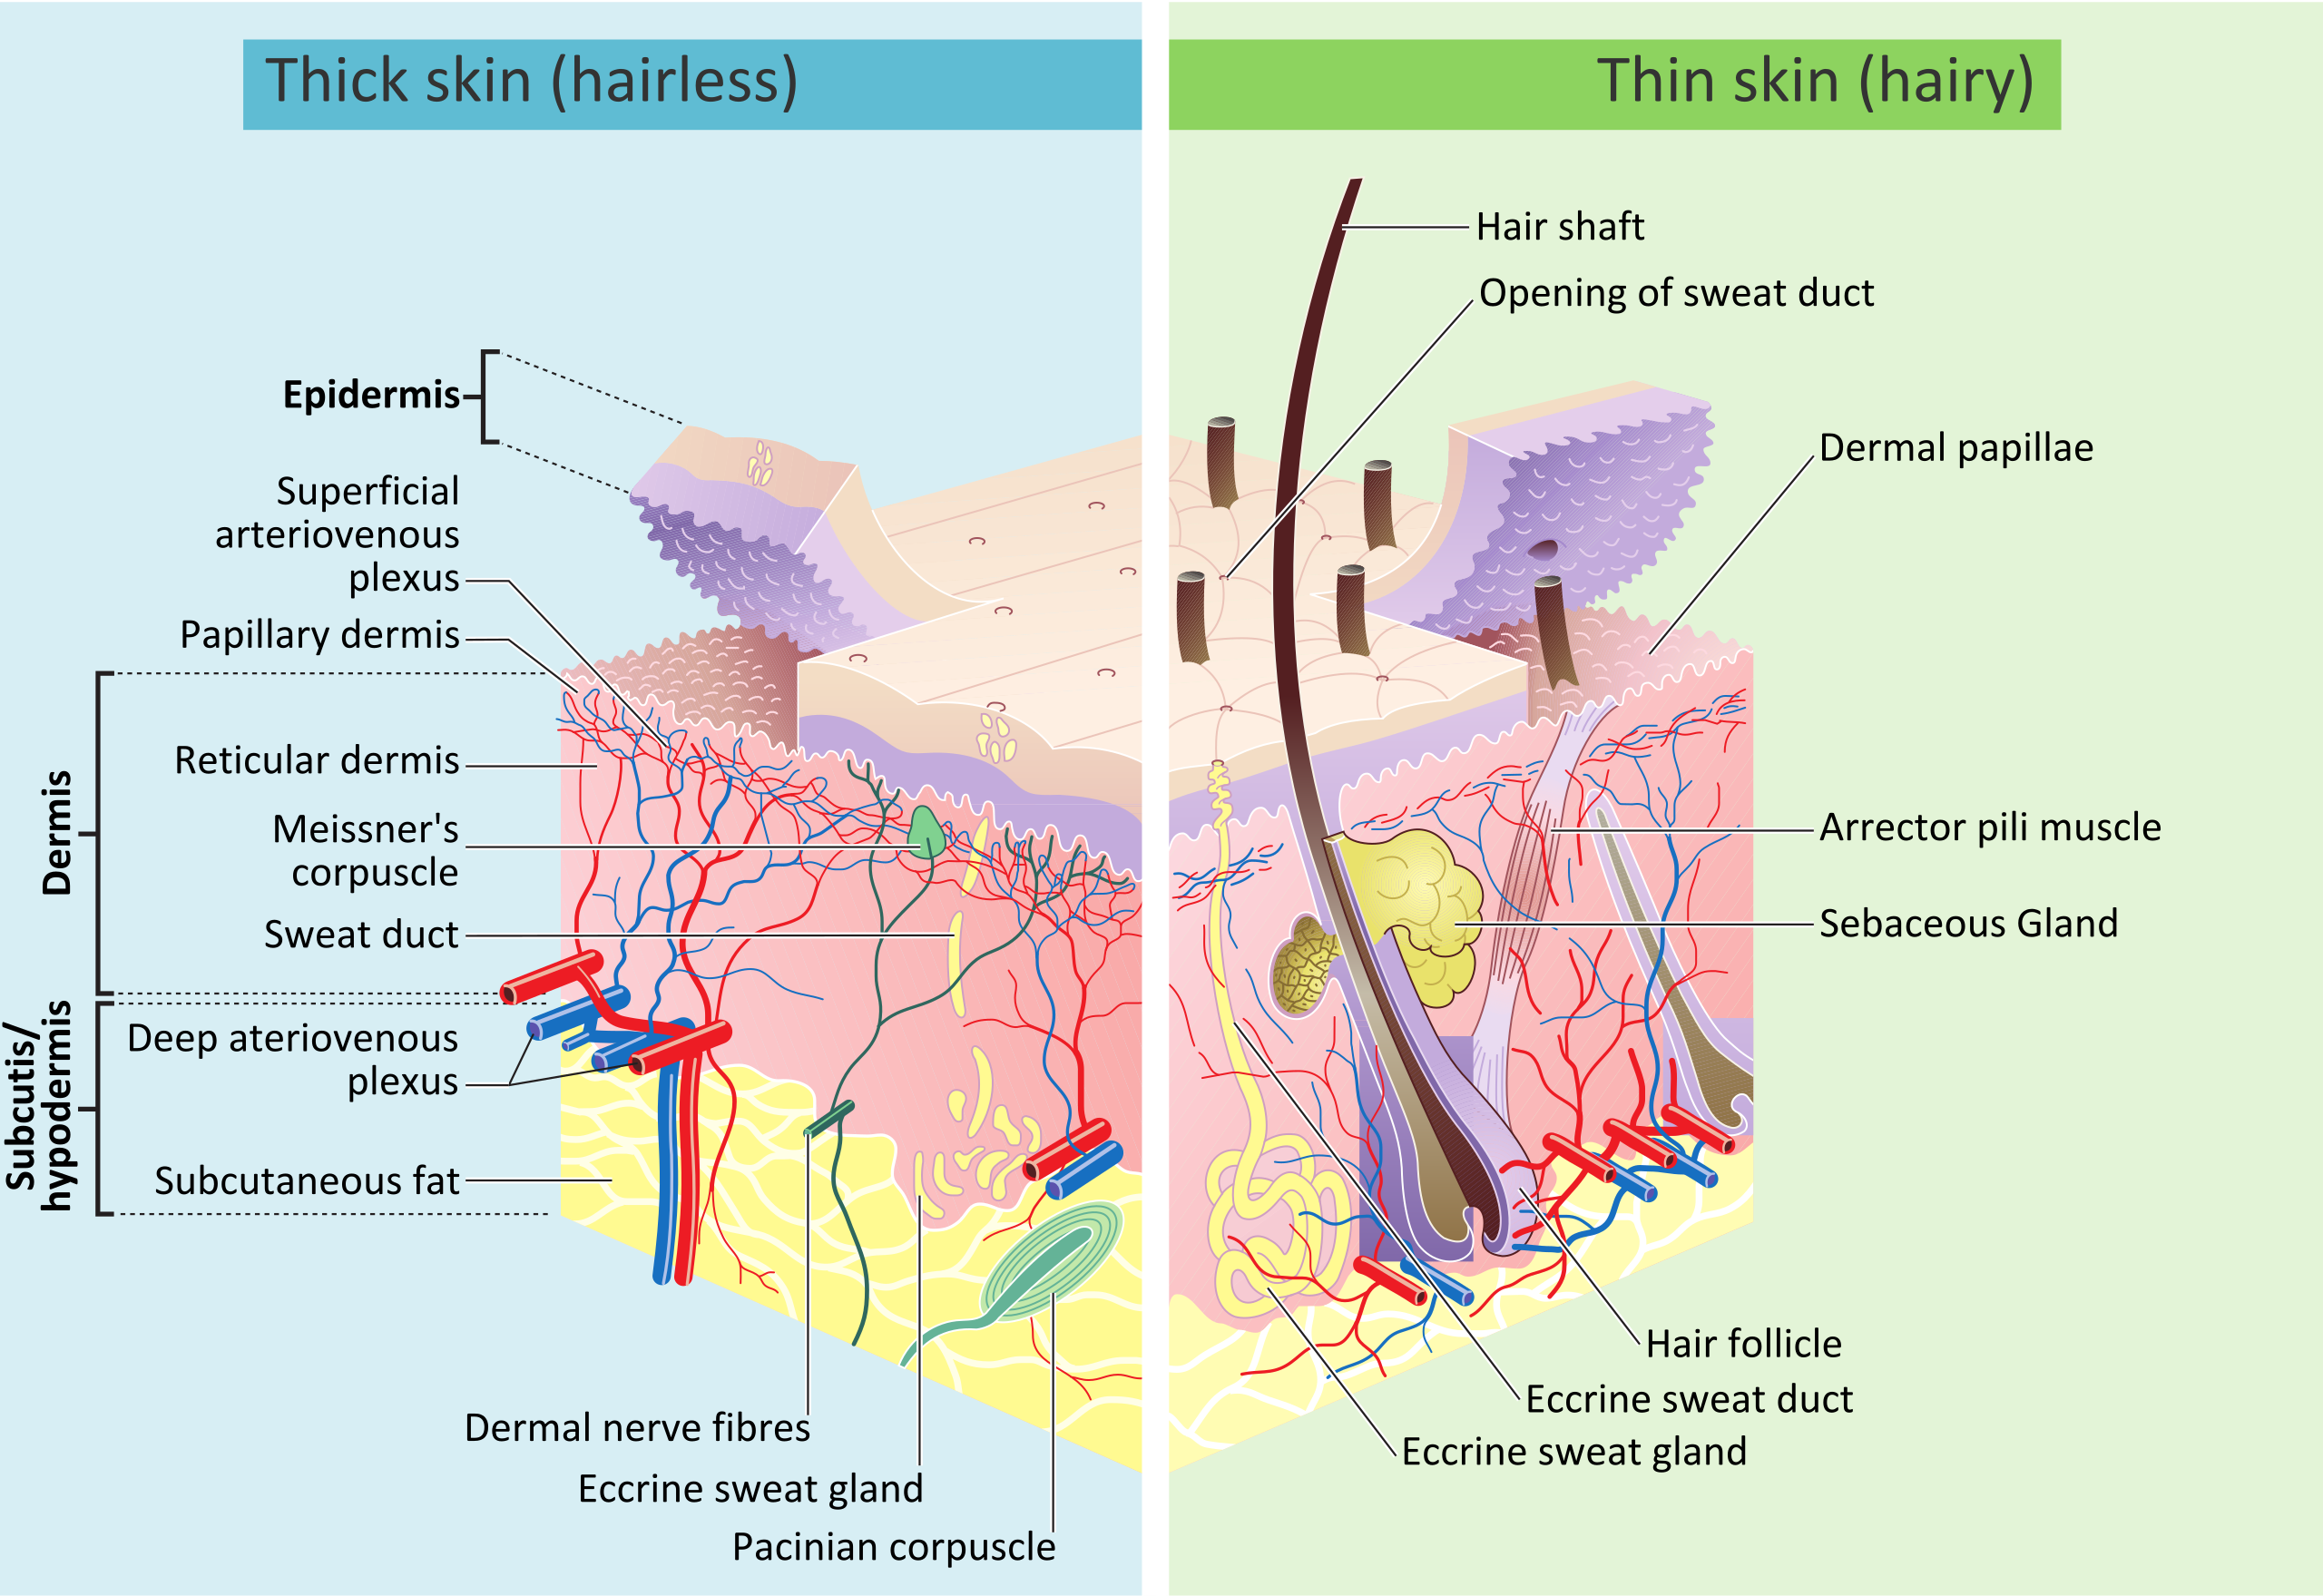
\includegraphics[width=0.85\textwidth]{kuze.png}
    \centering
    \label{}
\end{figure}

\emph{By Madhero88 and M.Komorniczak - \href{https://en.wikipedia.org/wiki/File:Skin_layers.png}{link}, CC BY-SA 3.0, \href{https://commons.wikimedia.org/w/index.php?curid=21986708}{link}}

\paragraph{Fibrocyty a fibroblasty}
\begin{myItemize}[nosep]
    \item fibrocyt je diferenciační prekurzor fibroblastu
    \item fibrocyt může diferenciovat ve fibroblast (a naopak), chondrocyt, hladkou svalovinu, tukovou buňku
    \item změna fibroblastu na tukovou buňku provázena změnou exprese genů
    \item fibroblasty vytváří desmozomy s jinými fibroblasty, vzniká síťovitá struktura
\begin{myItemize}[nosep]
    \item desmozomy jsou spojení buněk, při kterých mezi buňkami zůstávají mezery (cadheriny napojeny na intermediární filamenta)
\end{myItemize}

    \item fibroblasty spolu s epiteliálními buňkami produkují složky bazální laminy
\end{myItemize}



\paragraph{Mezenchymální kmenové buňky}
\begin{myItemize}[nosep]
    \item mají obrovský diferenciační potenciál
    \item dají se kultivovat in vitro v koktejlu růstových faktorů a cíleně diferencovat v různé typy buněk
    \item pluripotence: embryonální kmenové buňky
\begin{myItemize}[nosep]
    \item dají se izolovat z časného embrya
    \item dají se in vitro kultivovat a geneticky manipulovat a poté vrátit do embrya
\end{myItemize}

\end{myItemize}



\subsubsection{Epidermis} \label{Epidermis}


\begin{myItemize}[nosep]
    \item jediná z vrstev kůže, která je epiteliálního původu
    \item sedí na bazální lamině, nejspodnější vrstvu tvoří keratinocyty
\begin{myItemize}[nosep]
    \item v záhybech na bazální lamině jsou kmenové buňky neschopné diferencovat v melanocyty, ale vznikají z nich keratinocyty
\end{myItemize}

    \item je stále proliferována
\begin{myEnumerate}[nosep]
    \item buňky jsou posouvány vzhůru
    \item časem jsou buňky dehydratovány a keratinizují
    \item takové mrtvé buňky se odloupnou
\end{myEnumerate}

    \item obsahuje melanocyty a Langerhansovy buňky (= dendritické buňky)
    \item rozdíl mezi bělošskou a černošskou kůží je v pH endozomálního systému (běloši jsou kyselejší)
\end{myItemize}



\todo{Lépe propracovat choroby spojené s melanocyty.}

\paragraph{Melanocyty}
\begin{myItemize}[nosep]
    \item produkují melanin, kterým poté zbarvují okolní buňky
    \item ochrana před UV
    \item nevznikají v kůži, ale vlezou do ní z \hyperref[Nervové buňky]{neurální lišty}
    \item obsahují \emph{melanozomy}
\begin{myItemize}[nosep]
    \item deriváty lysozomů
    \item naplněné melaninem jsou předávány epidermálním buňkám (keratinocytům)
\end{myItemize}

    \item mutace
\begin{myItemize}[nosep]
    \item málo melanozomových prekurzorů => málo melanozomů => skvrny
    \item mutace genu pro kit
\begin{myItemize}[nosep]
    \item receptor pro SCF faktor => je na epiteliální buňce v nice => udržuje buňky                     v kmenovém stavu
    \item málo kmenových buněk => málo melanocytů
\end{myItemize}

    \item mutace v genu Pax3
\begin{myItemize}[nosep]
    \item homozygot => ztráta sluchu, depigmentace vlasů, očí, kůže
\end{myItemize}

\end{myItemize}

\end{myItemize}



Porucha tvorby melaninu vede k albinismu. Tato porucha může být způsobena poruchou v enzymu tyrozinkináze nebo poruchou regulace pH v melanozomu.

\paragraph{Langerhansovy buňky}
\begin{myItemize}[nosep]
    \item derivované z kostní dřeně
    \item dendritická buňka nesoucí MHC II
    \item tvoří jednu vrstvičku rovnoměrně rozloženou pod kůží
    \item po pohlcení cizorodých substancí čekají v uzlině na rozpoznání T-lymfocytem, který poté obstará imunitní reakci
\end{myItemize}



\subsection{Neuroepitely} \label{Neuroepitely}


\emph{Pro více informací viz \hyperref[Nervové buňky]{oddíl o nervových tkáních} a \hyperref[Senzorické epitely]{oddíl o senzorických epitelech}.}

\begin{myItemize}[nosep]
    \item mají rozdílnou schopnost regenerace a rychlost obměny buněk
\begin{myItemize}[nosep]
    \item senzorický neuroepitel ve středním uchu ani ten na sítnici není schopen regenerace (máme ho jednou pro vždy)
    \item čichový epitel prochází neustálou obměnou
\begin{myItemize}[nosep]
    \item je epidermálního původu
    \item pro detailnější popis tkáně viz \hyperref[Čichový epitel]{oddíl o čichovém epitelu}
\end{myItemize}

\end{myItemize}

\end{myItemize}



\section{Patologie} \label{Patologie} \FloatBarrier


\paragraph{Kartagenův syndrom (situs inversus)}
\begin{myItemize}[nosep]
    \item převrácená pravolevá symetrie vnitřních orgánů
    \item 50\% jedinců trpí chronickou bronchitidou a sterilitou
    \item první popsaný případ v roce 1688
    \item způsoben mutací v molekulárním motoru zajišťujícím pohyb řasinek v řasinkovém epitelu
\end{myItemize}



\paragraph{Průjem}
\begin{myItemize}[nosep]
    \item porucha funkce resorpčních epitelů trávicí soustavě
    \item u dospělého člověka je za jeden den sekrece sedmi litrů tekutin
\begin{myItemize}[nosep]
    \item 1l slin
    \item 1,5l trávicí tekutiny v žaludku
    \item 1l žluči
    \item 1,5l trávicí tekutiny ze slinivky
    \item 2l sukusu (všemožné tekutiny vylučované živými tkáněmi)
\end{myItemize}

    \item resorpce tekutin ve střevě
\begin{myItemize}[nosep]
    \item 7,8l v tenkém střevě + dvanáctníku
    \item 1l v tlustém střevě
\end{myItemize}

    \item 0,2l ztrácíme stolicí
\end{myItemize}



\paragraph{Cystická fibróza}
\begin{myItemize}[nosep]
    \item druhá nejčastější genetická porucha (po poruše konexinu vedoucí k poruše sluchu)
    \item způsobená mutací proteinu CFTR, který přenáší chloridové ionty ven z buněk
\begin{myItemize}[nosep]
    \item ve zdravé buňce dochází vylučování chloridových iontů
\begin{myItemize}[nosep]
    \item spolu s ionty opouští buňky voda
    \item dochází ke zvlhčení epitelů a sliznice
\end{myItemize}

    \item v nezdravé buňce k tomu nedochází, sliznice jsou suché, hleny jsou husté
\end{myItemize}

    \item trpí jí jeden člověk z 2500
\end{myItemize}



Existují i určité poruchy mechanických vlastnosí kůže, které jsou způsobeny hlavně mutacemi v genech pro keratiny.

\chapter{Pojivová tkáň} \label{Pojivová tkáň}


\begin{myItemize}[nosep]
    \item je tvořena různými buněčnými typy
    \item má rozmanitou strukturu, funkci i tvar
    \item produkuje velké množství ECM sekretorickou drahou (často více ECM než buněk)
    \item vazivo, chrupavky, kosti, tuková tkáň, krev
\end{myItemize}



\section{Vazivo} \label{Vazivo} \FloatBarrier


\begin{myItemize}[nosep]
    \item řídké, \emph{areorální}
\begin{myItemize}[nosep]
    \item spojuje tkáně mezi sebou
    \item obsahuje kolagenní, elastická i retikulární vlákna (obecně hodně ECM)
    \item vyplňuje prostory, zpevňuje epitely, obaluje lymfatické a krevní cévy, je ve žlázách, sliznicích, dermis
    \item typy
\begin{myItemize}[nosep]
    \item tukové
    \item elastické (okolo páteře)
    \item retikulární (vytváří prostot pro "výrobní buňky")
\end{myItemize}

\end{myItemize}

    \item husté
\begin{myItemize}[nosep]
    \item převládají kolagenní vlákna (obecně velmi málo ECM)
    \item typy
\begin{myItemize}[nosep]
    \item neuspořádané
\begin{myItemize}[nosep]
    \item svazky kolagenu bez určité orientace
    \item např. dermis (podkoží)
\end{myItemize}

    \item uspořádané
\begin{myItemize}[nosep]
    \item orientované podle stejnosměrných mechanických podnětů
    \item např. šlachy
\end{myItemize}

\end{myItemize}

\end{myItemize}

\end{myItemize}



\paragraph{Extracelulární matrix (ECM)}
\begin{myItemize}[nosep]
    \item hlavní složkou je kolagen různých typů
    \item epitel nebývá vaskularizovaný, ale pod epitelem je vaskularizovaná pojivová tkáň
\begin{myItemize}[nosep]
    \item taková tkáň obsahuje velké množství buněk imunitního systému, především bazofilů
\end{myItemize}

\end{myItemize}



\paragraph{Retikulární pojivová tkáň}
\begin{myItemize}[nosep]
    \item houbovité uspořádání s volnými prostory uvnitř
    \item vyskytuje se v místech, kde jsou třeba malé dutiny
    \item fibroblasty produkují ECM pomocí extracelulárních vláken
\begin{myItemize}[nosep]
    \item tvoří architektonickou kostru krvetvorných orgánů (kostní dřeň, uzliny, slezina) z retikulárních buněk
\end{myItemize}

\end{myItemize}



\todo{Lépe formulovat to, co dělají fibroblasty.}

\paragraph{Vaziva se speciálními vlastnostmi}
\begin{myItemize}[nosep]
    \item elastická vaziva
\begin{myItemize}[nosep]
    \item žluté vazy páteře, závěsný vaz penisu (ligamentum suspensorium penis)
\end{myItemize}

    \item rosolovité vazivo
\begin{myItemize}[nosep]
    \item amorfní hmota, tvořená kyselinou hyaluronovou
    \item rosolovitá konzistence jako výplň
    \item základní složka pupeční šňůry, v pulpách vyvíjejících se zubů
\end{myItemize}

    \item tukové vazivo
    \item hemopoetická tkáň
\begin{myItemize}[nosep]
    \item lymfatická a myeloidní tkáň
\end{myItemize}

\end{myItemize}



\section{Tuková tkáň} \label{Tuková tkáň} \FloatBarrier


\begin{myItemize}[nosep]
    \item jeden z největších orgánů v těle
\begin{myItemize}[nosep]
    \item muži: 15--20\% hmotnosti
    \item ženy: 20--25\% hmotnosti
\end{myItemize}

    \item hormonálně aktivní orgán
    \item vysoce inervovaná a vaskularizovaná
    \item po extrémním zhubnutí zůstane na ploskách nohou
    \item dělí se na žlutou a hnědou
\end{myItemize}



\paragraph{Funkce tukové tkáně}
\begin{myItemize}[nosep]
    \item tvaruje povrch těla
    \item tlumí nárazy
    \item obstarává tepelnou izolaci, slouží k produkci tepla
    \item vyplňuje prostory
    \item slouží jako zásobárna energie
\end{myItemize}



\begin{description}
\item[unilokulární tuková tkáň]\hfill \\
V každé tukové buňce je jen jedna centrálně uložená tuková kapénka.


\item[multilokulární tuková tkáň]\hfill \\
V každé tukové buňce je mnoho drobných tukových kapének.

\end{description}


\paragraph{Žlutá tuková tkáň}
\begin{myItemize}[nosep]
    \item unilokulární
    \item nemá membránu, je formována hydrofobními interakcemi
    \item barva od bílé po tmavožlutou
    \item je rozdělena vazivovými přepážkami do neúplných lalůčků
    \item vzniká diferenciací z mezenchymálních buněk
    \item rozsah: všude mimo očních víček, penisu, skrota (šourku) a ušního boltce
\begin{myItemize}[nosep]
    \item existují oblasti s aktivní inhibicí tvorby tukové tkáně
\end{myItemize}

\end{myItemize}



\paragraph{Hnědá tuková tkáň}
\begin{myItemize}[nosep]
    \item multilokulární
    \item má mnoho mitochondrií, a tedy hodně cytochromu b, z čehož plyne její hnědé zbarvení
    \item připomíná endokrinní žlázu
    \item buňky jsou inervovány sympatikem
    \item slouží k produkci tepla (netřesová termogeneze)
\begin{myEnumerate}[nosep]
    \item pokud je chladno, uvolní se norepinefrin
    \item aktivuje se senzitivní lipáza
    \item tuky jsou hydrolyzovány na triacylglyceridy
    \item protonový gradient v mitochondriích je díky UCP (uncoupling proteinu) transformován v teplo
\end{myEnumerate}

    \item novorozenec ale využije protonový gradient k výrobě ATP a teplo vyrábí třesovou termogenezí
    \item u novorozence 2-5\% hmotnosti
\end{myItemize}



\paragraph{Regulace množství tukové tkáně}
\begin{myItemize}[nosep]
    \item čím více tukové tkáně, tím více proteinu leptinu tělo produkuje
    \item leptinový receptor je v hypokampu (centrální centrum hladu a sytosti)
    \item lidé jedí více, když mají málo leptinu
\begin{myItemize}[nosep]
    \item leptin je tedy negativní regulátor velikosti tukové tkáně
\end{myItemize}

\end{myItemize}



\paragraph{Nádory tukových tkání}
\begin{myItemize}[nosep]
    \item unilokulární adipocyty
\begin{myItemize}[nosep]
    \item lipomy (benigní)
\begin{myItemize}[nosep]
    \item kuličky hypertrofované tukové tkáně
    \item díky vazivovému obalu snadné odstranění
\end{myItemize}

    \item liposarkomy (maligní)
\end{myItemize}

    \item multilokulární adipocyty
\begin{myItemize}[nosep]
    \item hibernomy (benigní)
\begin{myItemize}[nosep]
    \item hypertrofovaná multilokulární tuková tkáň
    \item poruchy produkce tepla
\end{myItemize}

\end{myItemize}

\end{myItemize}



\section{Chrupavka} \label{Chrupavka} \FloatBarrier


\begin{myItemize}[nosep]
    \item mezibuněčná hmota nabývá pevné konzistence
    \item není inervovaná ani vaskularizovaná
\begin{myItemize}[nosep]
    \item nemůže bolet
    \item je živena difúzí z přilehlé vazivové tkáně (perichondria)
\end{myItemize}

    \item růst chrupavky
\begin{myItemize}[nosep]
    \item buňky jsou zalité v ECM, to jim umožňuje růst a dělení (v omezené míře)
\begin{myItemize}[nosep]
    \item čtyři buněčná dělení maximálně osmi buněk v lakunách (malých kanálcích)
\end{myItemize}

\end{myItemize}

\end{myItemize}



\todo{Jakým způsobem je omezeno dělení?}

\paragraph{Funkce}
\begin{myItemize}[nosep]
    \item podpora měkkých tkání
    \item tlumí nárazy
    \item umožňuje hladký klouzavý pohyb kostí
    \item zásadní pro vývoj kostí
\end{myItemize}



\paragraph{Složení}
\begin{myItemize}[nosep]
    \item ECM (tedy hlavně kolagenní vlákna)
    \item proteoglykany orientované na kolagenních a elastických vláknech
    \item glykosaminoglykany
    \item chondrocyty
\end{myItemize}



\paragraph{Chondroblasty}
\begin{myItemize}[nosep]
    \item vznikají diferenciací mezenchymálních kmenových buněk na povrchu chrupavky
\begin{myItemize}[nosep]
    \item těmto buňkám se někdy také říká osteprogenitoriální buňky
\end{myItemize}

    \item jedny z mála buněk schopné přežít v jedinci i po smrti
    \item fungují díky anaerobní glykolýze
    \item jejich proliferace je ovlivňována růstovými faktory
\begin{myItemize}[nosep]
    \item \emph{somatotropin} spouští produkci somatomedinu v játrech
    \item nedostatek způsobuje metaplázii chrupavek
\end{myItemize}

    \item tvoří a obalují se ECM, tím se dostávají dovnitř do chrupavky
\end{myItemize}



\paragraph{Chondrocyty}
\begin{myItemize}[nosep]
    \item buněčná složka chrupavky
    \item většinou už ECM neprodukují, ale někdy ano
    \item nalézají se \emph{v lakunách} v tzv. isogenetických skupinkách (skupinkách chondrocytů, které všechny vznikly z jediné osteprogenitoriální buňky)
    \item odolávají nízkému parciálnímu tlaku kyslíku
\begin{myItemize}[nosep]
    \item jsou často vystaveny nedostatku kyslíku
\end{myItemize}

\end{myItemize}



\todo{Zjistit, co je EK.}

\paragraph{Typy chrupavek}
\begin{myItemize}[nosep]
    \item hyalinní
\begin{myItemize}[nosep]
    \item nejběžnější
    \item kolagen (40\% suché váhy, hlavně typu II), chondroitin-6-sulfát, keratan sulfát, chondronektin
    \item modravě bílá a průsvitná
    \item v zárodku vytváří dočasný skeleton, který je nahrazen kostní tkání
    \item např. artikulační plochy pohyblivých kloubů, nos, hrtan, trachea, bronchy, přední konce žeber
\end{myItemize}

    \item elastická
\begin{myItemize}[nosep]
    \item ohebná, roztažitelná
    \item nažloutlá barva
    \item velké množství elastinových vláken, kolagen
    \item např. ušní boltec, stěny zevního zvukovodu, Eustachova trubice, drobné chrupavky hrtanu
\end{myItemize}

    \item vazivová
\begin{myItemize}[nosep]
    \item kolagen typu I
    \item je především v místech s velkými nároky na mechanickou odolnost a zátěž
    \item např. přechod mezi hustým vazivem a hyalinní chrupavkou: meziobratlové ploténky, spona pánevní, úpony některých vazů
\begin{myItemize}[nosep]
    \item výhřez meziobratlové ploténky (ruptura anulus fibrosu)
\begin{myEnumerate}[nosep]
    \item vypuzení tekutého pulpózního jádra
    \item oploštění celého fibrózního prstence
    \item dislokace
\end{myEnumerate}

\end{myItemize}

\end{myItemize}

\end{myItemize}



\paragraph{Patologie}
\begin{myItemize}[nosep]
    \item benigní nádory (chondromy)
    \item maligní nádory (chondrosarkomy)
    \item kalcifikace (zvápenatění)
    \item záněty perichondria
    \item špatná regenerace v dospělém věku
    \item achondroplázie
\begin{myItemize}[nosep]
    \item z 99\% je příčina v mutaci genu pro FGF-receptor-3
    \item ovlivňuje vývoj chrupavek v dlouhých kostech
\end{myItemize}

\end{myItemize}



\section{Kost} \label{Kost} \FloatBarrier


\begin{myItemize}[nosep]
    \item nejodolnější vůči mechanickým silám
    \item tvoří hlavní část skeletu dospělce
    \item je to specializovaná pojivová tkáň tvořená zvápenatělou mezibuněčnou hmotou
\begin{myItemize}[nosep]
    \item kostní matrix \(+\) buňky (osteoblasty, osteocyty, osteoklasty)
    \item odvápněná kost má tvar a ohebnost srovnatelnou se šlachou
\end{myItemize}

\end{myItemize}




\paragraph{Funkce}
\begin{myItemize}[nosep]
    \item dělá oporu měkkým tkáním
    \item chrání krvetvorné orgány, mozek, míchu
    \item slouží jako zásobárna vápníku a fosfátu
\end{myItemize}



\begin{figure}
    \caption{Schematický obrázek kosti}
    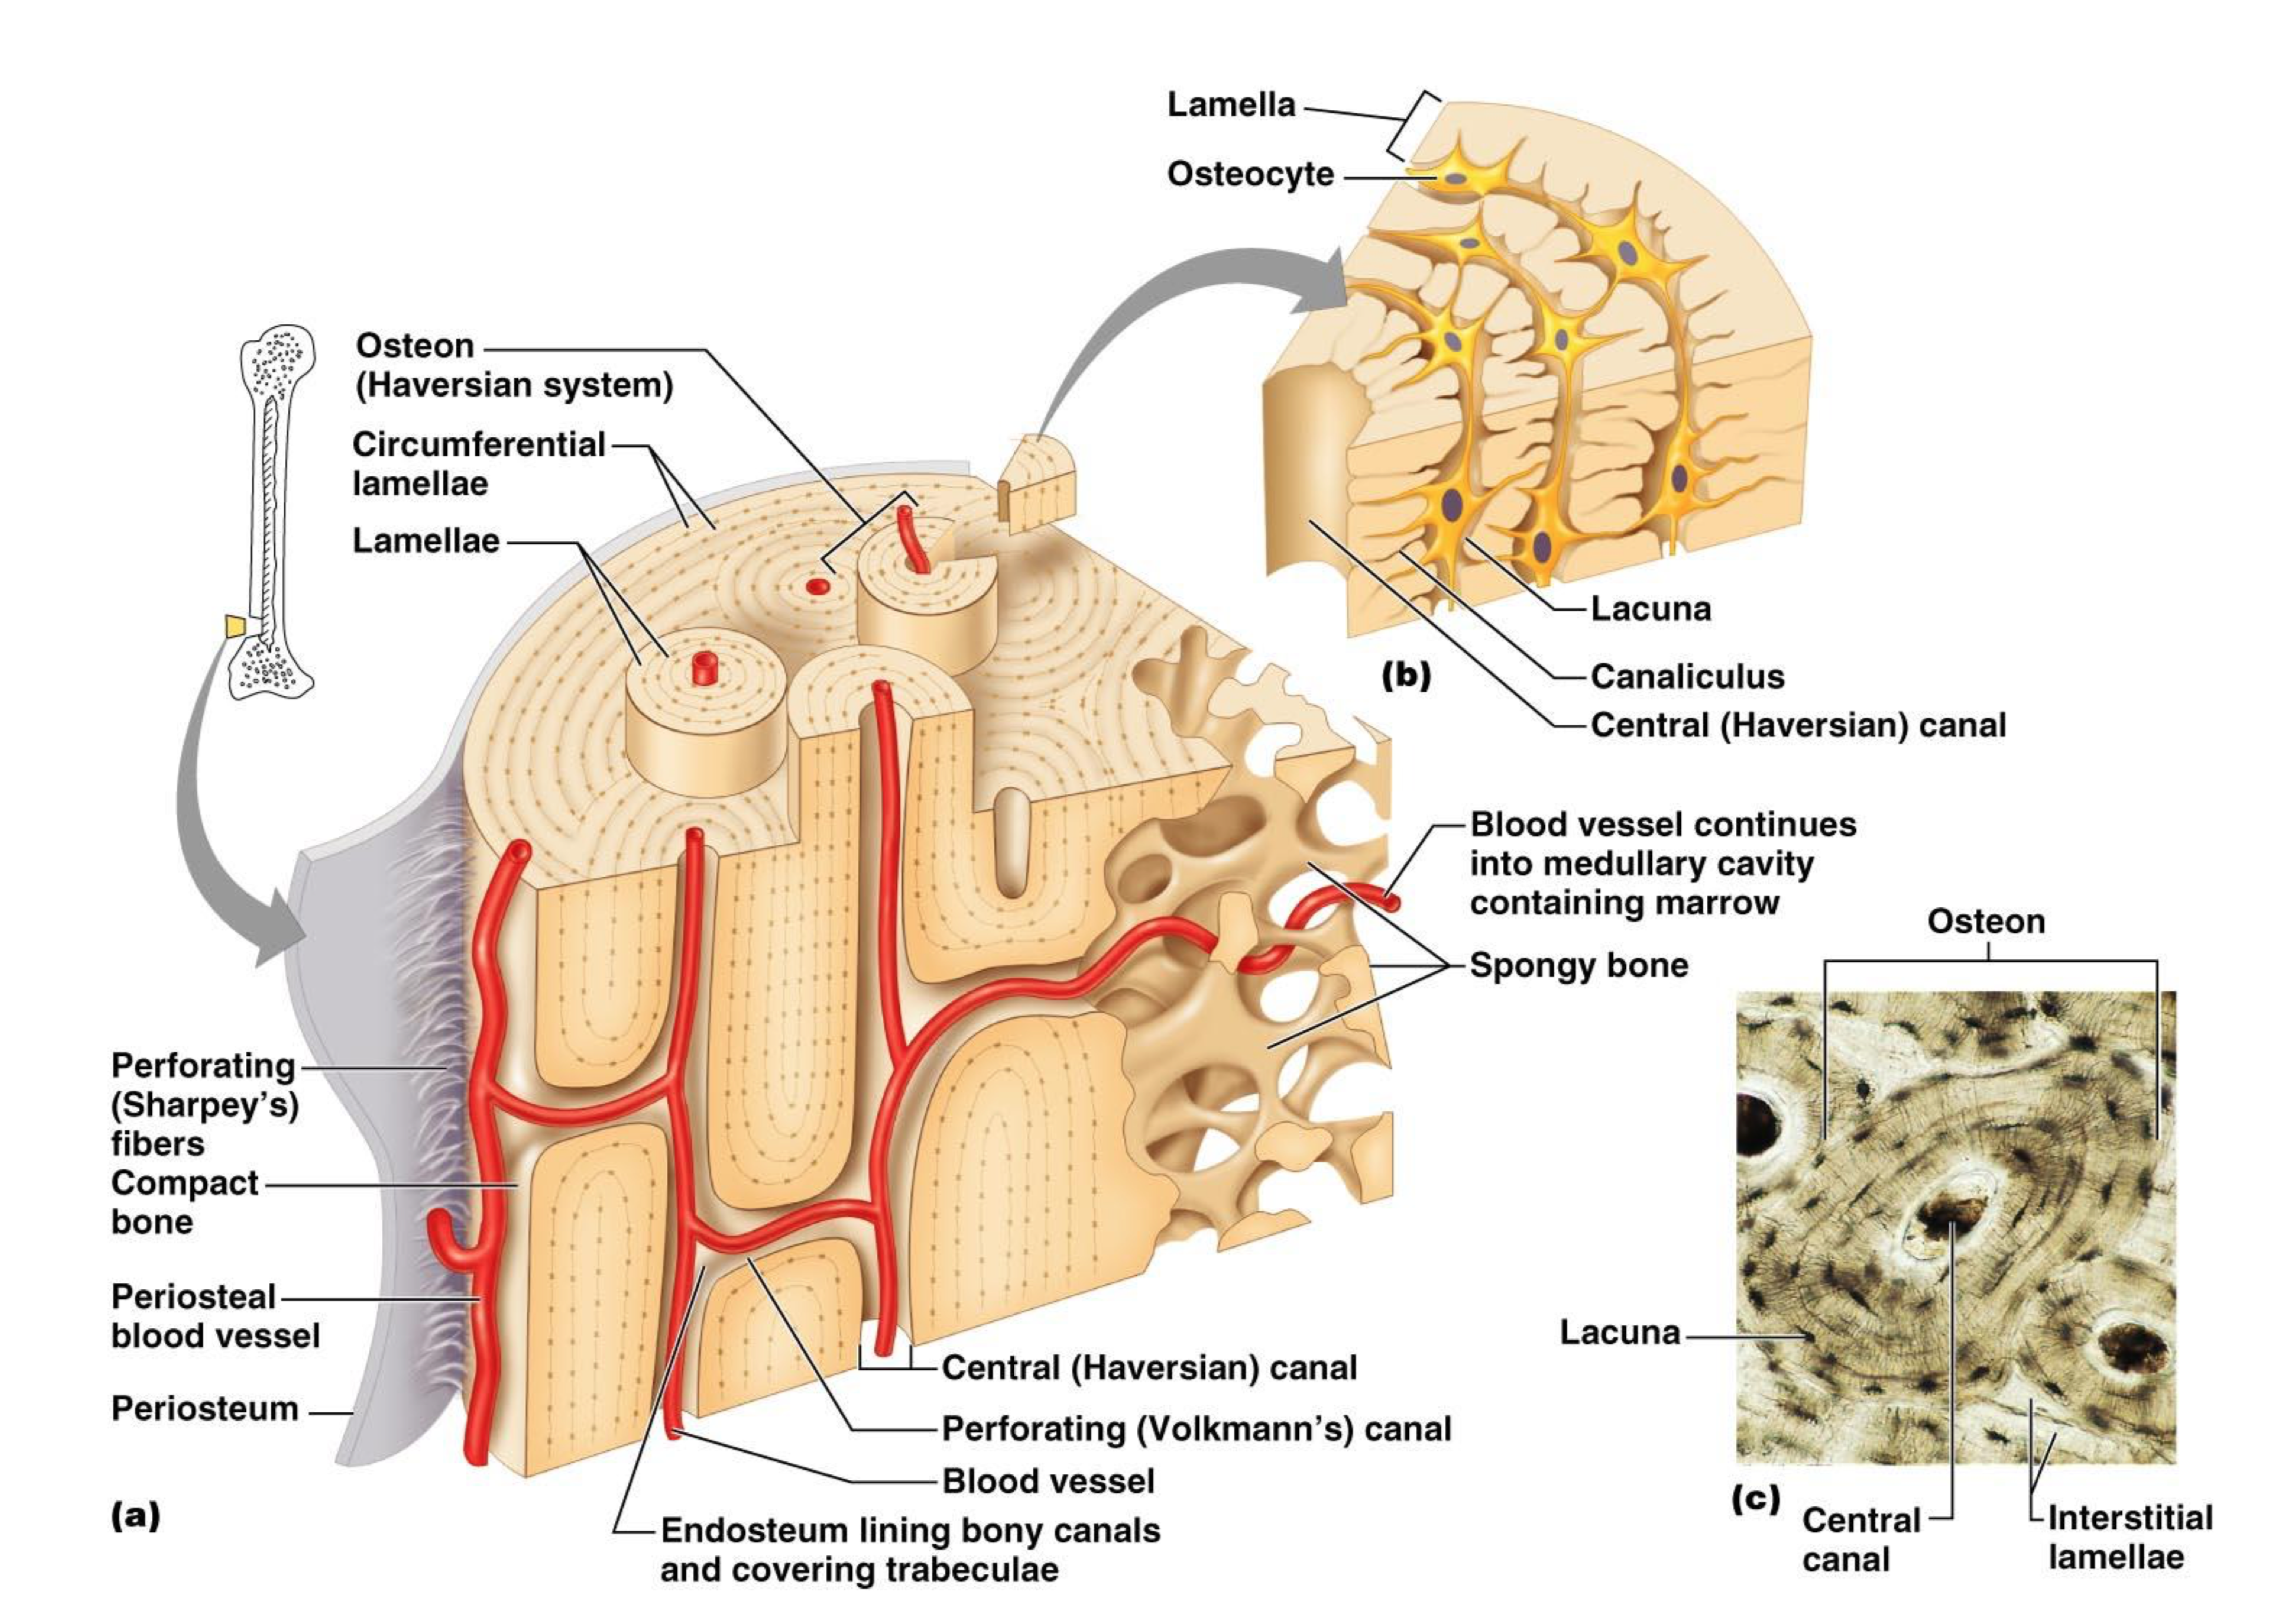
\includegraphics[width=0.85\textwidth]{kost.png}
    \centering
    \label{}
\end{figure}


\paragraph{Stavba a složení}
\begin{myItemize}[nosep]
    \item látkové složení
\begin{myItemize}[nosep]
    \item 70\% anorganické složky
\begin{myItemize}[nosep]
    \item krystaly solí, hydroxyapatit
\end{myItemize}

    \item 20\% organické složky
\begin{myItemize}[nosep]
    \item 90\% kolagen, z něj 90\% kolagen I
\end{myItemize}

    \item 10\% voda
\end{myItemize}

    \item klíčové kostní proteiny: sialoprotein, osteokalcin, osteonektin
    \item topologické složení
\begin{myItemize}[nosep]
    \item kost je síťovina osteocytů pospojovaných výběžky, které jsou propojeny přes gap junctions
    \item tato síťovina je koncentricky uspořádána do lamel kolem centrálního Haversova kanálku s cévami a nervy
    \item Haversovy kanálky jsou propojeny příčnými Volkmanovými kanálky, které přivádí cévy
    \item osteon roste dovnitř
    \item Haversovy kanálky jsou rovnoběžné s hlavní osou diafýzy
\end{myItemize}

    \item periost je vrstva na povrchu kosti
\begin{myItemize}[nosep]
    \item složen z kolagenních vláken a fibroblastů
    \item tvoří vnitřní vrstvu osteoprogenitorové buňky
    \item účel: výživa kostní tkáně, kontinuální přísun nových osteoblastů
\end{myItemize}

    \item endost vystýlá vnitřní povrch kostních dutin
\begin{myItemize}[nosep]
    \item je v něm uložena vrstva osteoprogenitorových buněk
    \item účel: výživa kostní tkáně, kontinuální přísun nových osteoblastů
\end{myItemize}

\end{myItemize}



\paragraph{Typy kostní tkáně}
\begin{myItemize}[nosep]
    \item primární nezralá vláknitá kost, sekundární zralá lamelózní kost
    \item kompaktní kost (diafýza), spongiózní kost (epifýza)
    \item krátké kosti jsou tvořeny spongiózním jádrem obklopeným kompaktní diafýzou
\begin{myItemize}[nosep]
    \item dutiny spongiózní kosti tvoří kostní dřeň
\begin{myItemize}[nosep]
    \item červená je krvetvorná
    \item žlutá obsahuje tukové buňky
\end{myItemize}

\end{myItemize}

    \item ploché kosti lebeční klenby jsou tvořeny dvěma lamelárními kompakty oddělenými vrstvou spongiózní kosti (diploe)
\end{myItemize}




\paragraph{Remodelace kostí}
\begin{myItemize}[nosep]
    \item kost se neustále přestavuje
    \item u dětí je remodelace 200\(\times\) rychlejší než u dospělých
    \item za týden se odbourá 5--7\% kostní hmoty
    \item houbovitá část je obnovována jednou za 3--4 roky
    \item kompaktní část je obnovována jednou za 10 let
    \item resorpce je regulována osteoklasty
\end{myItemize}



\subsection{Kostní buňky} \label{Kostní buňky}


\paragraph{Osteoblasty}
\begin{myItemize}[nosep]
    \item vznik z mezenchymálních kmenových buněk
    \item po uhnízdění se mění v osteocyty
    \item vytvářejí organickou ECM
\begin{myItemize}[nosep]
    \item provádí syntézu kolagenu I, proteoglykanů, glykoproteinů
\end{myItemize}

    \item jsou lokalizovány výhradně na povrchu kosti, těsně vedle sebe jako jednovrstevný epitel
    \item kontakt s ostatními buňkami skrz výběžky
\end{myItemize}



Výstavbovou aktivitu kostní matrix můžeme měřit tetracyklinem, který se váže do kostní matrix, u níž je právě v průběhu mineralizace. Druhá dávka tetracyklinu se podá tři týdny po první a měří se rozdíl mezi pozorováními.

\paragraph{Osteocyty}
\begin{myItemize}[nosep]
    \item vznikají z osteoblastů, poté co jsou uzavřeny v kosterní hmotě
    \item zaniknou, když převáží resorpce matrix
    \item spočívají v lakunách mezi lamelami matrix
    \item jejich výběžky jsou mezi buňkami propojeny gap junctions
    \item mají tvar broušeného diamantu
    \item jsou odpovědné za mineralizaci kostí
\end{myItemize}



\paragraph{Osteoklasty}
\begin{myItemize}[nosep]
    \item vznikají fúzí monocytů nebo makrofágů
    \item obrovské mnohojaderné buňky (i přes \si{100 \mu m}) s 5--50 jádry
    \item jsou bohatě větvené, pohyblivé
    \item resorbují kostní hmotu
    \item podílejí se na přestavbě kosti
    \item extracelulárně snižují pH a naleptávají kostní osteon (Haversův systém)
\begin{myItemize}[nosep]
    \item v místě resorpce vznikají enzymaticky vyleptané prolákliny v matrix, tzv. \emph{Howshipovy lakuny}
\end{myItemize}

\end{myItemize}



\subsection{Osifikace} \label{Osifikace}


\todo{Propracovat osifikaci více do detailu, opravit vývoj kostních buněk.}

\paragraph{Osifikace}
\begin{myItemize}[nosep]
    \item vývoj kostních buněk: mezenchymální buňka -> chondroblast -> chondrocyt
    \item dělení
\begin{myItemize}[nosep]
    \item intramembranózní
\begin{myItemize}[nosep]
    \item probíhá ve vazivu, kost vzniká přeměnou vaziva
\begin{myItemize}[nosep]
    \item probíhá přímá mineralizace matrix produkované osteoblasty
\end{myItemize}

    \item růst plochých a krátkých kostí, zvětšování dlouhých kostí do šířky, formování lebky, hojení zlomenin
\end{myItemize}

    \item endochondrální osifikace
\begin{myItemize}[nosep]
    \item kost vzniká náhradou chrupavky
\begin{myItemize}[nosep]
    \item probíhá ukládání kostní matrix a anorganických složek na předem vytvořenou matrix chrupavky
\end{myItemize}

    \item vznik dlouhých a krátkých kosti
 - vhodné prostředí zajišťují mezenchymální buňky a fibroblasty
\end{myItemize}

\end{myItemize}

    \item kost může po splnění určitých podmínek vzniknout kdekoli v těle
    \item chrupavka může také osifikovat (speciální případ metaplazie)
\begin{myEnumerate}[nosep]
    \item v chrupavce je zánět
    \item je vyslán signál nebezpečí k cévám
    \item cévy vysílají výběžky do chrupavky, směrem k zánětu, aby jej odstranily
    \item chrupavka je transformována v kost
\end{myEnumerate}

\end{myItemize}



\paragraph{Průběh intramembranózní osifikace}
\begin{myEnumerate}[nosep]
    \item nahromadění mezenchymálních kmenových buněk (MSC)
    \item vznik nidu, skupiny MSC
    \item diferenciace MSC v osteoblasty
    \item osteoblasty tvoří kostní matrix (vylučují mimo jiné osteoidy)
    \item kostní matrix je mineralizována
    \item radiální růst nidů vedoucí k jejich splynutí
\end{myEnumerate}



\paragraph{Průběh endochondrální osifikace}
\begin{myEnumerate}[nosep]
    \item vznikne periosteum, ze kterého se časem začnou uvolňovat osteoblasty
    \item osteoblasty začnou uvolňovat osteoid, který se ukládá kolem existující chrupavky
    \item chondrocyty se zvětší, žačnou produkovat alkalin fosfatázu, která přispěje k mineralizaci kostní matrix
    \item osteoprogenitorové buňky začnou na matrix ukládat další osteoid
\end{myEnumerate}



Počet osteoklastů zvyšuje parathormon. Při velkém množství parathormonu tedy dochází k odbourávání kosti, k osteoporóze a k následnému uvolnění \(\ce{Ca^{2+}}\) do krve. Naopak kalcitonin resorpci matrix inhibuje.

\subsection{Patologie} \label{Patologie}


\paragraph{Zlomeniny}
\begin{myItemize}[nosep]
    \item kost praskne
    \item existují mutace ovlivňující poměr odbourávání a budování kostní hmoty
\begin{myItemize}[nosep]
    \item důsledkem je např. osteopetróza, osteoporóza
\end{myItemize}

    \item průběh zloměniny
\begin{myEnumerate}[nosep]
    \item po zlomení se aktivují osteoblasty, namnoží se
    \item osteblasty vytvoří houbovitou kost
    \item houbovitá kost je postupně přestavena v kompaktní kost
\end{myEnumerate}

    \item krátké kosti se hojí špatně, zatímco dlouhé jsou na mechanické změny zvyklé
\end{myItemize}



\paragraph{Poruchy kostní tkáně}
\begin{myItemize}[nosep]
    \item rachitis
\begin{myItemize}[nosep]
    \item nedostatek vápníku u dětí, je narušen osifikační proces
\end{myItemize}

    \item osteomalacie
\begin{myItemize}[nosep]
    \item nedostatek vápníku u dospělých (těhotenství), měknutí kostí
\end{myItemize}

    \item osteoporóza
\begin{myItemize}[nosep]
    \item rozpad kostní hmoty (přílišná aktivita osteoklastů)
    \item opakem je osteopetróza
\end{myItemize}

    \item gigantismus
\begin{myItemize}[nosep]
    \item přílišný růst kostí, člověk je nadprůměrně veliký
    \item příčinou je přebytek růstového hormonu
    \item opakem je hypofyzární nanismus
\end{myItemize}

    \item akromegalie
\begin{myItemize}[nosep]
    \item většinou zvětšení čela, nosu, lícních kostí, spojená s bolestí kloubů
    \item příčinou je nadbytek růstového hormonu v dospělosti
\end{myItemize}

    \item Pagetova choroba
\begin{myItemize}[nosep]
    \item kosti jsou deformované
    \item příčinou je přílišné odbourávání kostí spojené s rychlým a neorganizovaným růstem nové kostní tkáně
\begin{myItemize}[nosep]
    \item problém v metabolismu a diferenciaci osteoklastů
\end{myItemize}

    \item je léčitelná transplantací kostní dřeně
\end{myItemize}

\end{myItemize}



\section{Krev} \label{Krev} \FloatBarrier


\meta{Tato kapitola bývá probírána až v rámci posledních přednášek, po nervové soustavě.}


\paragraph{Linie krevních buněk}
\begin{myItemize}[nosep]
    \item erytroidní linie
\begin{myItemize}[nosep]
    \item zprostředkování transportu kyslíku do tkání
    \item erytrocyty, retikulocyty
\end{myItemize}

    \item lymfoidní linie
\begin{myItemize}[nosep]
    \item zásadní pro tvorbu adaptivní imunitní odpovědi
    \item T-buňky, B-buňky a jejich blízcí příbuzní
\end{myItemize}

    \item myeloidní linie
\begin{myItemize}[nosep]
    \item umožňuje vrozenou imunitní odpověď a podílí se na odpovědi adaptivní
    \item granulocyty a makrofágy
\end{myItemize}

\end{myItemize}



\begin{figure}
    \caption{Schéma zobrazující vývoj krevních buněk ze společné kmenové buňky}
    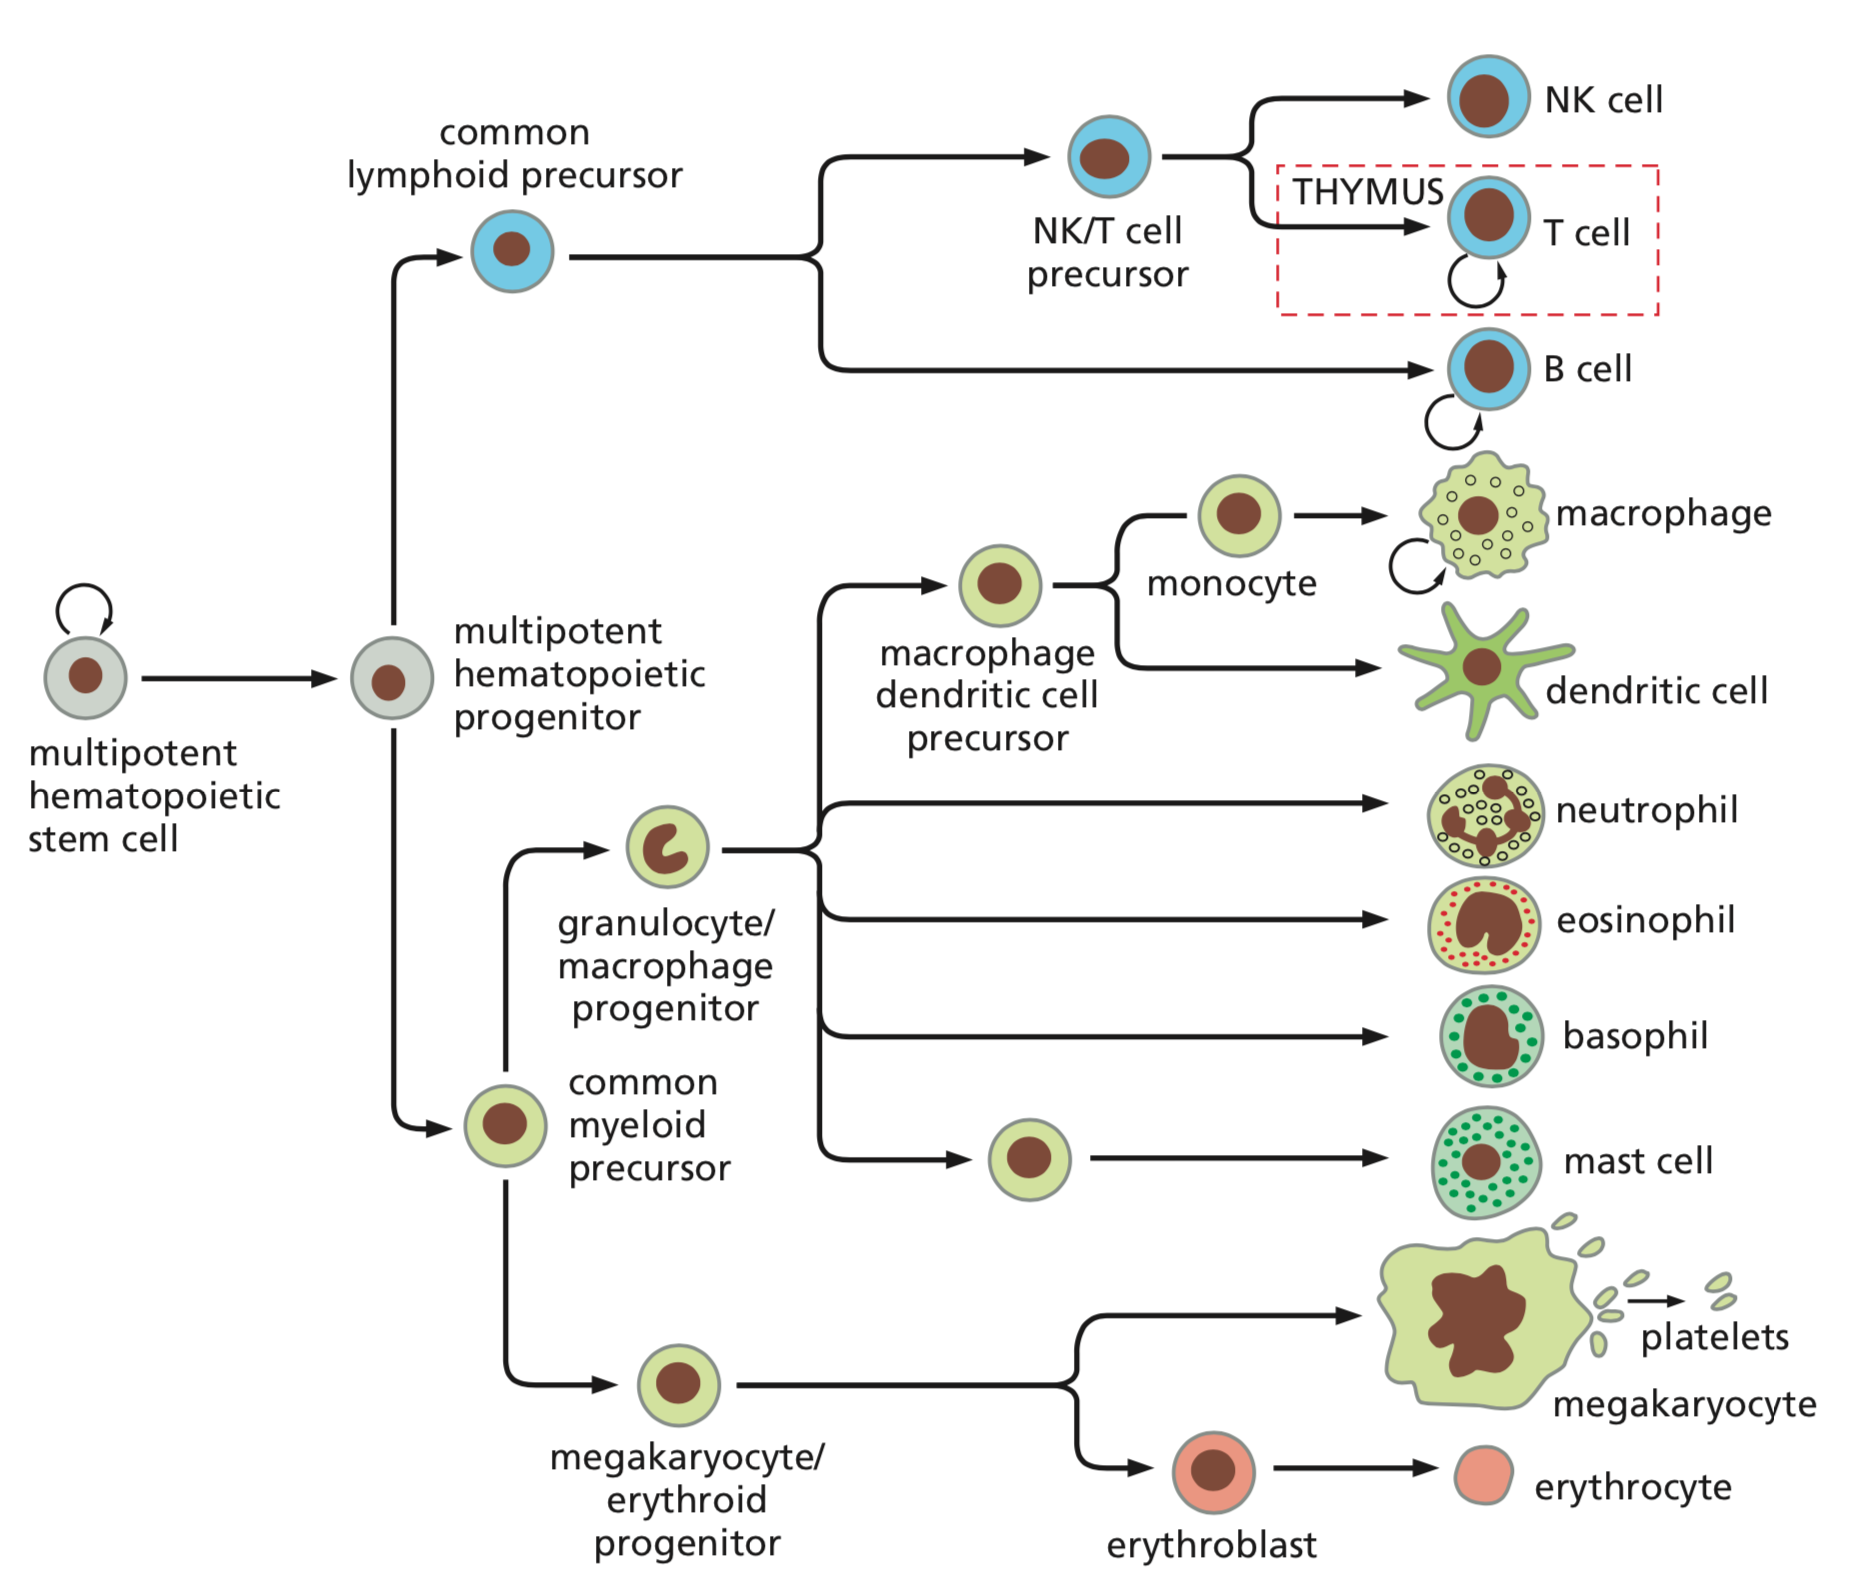
\includegraphics[width=0.85\textwidth]{vyvoj_krevinch_bunek.png}
    \centering
    \label{}
\end{figure}


\begin{description}
\item[hematokrit]\hfill \\
Celkový objem pevné složky krve.

\end{description}


\paragraph{Složení krve}
\begin{myItemize}[nosep]
    \item objev krve činí 6 až 8\% tělesné hmotnosti
\begin{myItemize}[nosep]
    \item z toho hematokrit činí u žen 41\%, u mužů 46\%
\end{myItemize}

    \item hodně mezibuněčné hmoty (plazma)
\begin{myItemize}[nosep]
    \item nestlačitelná
    \item 5--6 litrů
\end{myItemize}

    \item krevní buňky: erytrocyty, leukocyty, trombocyty
\begin{myItemize}[nosep]
    \item relativně mobilní, schopny opustit krevní řečiště
\end{myItemize}

    \item červené krvinky (erytrocyty)
\begin{myItemize}[nosep]
    \item 45\% objemu (\si{5e12} na litr)
\end{myItemize}

    \item bílé krvinky (leukocyty)
\begin{myItemize}[nosep]
    \item 1\% objemu (\si{4} až \si{6e9} na litr)
    \item granulocyty (\si{5e9} na litr)
    \item agranulocyty (\si{7e8} na litr)
\end{myItemize}

    \item krevní destičky (trombocyty)
\begin{myItemize}[nosep]
    \item \si{150} až \si{300e9} na litr
\end{myItemize}

\end{myItemize}



\paragraph{Sedimentace}
\begin{myItemize}[nosep]
    \item její rychlost určována diagnostickou hematologickou metodou
    \item krev se nasaje do trubice, nechá se sedimentovat
\begin{myItemize}[nosep]
    \item nejrychleji klesají erytrocyty, pak leukocyty
    \item nad nimi zůstane plazma
\end{myItemize}

    \item vysoká sedimentace
\begin{myItemize}[nosep]
    \item když je v těle zánět, v plazmě je hodně imunoglobulinů
\begin{myItemize}[nosep]
    \item krev je hustější a krvinky klesají pomaleji
    \item sloupec erytrocytů je vyšší, i když jich je stejně jako u zdravého jedince
\end{myItemize}

\end{myItemize}

\end{myItemize}



\begin{description}
\item[buffy coat]\hfill \\
Koncentrovaná suspenze leukocytů a trombocytů získaná sedimentací.

\end{description}


Rychlejší alternativou sedimentace je centrifugace. K dalším metodám zkoumání krve patří krevní roztěr a průtoková cytometrie (schéma funkce viz obrázek níže).

\begin{figure}
    \caption{Schéma průtokové cytometrie}
    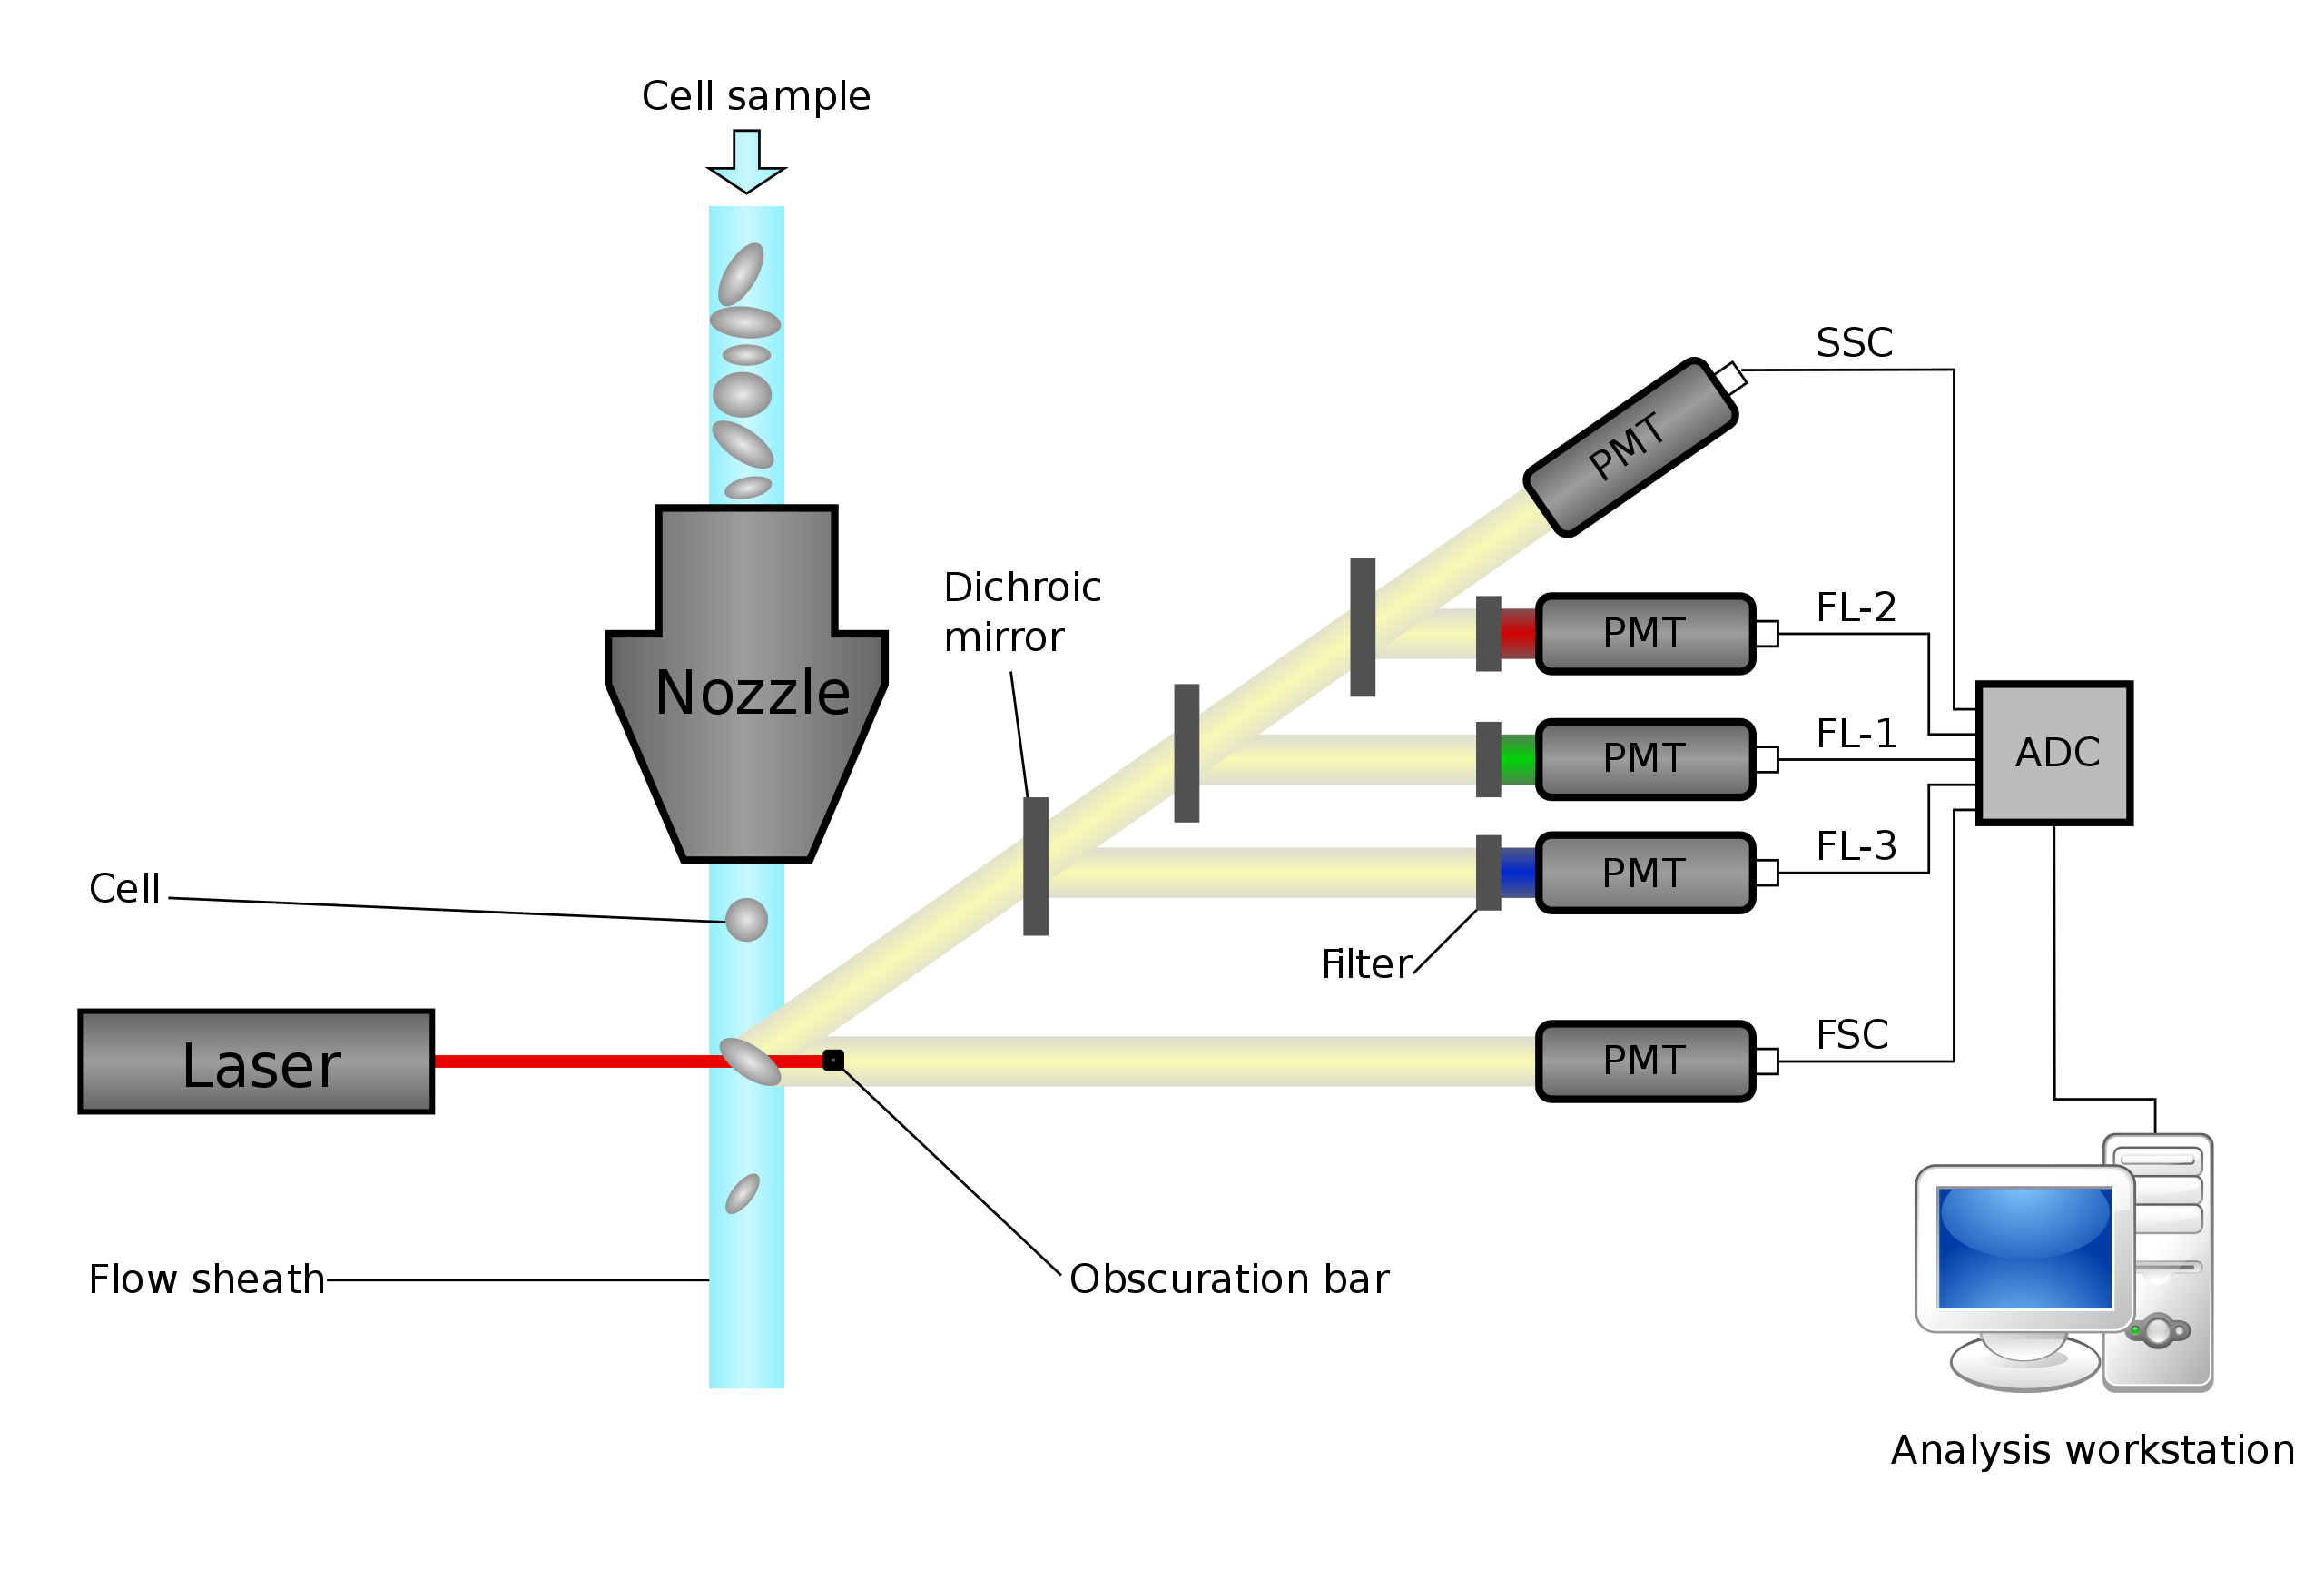
\includegraphics[width=0.85\textwidth]{cytometrie.png}
    \centering
    \label{}
\end{figure}

\emph{By Kierano - Own work, CC BY 3.0, \href{https://commons.wikimedia.org/w/index.php?curid=22102570}{link}}

Při cytometrii protékají měřičem buňky jedna po jedné. Přerušují u toho laserový paprsek, který je poté pomocí soustavy zrcadel a detektorů analyzován --- dá se zjistit počet buněk, z vlastností paprsku pak i jejich druh a obsah. Často se buňky fluorescenčně barví.

\subsection{Erytrocyty} \label{Erytrocyty}


\begin{myItemize}[nosep]
    \item terminálně diferencované bezjaderné buňky
    \item zajišťují přenos plynů (u savců)
    \item bikonkávní tvar (maximální povrch vůči objemu)
\begin{myItemize}[nosep]
    \item ptáci a obojživelníci mají oválný
\end{myItemize}

    \item průměr \si{5 \mu m}
\begin{myItemize}[nosep]
    \item kapiláry mají jen tak velký průměr, jak velké je jádro erytrocytů, které limituje jejich velikost
\end{myItemize}

    \item žijí cca 120 dní, poté jsou ve slezině či kostní dřeni odstaněny makrofágy
    \item fetální hemoglobin má vyšší afinitu ke kysíku než dospělý
\begin{myItemize}[nosep]
    \item váže kyslík za nižšího tlaku (který je v placentě)
\end{myItemize}

\end{myItemize}



\begin{description}
\item[erytroblast]\hfill \\
Nezralý erytrocyt v kostní dřeni.


\item[retikulocyt]\hfill \\
Nezralý erytrocyt v krevním řečišti (tvoří 1\% všech erytrocytů). Tyto erytrocyty neopouštějí krevní řečiště.

\end{description}


\paragraph{Vznik}
\begin{myItemize}[nosep]
    \item jako všechna pojiva pochází z mezenchymálních kmenových buněk
    \item odvozeny od kmenových buněk krevní řady (erytroidní linie)
\begin{myItemize}[nosep]
    \item ty mají extraembryonální původ (v prenatálním vývoji), vznikají ve žloutkovém váčku (trofoblastu)
\end{myItemize}

    \item vznik v kostní dřeni (\si{5e11} za den vzniká a zaniká)
    \item při změně erytroblastu v erytrocyt ztrácí erytroblast RNA, jeho jádro kondenzuje, je vyloučeno a odklizeno makrofágy (ztrácí všechny organely)
\end{myItemize}



\paragraph{Anémie (chudokrevnost)}
\begin{myItemize}[nosep]
    \item hypochromní anémie
\begin{myItemize}[nosep]
    \item erytrocytů je v krvi dost, je v nich ale nedostatek hemoglobinu
    \item v důsledku toho špatně nesou kyslík
\end{myItemize}

    \item srpkovitá anémie
\begin{myItemize}[nosep]
    \item způsobena bodovou mutací hydrofilní kyseliny glutamové (např. kodon GAA) na hydrofobní valin (např. kodon GUA)
    \item v neokysličeném stavu se hemoglobin shlukuje (polymerizuje, vytváří vláknité útvary a agregáty) a mění tak tvar krvinek
    \item krvinky mají kratší životnost, jsou méně flexibilní - blokují vlásečnice, což vede k ucpání cév
\end{myItemize}

\end{myItemize}



\subsection{Leukocyty} \label{Leukocyty}


Leukocyty se dělí na granulocyty a agranulocyty.

\begin{figure}
    \caption{Flowchart zobrazující postup jednotlivých druhů imunitních odpovědí}
    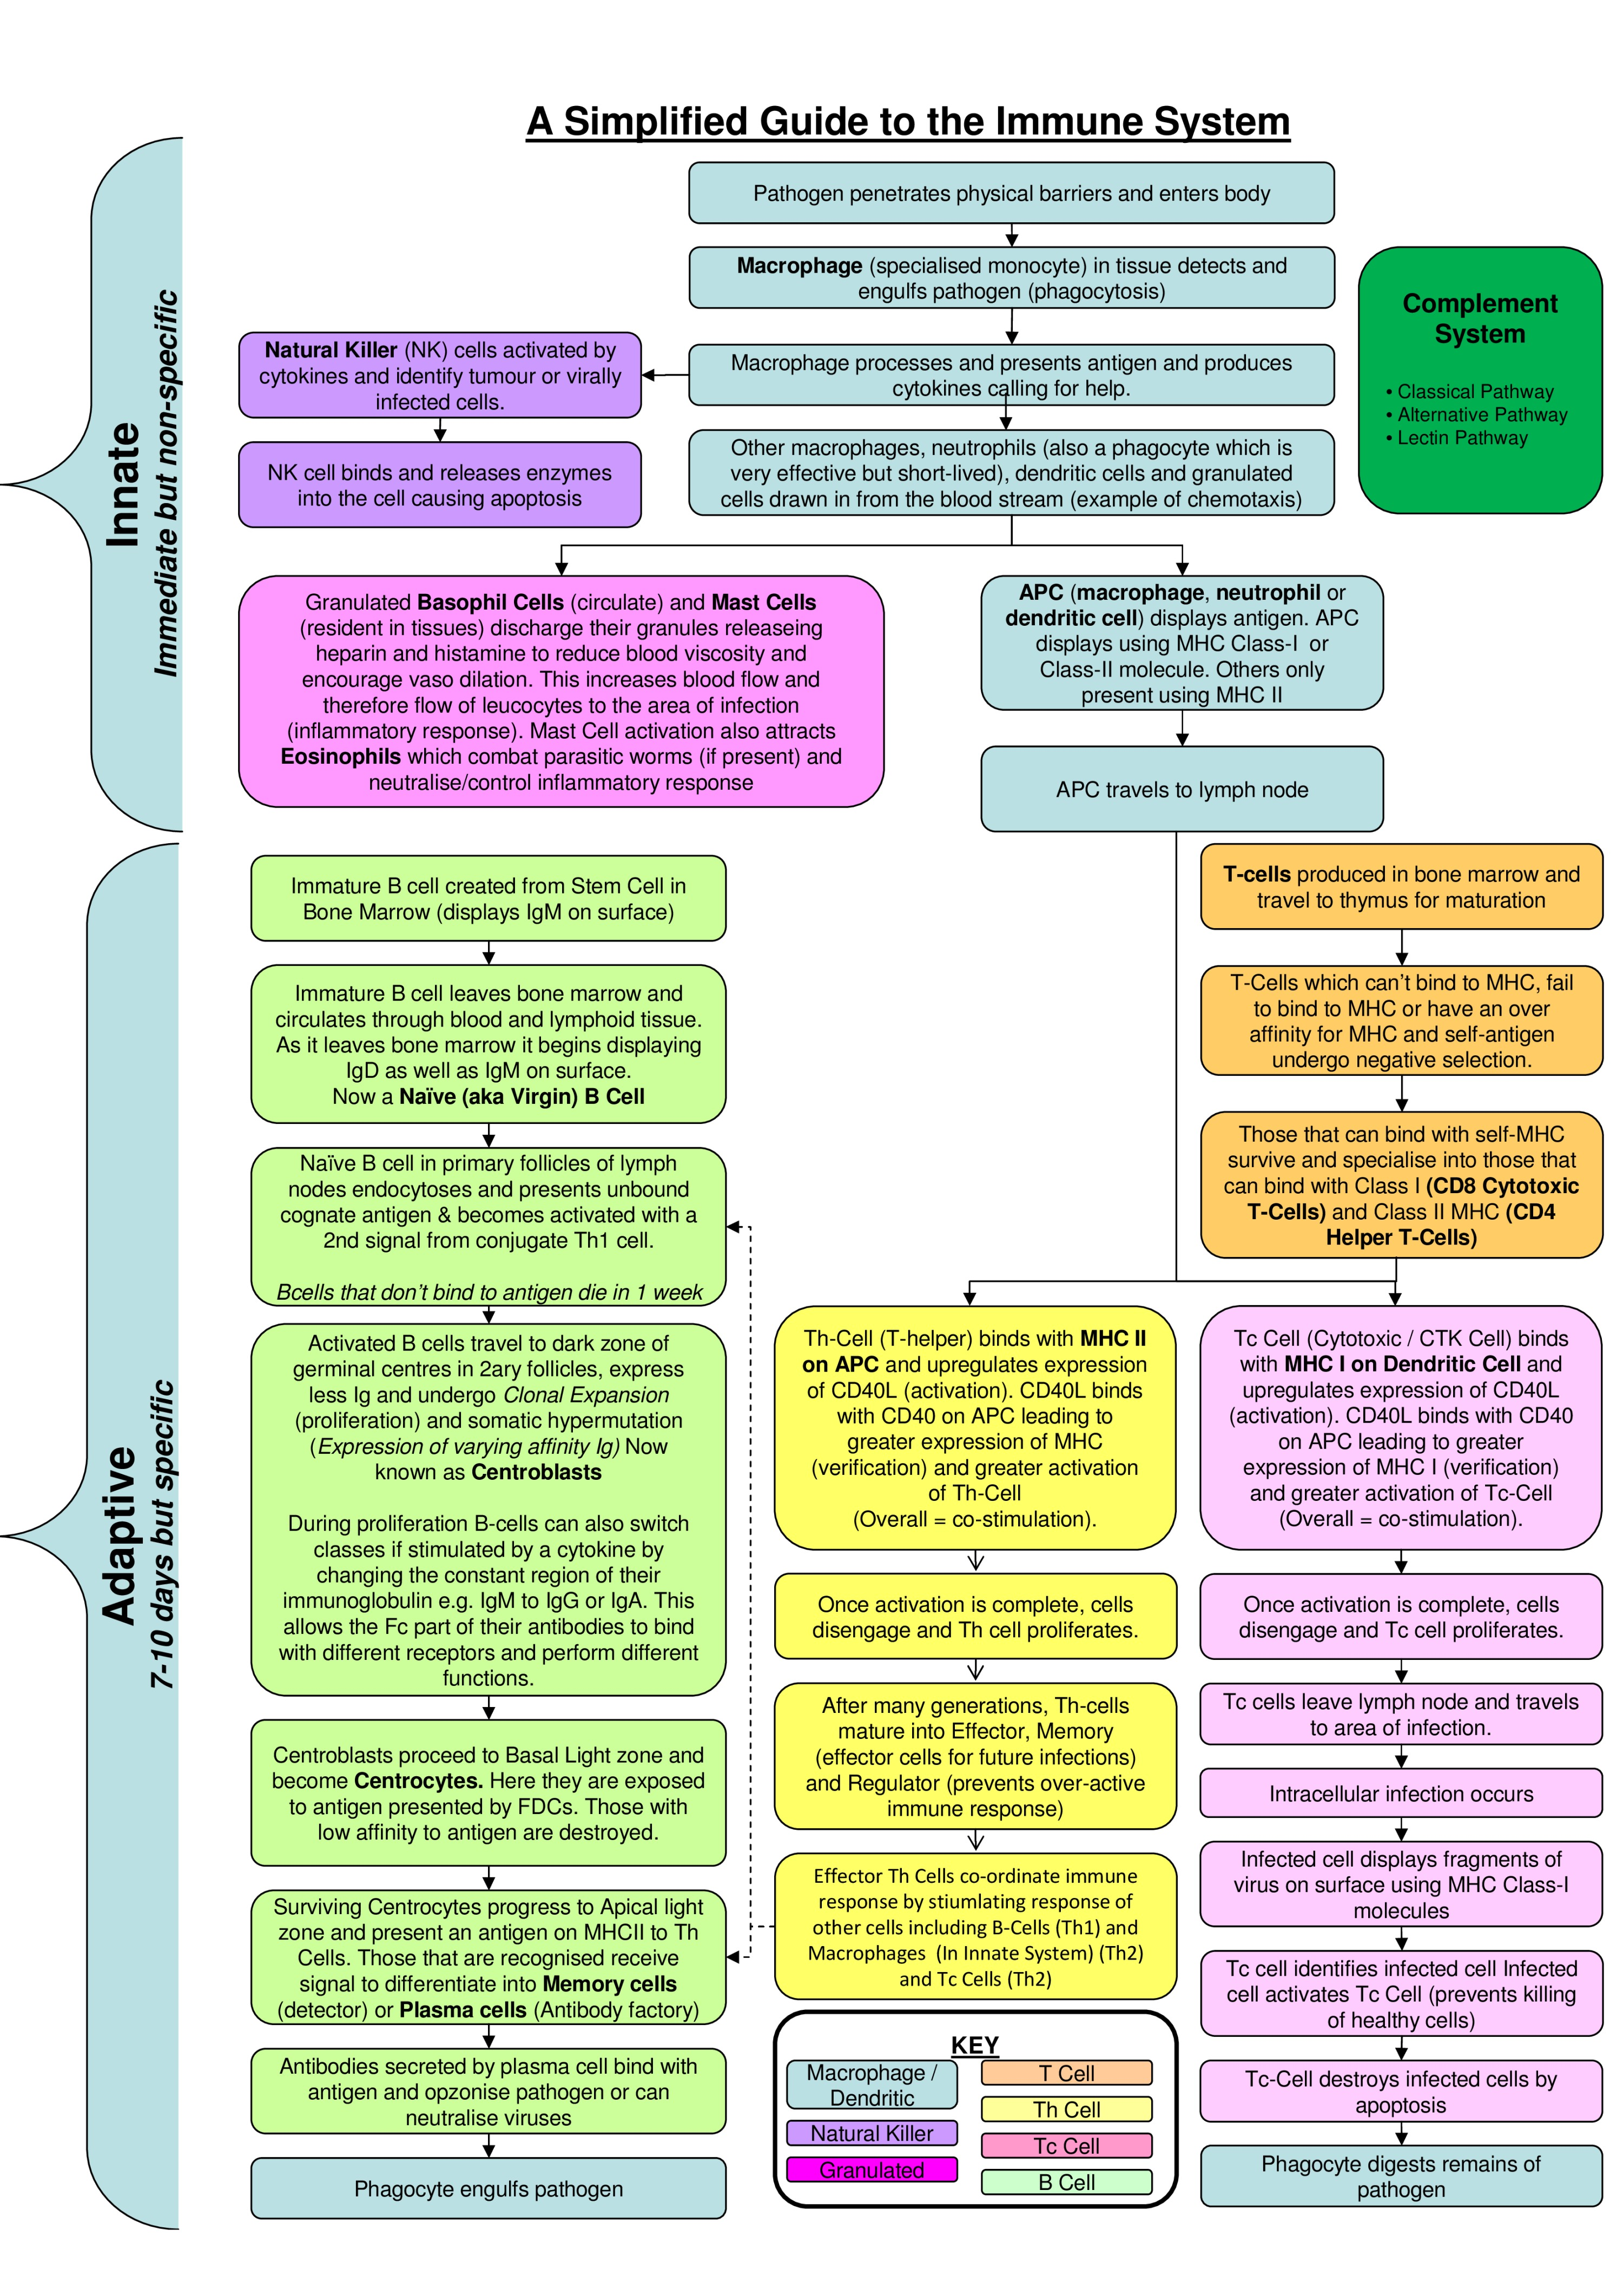
\includegraphics[width=0.85\textwidth]{imunita.jpg}
    \centering
    \label{}
\end{figure}


\subsubsection{Granulocyty} \label{Granulocyty}


\begin{myItemize}[nosep]
    \item terminálně diferenciované nedělící se buňky
    \item polymorfonukleární leukocyty (velmi proměnlivé, polymorfní jádro)
    \item obsahují granula, což jsou obarvitelné částice
    \item \si{12} až \si{15 \mu m}
    \item schopné pohybu
    \item neutrofily
\begin{myItemize}[nosep]
    \item fagocytují, zabíjejí a tráví bakterie
    \item barví se neutrálními barvivy (do růžova)
\end{myItemize}

    \item bazofily
\begin{myItemize}[nosep]
    \item při alergické reakci sekretují histamin a serotonin
    \item barví se zásaditými barvivy (do tmavě modra)
\end{myItemize}

    \item eozinofily
\begin{myItemize}[nosep]
    \item likvidují mnohobuněčné parazity
    \item barví se kyselými barvivy (do červena)
\end{myItemize}

\end{myItemize}



\paragraph{Neutrofily}
\begin{myItemize}[nosep]
    \item polymorfonukleární leukocyty, dříve zvané mikrofágy
    \item 60--70\%  bílých krvinek
    \item mají segmentované jádro
\begin{myItemize}[nosep]
    \item nezralé má tvar podkovy
    \item čím starší, tím více segmentů (až 7)
\begin{myItemize}[nosep]
    \item hypersegmentované buňky
\end{myItemize}

    \item běžně je složeno z 2--5 laloků spojených můstky
    \item ženy mají na jednom segmentu paličkovitý přívěšek, který obsahuje inaktivovaný chromozom X
\end{myItemize}

    \item krátce žijící buňky (v krvi 6-7 dní, ve vazivu 1-4 dny)
    \item přichází v první vlně buněk do místa zánětu
    \item mohou být rychle nahrazeny z kostní dřeně
\end{myItemize}



\paragraph{Neutrofilní aktivita}
\begin{myItemize}[nosep]
    \item receptory neutrofilů jsou schopny rozeznat např. bakterie, které poté fagocytují a ve fagozomech zlikvidují
    \item jejich fagocytická aktivita může být dále stimulována
\begin{myItemize}[nosep]
    \item nízkoafinními Fc receptory na neutrofilech
    \item označením bakterie protilátkami, tzv. \emph{opsonizací}
\end{myItemize}

    \item látky pro rozklad bakterií
\begin{myItemize}[nosep]
    \item superoxidové anionty
    \item peroxid vodíku
    \item chlornanové kationty
\end{myItemize}

    \item mrtvé neutrofily + bakterie + natrávený materiál -> hnis
\end{myItemize}



Zvýšené množství neutrofilů v krvi (neutrofilie) tedy může značit infekci, a to akutní i chronickou.

\begin{description}
\item[Multivalentní antigen]\hfill \\
Struktura obsahující větší množství vazebných míst pro protilátku.

\end{description}


\paragraph{Bazofily}
\begin{myItemize}[nosep]
    \item tvoří 1\% krevních leukocytů
    \item na povrchu jsou receptory pro protilátky (imunoglobuliny E, IgE)
    \item při zvýšené hladině bazofilů v krvi se zvyšuje pravděpodobnost alergické reakce
    \item jsou schopny degranulace
\begin{myItemize}[nosep]
    \item granula splynou s membránou a vylijí se do okolního prostředí
    \item ničí cizí struktury
\end{myItemize}

    \item exocytóza je regulovaná vazbou antigenu na IgE, který je navázaný na IgE receptorech
\begin{myItemize}[nosep]
    \item vysokoafinní IgE receptor váže IgE i pokud není navázaný na antigen ( z čehož, hádám, plynou problémy s alergickou reakcí)
\end{myItemize}

    \item pokud se v těle vyskytne multivalentní antigen, dojde k agregaci receptorů
\begin{myEnumerate}[nosep]
    \item aktivace signalizační kaskády
    \item degranulace granulí
    \item vylití biologicky aktivních aminů (histamin, serotonin)
\end{myEnumerate}

\end{myItemize}



\paragraph{Eozinofily}
\begin{myItemize}[nosep]
    \item 2-4\% leukocytů
    \item mají dvojlaločná jádra
    \item granula (cca 200 na buňku)
\begin{myItemize}[nosep]
    \item hlavní složku tvoří MBP (major basic protein)
\begin{myItemize}[nosep]
    \item má antiparazitickou funkci
    \item aktivuje neutrofily, stimuluje žírné buňky
\end{myItemize}

    \item enzymy histamináza a arylsulfatáza
\begin{myItemize}[nosep]
    \item rozkládají histamin a leukotrieny
    \item mohou tlumit účinek basofilů a žírných buněk
\end{myItemize}

\end{myItemize}

\end{myItemize}



\paragraph{Eozinofilie}
\begin{myItemize}[nosep]
    \item ukazuje na  alergické reakce a parazitární infekce (např. helmintózy)
    \item při napadení organismu patogenem se počet eozinofilů drasticky zvedne
\begin{myItemize}[nosep]
    \item jejich počet se dá snížit kortikoidy
\end{myItemize}

\end{myItemize}



\subsubsection{Agranulocyty} \label{Agranulocyty}


\begin{myItemize}[nosep]
    \item nejsou obarvitelné
    \item monocyty (\si{4e8} na litr)
\begin{myItemize}[nosep]
    \item diferenciují se v makrofágy, dendritické buňky a osteoklasty
\begin{myItemize}[nosep]
    \item makrofágy
\begin{myItemize}[nosep]
    \item fagocytují parazity a vlastní poškozené a apoptotické buňky
    \item produkují oxidační produkty
    \item některé se mění na dendritické buňky
\end{myItemize}

    \item dendritické buňky
\begin{myItemize}[nosep]
    \item fagocytují na periferii, kde migrují do uzlin a prezentují antigeny prostřednictvím MHC II
\end{myItemize}

    \item osteoklasty
\begin{myItemize}[nosep]
    \item odbourá­va­jí kost­ní tkáň
\end{myItemize}

\end{myItemize}

\end{myItemize}

    \item lymfocyty (\(3 \cdot 10^8\) na litr)
\end{myItemize}



\begin{description}
\item[Fagocytární systém]\hfill \\
Soubor všech makrofágů v různých tkáních.


\item[MHC II]\hfill \\
Krátké úseky glykoproteinů (exogenní peptidy sic), které jsou charakteristické pro pohlcenou látku.

\end{description}


\paragraph{Monocyty}
\begin{myItemize}[nosep]
    \item největší krvinky
    \item součástí myeloidní linie
    \item oválné jádro, podkovovité nebo ledvinovité
    \item prekurzory mononukleárního fagocytárního systému
    \item před vstupem do tkáně osm hodin kolují v krvi
    \item prakticky nefunkční, v krvi mají jen funkci "zásobárny makrofágů"
    \item diferenciují na makrofágy a dendritické buňky
\begin{myItemize}[nosep]
    \item na makrofágy diferenciují po vstupu do tkáně kapilární stěnou
\end{myItemize}

\end{myItemize}



\paragraph{Makrofágy}
\begin{myItemize}[nosep]
    \item provádí endocytózu tkáňového debrisu včetně apoptotických tělísek
    \item na povrchu nesou MHC II. třídy
\begin{myItemize}[nosep]
    \item toto MHC kontrolují Th-lymfocyty, které případně spouštějí imunologický poplach, čímž upozorní B-lymfocyty
\end{myItemize}

    \item při zánětu nastupují po neutrofilech
\end{myItemize}



\paragraph{Dendritické buňky}
\begin{myItemize}[nosep]
    \item aktivita
\begin{myEnumerate}[nosep]
    \item endocytují cizorodou látku
    \item přesunou se do mízní uzliny
    \item naštěpí endocytovanou látku a prezentují ji na povrchu
    \item Th-lymfocyt ji potenciálně rozpozná, aktivuje se a vyvolá imunitní reakci
\end{myEnumerate}

    \item in vitro připravíme izolací z krve a použitím interleukinu-4a GM-CSF (granulocytární makrofágový colony stimulating factor)
\end{myItemize}



\paragraph{Osteoklasty}
\begin{myItemize}[nosep]
    \item kostní buňky odbourávající kostní tkáň
    \item vznikají splynutím monocytů => jsou mnohojaderné
    \item funkce např. prořezávání zubů
\begin{myItemize}[nosep]
    \item proti špičce zubu se nachází speciální populace osteoklastů
    \item je třeba odbourat kost čelisti, aby se mohl zub prořezat ven
\end{myItemize}

    \item poruchy v myeloidní linii (především ve funkci monocytů a jejich diferenciačních produktů) mohou mít velký vliv na remodelaci kostní hmoty
\begin{myItemize}[nosep]
    \item Pagetova choroba: nadměrné odbourávání kosti a následné tvoření kosti neplnohodnotné
\end{myItemize}

\end{myItemize}



\paragraph{Lymfocyty}
\begin{myItemize}[nosep]
    \item tvoří 30\% leukocytů
    \item různorodá velikost (\si{5} až \si{15 \mu m})
\begin{myItemize}[nosep]
    \item rozdíl v množství cytoplazmy (většina je zcela vyplněna jádrem)
\end{myItemize}

    \item schopny aktivního pohybu (z krve do tkání --- do místa zánětu nebo do mízní uzliny)
    \item schopny vytvářet mnohočetná komplikovaná mezibuněčná spojení
\begin{myItemize}[nosep]
    \item interakce vícero párů membránových receptorů a jejich ligandů
    \item regulace diferenciace (případně následné proliferace) a efektorové funkce (např. zabití cílové buňky cytotoxickým Tc-lymfocytem)
\end{myItemize}

\end{myItemize}



\paragraph{T-lymfocyty}
\begin{myItemize}[nosep]
    \item vznikají v kostní dřeni, dozrávají v thymu (brzlíku)
    \item tvoří 90\% leukocytů
    \item dělení podle povrchových koreceptorů pro MHC glykoproteiny
\begin{myItemize}[nosep]
    \item CD4 (interakce s MHC II): pomocné (Th) a supresorové
    \item CD8 (interakce s MHC I): cytotoxické (Tc)
\end{myItemize}

    \item dělení podle genů, které byly přestavěny ve funkční T-receptor
\begin{myItemize}[nosep]
    \item rekombinací v nich vznikají nové geny a jsou syntetizovány nové proteiny
\begin{myItemize}[nosep]
    \item přeskupování genových segmentů je prováděno rekombinázami
\end{myItemize}

    \item \(\alpha\)\(\beta\)
\begin{myItemize}[nosep]
    \item výběr genů probíhá náhodně
    \item jsou připraveny na cokoli
\end{myItemize}

    \item \(\gamma \delta\)
\begin{myItemize}[nosep]
    \item výběr genů probíhá na základě evoluce
    \item jedná se o konkrétní poskládání genových segmentů, která jsou nejčastěji používaná a mají smysl
\end{myItemize}

    \item organismy se liší v poměru \(\alpha\)\(\beta\) a \(\gamma \delta\)
\begin{myItemize}[nosep]
    \item např. člověk 95:5, přežvýkavci 70:30
\end{myItemize}

\end{myItemize}

\end{myItemize}



\paragraph{Chyby při vzniku T-lymfocytů}
\begin{myItemize}[nosep]
    \item popletení substrátu; dojde ke spojení ramen dvou chromozomů, které spolu fyzicky vůbec nesouvisí
    \item např. filadelfský chomozom
\begin{myItemize}[nosep]
    \item je na něm fúzní chimérní gen (propojení částí genů Cbl a Abl)
    \item vznik nedeaktivovatelné kinázy schopné transformovat postiženou buňku v buňku nádorovou
\end{myItemize}

\end{myItemize}



\paragraph{B-lymfocyty}
\begin{myItemize}[nosep]
    \item tvoří 5\% leukocytů
    \item produkují protilátky
    \item afinitní maturace
\begin{myEnumerate}[nosep]
    \item když se organismus setká s nějakým antigenem, vylepší svoje protilátky
    \item sekundární odpověď zahrnuje protilátky s vyšší afinitou k antigenu
    \item imunoglobulinové geny náhodně mutují, B-lymfocyty s mutovanými geny poté soupeří o navázání antigenu
    \item ty s nízkou afinitou jsou odstraněny a tak zůstanou pouze ty s vysokou
\end{myEnumerate}

\end{myItemize}



\paragraph{Efektorové buňky}
\begin{myItemize}[nosep]
    \item kategorie buněk tvořená zčásti buňkami ze skupiny T-lymfocytů a zčásti buňkami B-lymfocytů
\begin{myItemize}[nosep]
    \item z T-lymfocytů jsou to pomocné (Th) a cytotoxické (Tc) buňky
    \item z B-lymfocytů jsou to plazmatické buňky, neboli buňky produkující velké množství protilátek
\end{myItemize}

    \item jsou diferenciovány a aktivovány pro výkon své funkce
\end{myItemize}



\paragraph{NK buňky}
\begin{myItemize}[nosep]
    \item tvoří 5\% leukocytů
    \item ničí buňky bez MHC I (rakovinotvorné...), jsou součástí nespecifická imunita
    \item proděraví buňce buněčnou stěnu perforinem
    \item při špatné funkci chronický únavový syndrom
\end{myItemize}




\paragraph{Zánět}
\begin{myItemize}[nosep]
    \item zvýšení průtoku v místě rány
    \item makrofágy, mastocyty a basofily vypouští histamin
\begin{myItemize}[nosep]
    \item zvýšení propustnosti cév (aby se bílé krvinky odstaly lépe na místo zánětu)
    \item prosak krevní plazmy
    \item otok
\end{myItemize}

    \item makrofágy začnou uvolňovat chemoki(ni)ny
\begin{myItemize}[nosep]
    \item lákají další bílé krvinky
    \item stimulují basofily k vylití hydrolytických enzymů
\end{myItemize}

    \item poškozené buňky vylučují prostaglandiny
\begin{myItemize}[nosep]
    \item označují buňku pro Tc-lymfocyt, který v ní po nalezení spustí buněčnou smrt
\end{myItemize}

\end{myItemize}



\subsection{Krevní destičky} \label{Krevní destičky}


\begin{myItemize}[nosep]
    \item nejsou to buňky, ale bezjaderné diskovité útvary
    \item velikost 3 mikrometry
    \item vznikají fragmentací polyploidních megakaryocytů sídlících v kostní dřeni
\begin{myItemize}[nosep]
    \item megakaryocyt vysílá výběžky přes stěny do kapilár a odštěpuje destičky přímo do krve
\begin{myItemize}[nosep]
    \item jeho rozpad je programovanou buněčnou smrtí, zbytky poté uklidí makrofágy
\end{myItemize}

    \item za den jich z jednoho karyocytu vznikne až 100 000
\end{myItemize}

    \item v krvi přežijí 10 dní
    \item neopouští krevní řečiště
\end{myItemize}



\paragraph{Stavba}
\begin{myItemize}[nosep]
    \item regulátory srážení krve
\begin{myItemize}[nosep]
    \item PDGF (platelet derived growth factor)
\begin{myItemize}[nosep]
    \item jako diferenciační faktor epiteliálních buněk se podílí na efektivní reparaci poškozené tkáně
\end{myItemize}

    \item serotonin
\begin{myItemize}[nosep]
    \item vasokonstriktor
    \item jeho uvolnění je stimulováno vazbou na poškozené cévní stěny
    \item schopen uzavřít i malé arterie
\end{myItemize}

\end{myItemize}

\end{myItemize}



\paragraph{Průběh opravy poškozené tkáně}
\begin{myEnumerate}[nosep]
    \item destička se dostane do kontaktu s kolagenními vlákny
    \item nastane exocytóza faktorů aktivujících ostatní destičky
    \item dojde k uvolnění aktivačních látek ze stěn poškozených cév
\begin{myItemize}[nosep]
    \item změna protrombinu na trombin
\end{myItemize}

    \item trombin katalyzuje přeměnu fibrinogenu na fibrin
    \item fibrin polymeruje a vytváří vláknitou síťovinu vznikající krevní sraženiny
    \item vznik trombu (sraženiny)
\end{myEnumerate}



\subsection{Patologie} \label{Patologie}


\paragraph{Leukémie}
\begin{myItemize}[nosep]
    \item rakovina krve
    \item dochází k nádorové přeměně některého z diferenciačních stádií buněk odvozených od kmenových buněk kostní dřeně
    \item zvýšený počet leukocytů jednoho typu v krvi
\begin{myItemize}[nosep]
    \item myeloblastické zvýšení
\begin{myItemize}[nosep]
    \item zvýšené množství granulocytů a monocytů
\end{myItemize}

    \item lymfoblastické zvýšení
\begin{myItemize}[nosep]
    \item zvýšené množství lymfocytů
\end{myItemize}

    \item obě mohou být akutní nebo chronická
\end{myItemize}

    \item leukocyty nedozrávají, jsou nefunkční
    \item rizikové faktory
\begin{myItemize}[nosep]
    \item kouření
    \item chemikálie (benzen)
    \item radioaktivní záření
    \item léčba jiného nádorového onemocnění
    \item filadelfský chromozom
\end{myItemize}

    \item efektivní řešení: chemoterapie a transplantace kostní dřeně
\end{myItemize}



\paragraph{Mononukleóza}
\begin{myItemize}[nosep]
    \item EBV virus napadá B-lymfocyty, nebo jejich prekurzory
\begin{myItemize}[nosep]
    \item B-lymfocyty se pomnoží, tváří se jako cizí organismus a tělo se brání
    \item dochází k narušení rovnováhy mezi jednotlivými složkami imunitního systému
\end{myItemize}

    \item po vyléčení máme EBV na celý život
\end{myItemize}



\section{Lymfatický systém} \label{Lymfatický systém} \FloatBarrier


Lymfatické i lymfoidní tkáně jsou všude po těle, zejména v místech, kde do těla vstupují patogeny, nebo kudy během infekce putují.

\begin{description}
\item[MALT]\hfill \\
Lymfoidní tkáň asociovaná s mukózou (sliznicí).


\item[GALT]\hfill \\
Lymfoidní tkáň asociovaná se střevem (gut).


\item[BALT]\hfill \\
Lymfoidní tkáň asociovaná s dýchacími cestami (bronchy).

\end{description}


\begin{figure}
    \caption{Schematický obrázek mízní uzliny}
    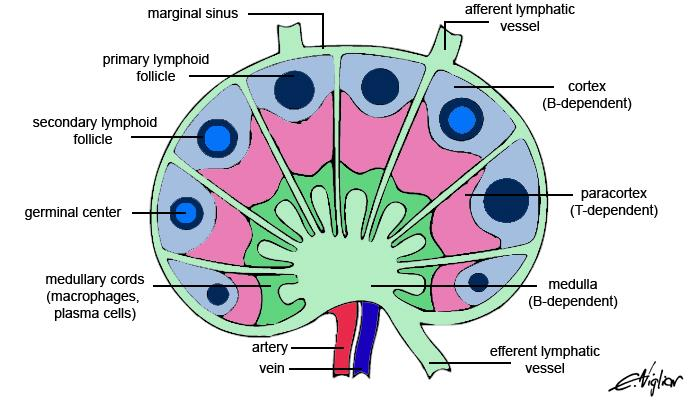
\includegraphics[width=0.85\textwidth]{uzlina.jpg}
    \centering
    \label{}
\end{figure}


\paragraph{Lokalizace lymfatických cest}
\begin{myItemize}[nosep]
    \item pod epitely (lymfoidní tkáň asociovaná s epitely)
\begin{myItemize}[nosep]
    \item místa proliferace a diferenciace lymfocytů
    \item MALT, GALT, BALT
\end{myItemize}

    \item v lymfatických orgánech
\begin{myItemize}[nosep]
    \item anatomicky diferenciovaná množina lymfoidní tkáně
    \item složeny pouze z lymfoidní tkáně
    \item dělení
\begin{myItemize}[nosep]
    \item primární
\begin{myItemize}[nosep]
    \item zajišťují hematopoézu (krvetvorbu)
    \item probíhá v nich selekce lymfocytů, které nereagují s tělěm
    \item kostní dřeň, thymus (brzlík)
\end{myItemize}

    \item sekundární
\begin{myItemize}[nosep]
    \item napojeny na lymfatický i oběhový systém
    \item zajišťují efektivní setkávání buněk imunitního systému a efektivní kompartmentaci imunitního dozoru
    \item slezina, mízní uzliny (schéma mízní uzliny viz obrázek výše)
\begin{myItemize}[nosep]
    \item stromální buňky  jsou velmi důležité
    \item tvoří "lešení" pro hematopoetické buňky
    \item vytváří vhodné prostředí pro setkání lymfocytů s antigeny
\end{myItemize}

\end{myItemize}

\end{myItemize}

\end{myItemize}

\end{myItemize}



\begin{description}
\item[totipotentní buňka]\hfill \\
Někdy též \emph{omnipotentní} buňka --- buňka schopná vytvořit jakýkoli jiný druh buňky, ergo celý organismus. Takovými buňami jsou zygoty a dělivé meristémy.


\item[multipotentní buňka]\hfill \\
Buňka schopná diferenciace do mnoha typů buněk, pouze však v rámci jedné tkáně. Příkladem mohou být kmenové buňky.

\end{description}


\paragraph{Kostní dřeň}
\begin{myItemize}[nosep]
    \item veliký orgán
    \item sídlo hematopoézy, dochází zde k proliferaci buněk obou hematopoetických linií (lymfoidní i myeloidní)
    \item dělení podle barvy
\begin{myItemize}[nosep]
    \item červená kostní dřeň
\begin{myItemize}[nosep]
    \item hematopoetická
    \item u fetu probíhá krvetvorba jen v játrech a slezině
    \item po narození je v těle pouze červená k.d. a hematopoéza probíhá výhradně tam
    \item v dopělosti pouze v plochých kostech a obratlích
\end{myItemize}

    \item žlutá kostní dřeň
\begin{myItemize}[nosep]
    \item tuková
\end{myItemize}

    \item šedá kostní dřeň
\end{myItemize}

    \item 0,1\% buněk kostní dřeně má na povrchu membránový protein CD34
    \item každý buněčný typ je nezávisle regulován
\begin{myItemize}[nosep]
    \item erytropoetin (EPO), kolonie stimulující faktory (CSF)
\end{myItemize}

    \item kmenové buňky v kostní dřeni
\begin{myItemize}[nosep]
    \item stačí transplantovat 5000 buněk pro zajištění kompletní krvetvorby (<= myší model)
\end{myItemize}

    \item typickou markerovou molekulou je C-kit CD117
\begin{myItemize}[nosep]
    \item je na povrchu buňky
    \item obsahuje informace o buněčném typu, stádiu diferenciace a buněčné aktivitě
\end{myItemize}

\end{myItemize}



Hematopoéza se dá jednoduše sledovat in vitro. Nejprve se provede výplach z kostní dřeně (jako na praktikách), poté se nechají jednotlivé buňky růst na agaru. Vzniknou nepohyblivé kolonie, které se dají dobře pozorovat.

\paragraph{Embryonální krvetvorba}
\begin{myItemize}[nosep]
    \item vzniká cca třetí týden
\begin{myItemize}[nosep]
    \item ze žloutkového vaku se vytvoří krevní ostrůvky obsahující primitivní erytroblasty
    \item větší než ty dospělé, mají jiný hemoglobin (Hb) a obsahují jádro
\end{myItemize}

    \item od pátého týdne vzniká intraembryonální krvetvorba
\begin{myItemize}[nosep]
    \item v játrech, slezině, kostní dřeni
\end{myItemize}

\end{myItemize}



\chapter{Svaly} \label{Svaly}


\begin{myItemize}[nosep]
    \item účastní se \textbf{cytokinese}
\begin{myItemize}[nosep]
    \item proces je zprosdředkovaný aktino-myozinovým komplexem 26
    \item aktinová vlákna omotána okolo buněk epitelu, ukotvena v adhezivních spojích
    \item pomocí pohybu myozinu se změní jejich tvar, dojde k lokálnímu zaškrcení buňky
    \item dojde k deformaci celé buněčné vrstvy
\end{myItemize}

    \item celý epitel funguje jako jedna signalizační a morfologická jednotka
    \item aktinová vlákna jsou antiparalelně uspořádána a ukotvena do kotvících struktur (Z disky)
    \item čtyři typy svalových buněk: kosterní svaly, srdeční svaly, hladké svaly, myoepiteliální buňky
\end{myItemize}



\todo{Doplnit a upravit celou sekci.}

\section{Kosterní svaly} \label{Kosterní svaly} \FloatBarrier


\begin{myItemize}[nosep]
    \item specializace na ohyb kostry a spojení pák (kosti, chrupavky)
    \item pohyby ovládané vůlí, někdy i mimovolné (svalový třes)
    \item rychlost ovládání je zajištěna inervací volným nervstvem
\begin{myItemize}[nosep]
    \item okamžitá reakce pák a protipák je nutná např. k řeči
\end{myItemize}

    \item každý sval by měl fungovat jako mechanická jednotka
\begin{myItemize}[nosep]
    \item to zajišťuje soustava vazivových pochev
\end{myItemize}

\end{myItemize}



Svaly vznikají z myoblastů, které jsou určeny expresí genů z rodin MyoD a MEF2.

\paragraph{Vznik}
\begin{myEnumerate}[nosep]
    \item proliferace
    \item diferenciace
    \item splynutí myoblastů ve svalová vlákna
\begin{myItemize}[nosep]
    \item myoblasty se už nikdy nedělí ani nereplikují DNA
    \item z toho plyne ztížená regenerace svalu
\end{myItemize}

\end{myEnumerate}



\begin{figure}
    \caption{Schematický obrázek svalových vláken}
    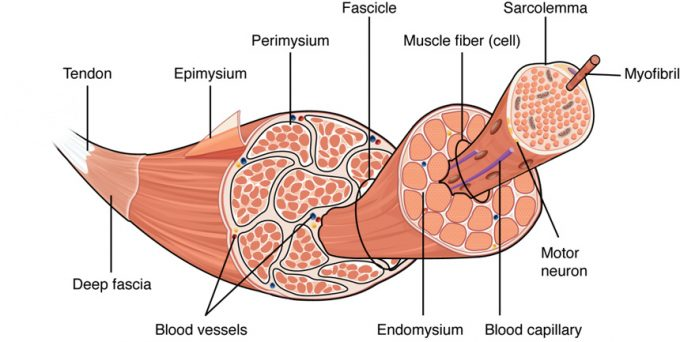
\includegraphics[width=0.85\textwidth]{sval.jpg}
    \centering
    \label{}
\end{figure}


\paragraph{Stavba}
\begin{myItemize}[nosep]
    \item některé kosterní svalové buňky jsou velmi velké, je potřeba vícejadernost
    \item často splyne více myocytárních buněk a vznikne \emph{syncytium}
    \item jsou \si{3cm} dlouhé a mají \si{100 \mu m} v průměru
    \item tvoří svalová vlákna
    \item obaly
\begin{myItemize}[nosep]
    \item endomysium: jemná vrstva vaziva obalující každé svalové vlákno
    \item perimysium: vazivová pochva obalující svazky (\(=\) snopce, fascia) svalových vláken
    \item epimysium: obal celého svalu
\end{myItemize}

    \item velice důležitá je inervace svalu
\begin{myItemize}[nosep]
    \item mechanická odolnost nervu je zajištěna mezibuněčnaou hmotou
\end{myItemize}

    \item svalová hmota se zvětšuje narůstáním aktinomyozinových vláken v už existujících svalových jednotkách
    \item příčné svaly interagují s pojivovou tkání, musí tedy být ukotveny na kosti
\begin{myItemize}[nosep]
    \item k tomu slouží šlachy: struktury s orientovanými kolagenními vlákny, které jsou syntetizovány fibroblasty
\end{myItemize}

\end{myItemize}



\begin{figure}
    \caption{Detailní schéma stavby sarkomery}
    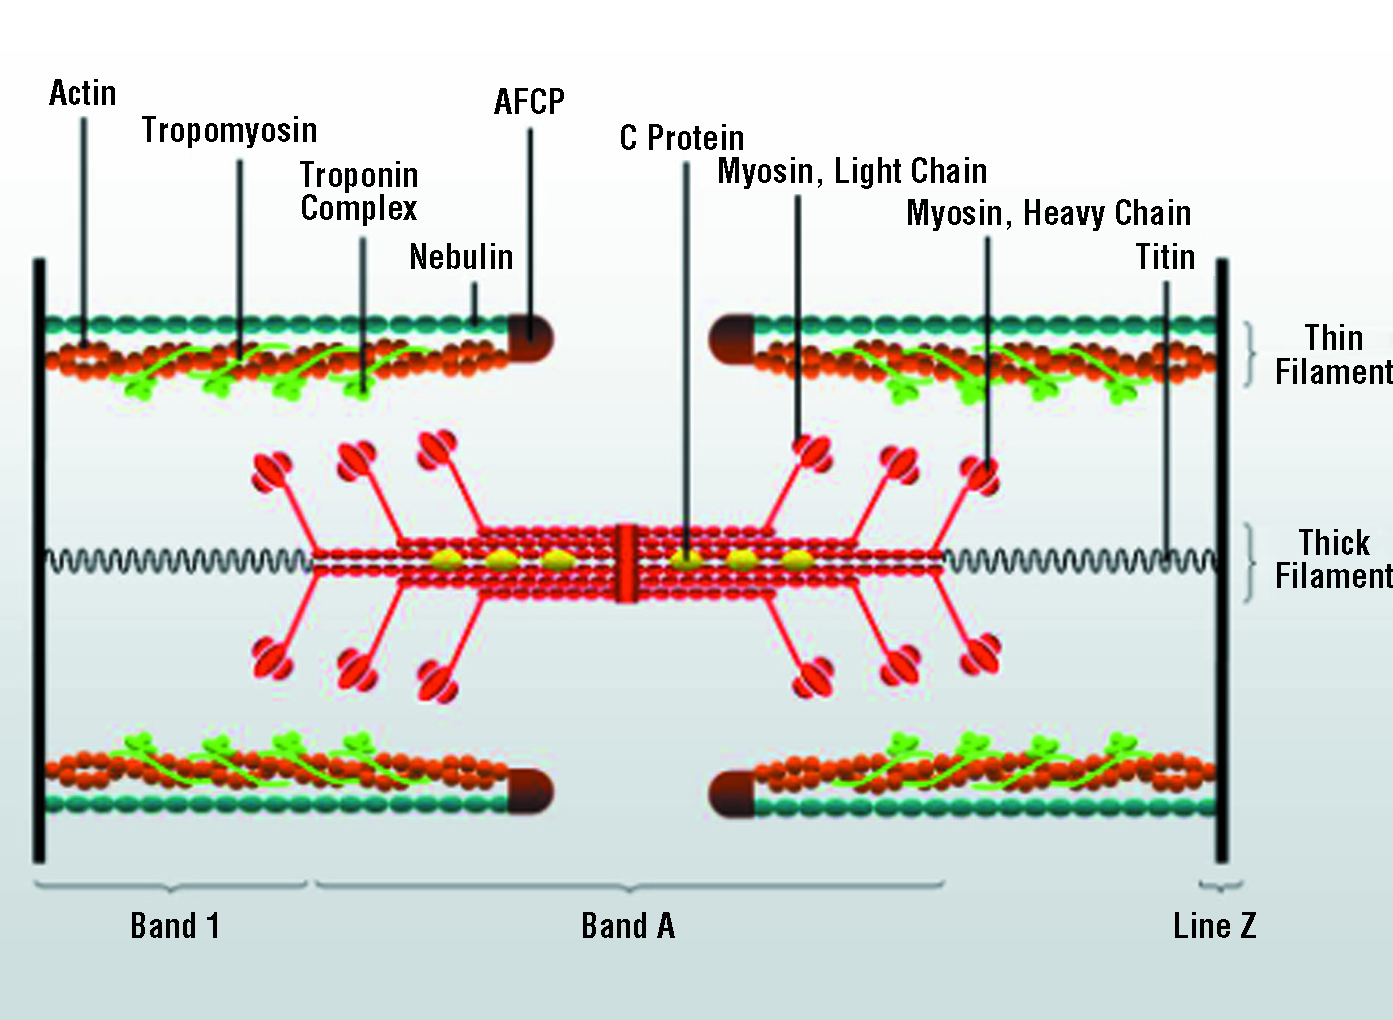
\includegraphics[width=0.85\textwidth]{sarkomera.jpg}
    \centering
    \label{}
\end{figure}


\begin{description}
\item[svalové vřeténko]\hfill \\
Specializovaná struktura podávající informaci o napnutosti či relaxovanosti svalu do CNS.

\end{description}


\paragraph{Svalová vřeténka}
\begin{myItemize}[nosep]
    \item někdy probíhá specializace do mnohobuněčných syncytiálních útvarů se senzorickou funkcí místo mechanické, vznikají deriváty svalu, \emph{svalová vřeténka}
    \item jsou zde intimní propojení senzorických nervových zakončení s něčím svalového původu
    \item signál o deformaci těchto svalů se přenáší do mozku, který tím získává zásadní informace o "zapnutí" našich svalů
\begin{myItemize}[nosep]
    \item pokud tato signalizace nefunguje, mozek nedokáže synchronizovat naše pohyby
\end{myItemize}

\end{myItemize}



\paragraph{Svalové kmenové buňky}
\begin{myItemize}[nosep]
    \item i v diferenciovaných příčně pruhovaných svalech máme kmenové buňky pro příčně pruhované svaly, tzv. \emph{satelitní buňky}
    \item jsou pod pojivem na povrchu svalu, je jich málo, mají omezenou činnost
    \item aktivují MyoD
\end{myItemize}



\paragraph{Svalová aktivita}
\begin{myItemize}[nosep]
    \item depolarizace membrány díky aktivitě Na/K ATPázy
    \item ve svalové buňce musí fungovat vápenaté pumpy => aktivní transport Ca2+ do ER - troponin-tropomyozinový komplex brání myozinu pohybovat se po aktinu
    \item po navázání komplexu na Ca2+ změní konformaci => myozinové hlavy můžou běžet po aktinu - pro mechanické vlastnosti důležité pospojování struktur => fungování jako 1 mechanická jednotka
    \item proužkování svalu
= linie, na které se napojuje aktinový cytoskelet v hexagonálním uspořádání
    \item ve všech volných dírách mezi aktinovými hexagony hexagonální myozinové hlavice - klíčový protein aktinin
30
    \item vyrůstá ze Z-disku jako krystalizační jádro = místo s pevným připojením aktinu - uvnitř buňky v jednom svalovém vlákně vytváří sarkomery několik soustav vedle sebe
    \item propojení subvláken díky intermediálním filamentům (molekuly desminu)
\end{myItemize}



\subsection{Svalové proteiny} \label{Svalové proteiny}


\todo{Detailněji popsat mechanismus práce svalu.}

\paragraph{Myosin}
\begin{myItemize}[nosep]
    \item jediný protein tlustých vláken (myofibril)
    \item z celkového proteinu svalu tvoří 60-70\%
    \item molekulová hmotnost 540 000
    \item tvořen 6 řetězci (dva těžké + čtyři lehké)
\begin{myItemize}[nosep]
    \item těžké jsou vzájemně uspořádané do dvoušroubovice o délce 150nm, mají globulární N-terminální konce
\end{myItemize}

\end{myItemize}



\paragraph{Troponin-tropomyozinový komplex}
\begin{myItemize}[nosep]
    \item molekulová hmotnost 72 000
    \item skládá ze tří podjednotek
\begin{myItemize}[nosep]
    \item troponin C
\begin{myItemize}[nosep]
    \item váže \(\ce{Ca^{2+}}\)
    \item molekulová hmotnost 18 000
    \item vazba na troponin T
    \item podobný kalmodulinu
\end{myItemize}

    \item troponin I
\begin{myItemize}[nosep]
    \item intermediární, váže se mezi troponiny C a T
\begin{myItemize}[nosep]
    \item vazba na aktin a troponin T
\end{myItemize}

    \item molekulární hmotnost 23 000
    \item inhibuje interakce mezi aktinem a myozinem do doby vazby Ca2+ na troponin C
\end{myItemize}

    \item troponin T
\begin{myItemize}[nosep]
    \item molekulová hmotnost 31 000
    \item vazba na tropomyozin, troponin I a troponin C v místě styku 2 molekul tropomyozinu
\end{myItemize}

\end{myItemize}

\end{myItemize}



\paragraph{Kreatinkináza}
\begin{myItemize}[nosep]
    \item katalyzuje přenos fosfátu z ATP na kreatin, který poté zásobuje svaly velmi rychlou energií
    \item hmotnost 86 000Da
    \item dvě podjednotky, které mohou být dvojího typu (M = muscle, B = brain)
    -> 3 isoenzymy
\begin{myItemize}[nosep]
    \item MM
    \item MB
    \item BB
\end{myItemize}

\end{myItemize}



\paragraph{Aldoláza}
\begin{myItemize}[nosep]
    \item hmotnost 160 000 Da
    \item 3 isoenzymy
\begin{myItemize}[nosep]
    \item A: sval
    \item B: játra
    \item C: mozek
\end{myItemize}

\end{myItemize}



\paragraph{Laktátdehydrogenáza}
\begin{myItemize}[nosep]
    \item hmotnost 135 000 Da
    \item 5 isoenzymů
    \item je ve všech tkáních
    \item různé zastoupení: LD1: srdce, LD2: srdce, LD3: svalstvo atd.
\end{myItemize}



\paragraph{Myoglobin}
\begin{myItemize}[nosep]
    \item hmotnost 18 000 Da
    \item nachází se v červených svalových vláknech
\end{myItemize}



\paragraph{Titin}
\begin{myItemize}[nosep]
    \item pružina relaxující sval
    \item největší známý protein, obsahuje 34 350 AK
\end{myItemize}



\paragraph{Nebulin}
\begin{myItemize}[nosep]
    \item molekulární pravítko určující délku aktinové části sarkomery
\end{myItemize}



\subsection{Inervace} \label{Inervace}


\emph{Viz také \hyperref[Schop­nost re­gen­er­ace]{schopnost regenerace axonů}.}

\paragraph{Perimysium}
\begin{myEnumerate}[nosep]
    \item větvení axonů
    \item rozšířená zakončení na povrchu svalových buněk
    \item motorické ploténky
    \item myoneurální spojení
\end{myEnumerate}



\paragraph{Neurotransmiter (acetylcholin)}
\begin{myEnumerate}[nosep]
    \item po vylití váčků z nervového zakončení v synaptické štěrbině se váže na acetylcholinový receptor
    \item depolarizace membrány svalové buňky
    \item šíří se dovnitř skrz systém příčných T-tubulů
    \item signál je přenesen na sarkoplazmatické retikulum (SR)
\begin{myItemize}[nosep]
    \item membrána T-tubulu je propojena s membránou SR
\end{myItemize}

    \item uvolnění \(\ce{Ca^{2+}}\) z SR do cytoplasmy
    \item kontrakce svalu
\end{myEnumerate}



Svaly jsou příkladem excitatorních buněk: mají nerovnoměrné uspořádání \(\ce{K+}\) a \(\ce{Na+}\) iontů. To napomáhá vedení vzruchu.

\subsection{Regulace stahu příčně pruhovaného svalu} \label{Regulace stahu příčně pruhovaného svalu}


\begin{myItemize}[nosep]
    \item koncentrační gradient mezi SR a cytoplazmou je 10 000
\begin{myItemize}[nosep]
    \item potencuje rychlost vtoku vápenatých iontů do cytoplasmy
\end{myItemize}

    \item kreatin ve svalech
\begin{myItemize}[nosep]
    \item je pomocí enzymu kreatin kinázy fosforyluován na kreatin fosfát
    \item slouží jako zásobní energetický zdroj
\end{myItemize}

\end{myItemize}



\paragraph{Průběh svalového stahu}
\begin{myEnumerate}[nosep]
    \item zvýšení koncentrace iontů \(\ce{Ca^{2+}}\)
    \item deformace troponinu a tropomyozinu
    \item interakce myozinové hlavice s aktinem
    \item stah svalu
\end{myEnumerate}



\paragraph{Složení relaxovaného svalu}
\begin{myItemize}[nosep]
    \item koncentrace ATP 4mM
    \item koncentrace ADP 0,013mM
    \item reakční kinetika posunuta ve směru ATP -> ADP + P
    \item koncentrace kreatinu 13mM
    \item koncentrace kreatin fosfátu 25mM
    \item reakce jde ve směru kreatin fosfát -> kreatin + fosfát
\end{myItemize}



ATP vystačí svalu na 2s aktivity, kreatin fosfát na 8s. Poté dochází už jen odbouránvání organických sloučenin. Anaerobní zdroj energie je glykogen, který je odbouráván na pyruvát a vystačí na 60s. Další ATP je tvořeno glykolýzou, která je 2,5x rychlejší než oxidativní metabolismus.

\subsection{Motorická jednotka} \label{Motorická jednotka}


Jedno nervové vlákno (axon) může inervovat různý počet svalových vláken, která poté tvoří tzv. \textbf{motorickou jednotku}.

\paragraph{Základní informace}
\begin{myItemize}[nosep]
    \item axon se může rozvětvit, pak vznikne nervosvalová ploténka s několika svalovými vlákny
    \item MJ jsou různě velké podle požadavku na typ svalového stahu (v bicepsu větší než na jazyku)
    \item vlákna nejsou schopna stupňované kontrakce
    \item počet axonů na sval se také liší
\begin{myItemize}[nosep]
    \item oční svaly: 1 axon
    \item svaly končetin: 100 a více axonů inervovaných jedním neuronem
\end{myItemize}

    \item designování velikosti MJ probíhá v prenatálním období a do třetího roku života
\end{myItemize}



\subsection{Pomalá a rychlá svalová vlákna} \label{Pomalá a rychlá svalová vlákna}


\begin{myItemize}[nosep]
    \item rychlá vlákna: bílá, málo myoglobinu, anaerobní metabolismus
    \item pomalá vlákna: červená, mnoho myoglobinu, aerobní metabolismus
    \item výskyt konkrétního typu závislý na typu inervace, frekvenci vylévání acetylcholinu, způsobu dráždění svalové buňky, zdroji příslušného nervu
\begin{myItemize}[nosep]
    \item přehozením nervů se dá z bílého udělat červené a naopak
\end{myItemize}

    \item v rámci jednoho svalu různé typy svalových vláken v různé proporci
    \item smíšená vlákna mají znaky obou předchozích typů
\end{myItemize}



\subsection{Růst svalů} \label{Růst svalů}


\begin{myItemize}[nosep]
    \item čím více svalů, tím větší signalizace k menšímu růstu pomocí produkce myostatinu - myostatin = negativní regulátor růstu svalu
\begin{myItemize}[nosep]
    \item receptor nefunguje => přírůstek svalové hmoty
\end{myItemize}

    \item u AIDS zvýšená produkce myostatinu => úbytek svalové hmoty
    \item zvětšení svalové hmoty = zvětšování syncitií => přidělání dalšího systému sarkomer
\end{myItemize}



\subsection{Svalová onemocnění} \label{Svalová onemocnění}


\paragraph{Myasthenia gravis}
\begin{myItemize}[nosep]
    \item autoimunitní
    \item postupující svalová ochablost
    \item B-lymfocyty v brzlíku tvoří protilátky proti acetylcholinovým receptorům
    \item receptor je interalyzován (= endocytován) do buňky => sval neschopen přijímat signál => postupná atrofie
    \item 2. možnost
\begin{myItemize}[nosep]
    \item imunitní systém rozpoznává acetylcholinový receptor jako cizorodou látku
    \item myelic basic protein MBP v CNS
    \item destrukce myelinových pochev díky aktivitě autoreaktivních cytotoxických T-lymfocytů
    \item nelze ovládat postižené svaly => není inervován => atrofuje
\end{myItemize}

\end{myItemize}



\paragraph{Narušení inervace svalu}
\begin{myItemize}[nosep]
    \item po úraze, po narušení páteře
    \item neinervovaný sval atrofuje => zmenšuje se (od určitého stadia nevratně)
    \item možno změnit rychlý sval na pomalý změnou inervace
\end{myItemize}



\paragraph{Svalová dystrofie – myopatie}
\begin{myItemize}[nosep]
    \item poškození svalových vláken nesouvisející s inervací či autoimunitou
    \item nefunkčnost konkrétních enzymů/syndromy patologií mitochondrií
    \item typy
\begin{myItemize}[nosep]
    \item glykogenosy
\begin{myItemize}[nosep]
    \item abnormální ukládání glykogenu ve svalu
    \item dědičné autosomálně recesivní onemocnění
\end{myItemize}

    \item McArdle
\begin{myItemize}[nosep]
    \item chybí myofosforyláza b => svalová slabost, křeče
    \item při cvičení se v plasmě nezvyšuje laktát => nedochází k poklesu pH
\end{myItemize}

    \item Tauri
\begin{myItemize}[nosep]
    \item svalová bolest
    \item chybí fosfofrukokináza => hromadění prekurzorů ve tkáních (glc-6-P, fru-6-P)
\end{myItemize}

    \item Duchennova svalová dystrofie
\begin{myItemize}[nosep]
    \item gonosomálně recesivní onemocnění
    \item chlapci věku 3-7let
    \item nejdříve pánevní pletenec => ramenní pletenec
    \item ve věku 10-12 let končí na vozíku
    \item v séru zvýšeny enzymy (kreatinkináza) dlouho před prvními symptomy
    \item způsobeno mutací genu pro dystrofin
\begin{myItemize}[nosep]
    \item propojuje receptor pro ECM s aktinovým cytoskeletem (vnitřek s vnějškem)
    \item mutace => sval má špatné mechanoelastické vlastnosti => poškození => atrofie
\end{myItemize}

\end{myItemize}

    \item proti acetylcholinovému receptoru se může vytvořit autoimunitní onemocnění
\begin{myItemize}[nosep]
    \item rychlá únava a obrna svalů
        => destrukce receptoru => nemůže přejít neuromuskulární signál
\end{myItemize}

\end{myItemize}

\end{myItemize}



\section{Srdeční svaly} \label{Srdeční svaly} \FloatBarrier


\begin{myItemize}[nosep]
    \item optimalizované pro pomalé, opakované pohyby
    \item nepříliš ovladatelné vůlí
    \item exprese receptorů nastavená tak, aby po srdci běžely vlny signálů => nezbytné vodivé propojení => gap junctions + desmozomy (aby to fungovalo jako 1 mechanická jednotka)
    \item utilizuje široké spektrum látek
\begin{myItemize}[nosep]
    \item glukóza, laktát, ketolátky, aminokyseliny, (ne)esterifikované MK
\end{myItemize}

    \item má příčné pruhování
    \item dobrý elektrický kontakt všech srdečních buněk => vzruch putuje z jednoho vlákna na další
    \item zákon "všechno nebo nic" (idealizovaný případ)
\begin{myItemize}[nosep]
    \item podráždění myokardu v určitém místě => vyvolání akčního potenciálu => rozšíření na celý myokard => kontrakce
\end{myItemize}

\end{myItemize}



\paragraph{Kardiomyocyt}
\begin{myItemize}[nosep]
    \item jednojaderná buňka
    \item centrálně uložené oválné jádro
    \item 40\% mitochondrií, GA, glykogen, lipidy, kontraktilní aparát, SR
    \item 150\(\mu\)m velká
\end{myItemize}



\paragraph{Purkyňova vlákna}
\begin{myItemize}[nosep]
    \item svalové buňky specializované pro přenos signálu po celém srdci
    \item málo myozinu
    \item T-tubuly tlusté a krátké => svalové jednotky jsou menší
\end{myItemize}



\paragraph{Stavba}
\begin{myItemize}[nosep]
    \item "cik cak" desmozomální propojení => trojrozměrné => na základě propojení a orientace lze nastavit způsob stahu celého srdce
    \item tvořená z buněk splanchického mezodermu
    \item není to syncitiální struktura => struktura tvořená individuálními buňkami pevně propojenými desmozomálními spoji a proděravěné gap junctions => zároveň jedna mechanická jednotka i signalizační jednotka
    \item struktura rozvětvených buněk
\begin{myItemize}[nosep]
    \item místa propojení = interkalární disky = hypertrofované desmozomy s gap junctions
\end{myItemize}

    \item specializované kardiomyocyty ke generaci pacemakerové neustále se opakující aktivaci iontových kanálů s konkrétní frekvencí => autonomie srdce v signalizace ke svalové aktivitě
\begin{myItemize}[nosep]
    \item funkce pacemakeru způsobena koordinací součinnosti různých iontových kanálů
    \item tuto aktivitu lze posttranslačně měnit (fosforylací) => zrychlení/zpomalení tepu
    \item endogenní vznik vzruchů (akčních potenciálů) ve specializovaných pacemarkerových buňkách => šíření na     ostatní vlákna
\end{myItemize}

\end{myItemize}



\paragraph{Regenerace srdečního svalu}
\begin{myItemize}[nosep]
    \item špatně regeneruje
    \item nejsou v něm kmenové buňky pro srdce
\begin{myItemize}[nosep]
    \item ale mohou do něj vstupovat a dodiferencovat se do kardiomyocytů
\end{myItemize}

    \item při nedostatečném zásobení srdečního svalu kyslíkem => nekróza tkáně => vznik jizev => narušení přenosu signálu po srdci
\begin{myItemize}[nosep]
    \item velikost jizev ovlivňuje aktivita fibroblastů
\end{myItemize}

    \item pruhováno ve stejném směru jako svalová vlákna
\end{myItemize}



\section{Hladké svaly} \label{Hladké svaly} \FloatBarrier


\begin{myItemize}[nosep]
    \item slouží k k tvorbě pomalých, mimovolných stahů
    \item je na místech, kde je třeba regenerovat, a v místech, kde se tkáň často obměňuje
\begin{myItemize}[nosep]
    \item dokáží dobře regenerovat a diferencovat z prekurzorů
    \item mezenchymální kmenová buňka => fibrocyt => buňka hladkého svalu
\end{myItemize}

    \item často okolo trubic v těle (alternativa k řasinkovému epitelu), v cévách (možnost změnit průměr)
    \item buňky blízko fibroblastů
    \item nevytvářejí syncitia => nejsou pevně propojeny interkalárními disky
    \item každá buňka obalena laminou a retikulárními vlákny
    \item ve stahu jsou autonomní struktury
\begin{myItemize}[nosep]
    \item řada z nich ovládána nervy neovladatelnými vůlí
\end{myItemize}

    \item schopnost vytvářet mezibuněčnou hmotu
\begin{myItemize}[nosep]
    \item chrání je při mechanických stazích
    \item přenos mechanického stahu veden přes navázání na stejnou oblast mezibuněčné hmoty
\end{myItemize}

\end{myItemize}



\paragraph{Stavba}
\begin{myItemize}[nosep]
    \item nemají T-tubuly, ale mají kaveoly = vchlípeniny do buňky udržované proteineme kaveolinem
    \item bohatě vyvinutá intermediální filamenta
\begin{myItemize}[nosep]
    \item napojena na membránu různě => struktury podobné izolovaným sarkomerám
    \item uspořádány různosměrně
    \item není příčně pruhovaná
\end{myItemize}

    \item ve velkých buňkách více sarkomer za sebou => sepnuty alternativou Z-disku
    \item jádro buněk protaženo podle jejich tvaru
\end{myItemize}



\paragraph{Mechanismus aktivace stahu}
\begin{myItemize}[nosep]
    \item hlavní přepínač je kalmodulin = vápník vázající protein
    \item kinázy regulované vápenatými ionty (proteinkináza C)
\begin{myItemize}[nosep]
    \item mohou nafosforylovat lehký řetězce myozinu => aktivace myozinu => rozeběhne se po aktinovém vlákně
\end{myItemize}

    \item samotný mechanismus stahu je stejný
    \item kináza lehkých řetězců myozinu aktivní jen v přítomnosti kalmodulinu s navázaným vápníkem
\begin{myItemize}[nosep]
    \item \(\ce{Ca}\) se neváže na kinázu, ale na kalmodulin => ten pak na kinázu
\end{myItemize}

    \item vápník => fosforylace => stah => defosforylace fosfatázou
\end{myItemize}



\section{Myoepiteliání buňky} \label{Myoepiteliání buňky} \FloatBarrier


\begin{myItemize}[nosep]
    \item pomáhají sekreci produktů epiteliálních žláz (mléčné, slinné)
    \item váček vytvořený myoepiteliálními buňkami produkující sekret má kolem sebe roztažené výběžky myopetiliálních buněk => schopnost celý váček stáhnout
    \item malé žlázy si vystačí s jednou takovou buňkou
\end{myItemize}



\chapter{Nervové buňky} \label{Nervové buňky}


\begin{myItemize}[nosep]
    \item ontogeneticky i fylogeneticky odvozeny od epitelu
\begin{myItemize}[nosep]
    \item některé z nich mají polarizovanou strukturu
    \item ependymální gliové buňky mají řasinky
\end{myItemize}

    \item neurony, neuroepiteliální smyslové buňky, gliové buňky
    \item mnoho rozdílů mezi buňkami, patří zde nejmenší i největší buněčné typy
\end{myItemize}



\begin{description}
\item[centrální nervový systém (CNS)]\hfill \\
Je tvořen mozkem a míchou (šedá a bílá hmota).


\item[periferní nervový systém (PNS)]\hfill \\
Je tvořen nervovými buňkami a ganglii, dále buňkami vzniklými z neurální lišty.


\item[neurální lišta]\hfill \\
Neurální lišta je zbytek neuroepitelu, který zůstane v místě, kde se vchlípila neurální trubice.

Vznikají zde buňky s obrovským diferenciačním a migračním potenciálem: chromafilní buňky, melanocyty, odontoblasty, Schwannovy buňky, neurony senzorické, gangliové, atd. Tyto buňky nevznikají in situ, ale na liště, a na místo určení se dostanou už naprogramovány.


\end{description}


\section{Stavba CNS a PNS} \label{Stavba CNS a PNS} \FloatBarrier


V celém nervovém systému je asi \(10^{11}\) nervových buňek, 3--10 krát více podpůrných gliových buněk a 1000-5000 krát více možných propojení neuronů. Nervy jsou zpěvněny třemi obaly, epineuriem, perineuriem a endoneuriem.


\paragraph{Metody zkoumání CNS}
\begin{myItemize}[nosep]
    \item skenovací metody často pracují s izotopy prvků, které mají liché počty neutronů
\begin{myItemize}[nosep]
    \item možnost vizualizovat pomocí funkční magnetické rezonance (FMR)
    \item dá se zjistit, které oblasti mozku jsou aktivní a neaktivní
    \item mozek je možno pozorovat in vivo, např. i to, jak reaguje na konkrétní vzruchy
    \item PET (pozitronová emisní tomografie): vychytávání cukru označeného radioaktivní látkou aktivním rostoucím nádorem
\end{myItemize}

    \item mozek je rozdělen na malé specializované části
\end{myItemize}



Bylo zjištěno, že máme nějak mnoho druhů neuronů na to, jak málo máme genů, které je kódují. Zdá se, že příroda nejspíše využívá triky s exony a introny (alternativní splicing).

\paragraph{Vývoj CNS}
\begin{myEnumerate}[nosep]
    \item v ontogenezi se tvoří obrovské množství buněk
\begin{myItemize}[nosep]
    \item některé projdou programovanou buněčnou smrtí
\end{myItemize}

    \item nezralé neurony během ontogeneze putují podél radiálních gliových buněk propojujících vnitřní  a vnější povrch nervové trubice (délka až 2cm)
\begin{myItemize}[nosep]
    \item gliové buňky slouží jako pravítko a určují tloušťku vrstev nervových buněk v mozku
\end{myItemize}

    \item nervové výběžky jsou poté naváděny pomocí chemoatraktantů (např. netrin) a chemorepelentů (např. některé semaforiny, proteiny Slit)
\begin{myItemize}[nosep]
    \item přesná diferenciace v konkrétní populaci je dána poziční informací od hormonů
\begin{myItemize}[nosep]
    \item rodiny Hox, Pax, Dbx, Irx
    \item faktory sonic hedgehog, BMP
\end{myItemize}

    \item někdy se jeden výběžek plazí po druhém, který by pak byl tzv. \emph{pioneer neuron}
\end{myItemize}

    \item pro přežívá neuronů jsou nutné neurotropiny, např. NGF (nerve growth factor)
\end{myEnumerate}



\paragraph{Tvorba vrstev pomocí gliových buněk}
\begin{myEnumerate}[nosep]
    \item první neuroblasty vytvoří vrstvu, která se stabilizuje tvorbou mezibuněčných spojení
    \item poté se po gliových buňkách posunou nové buňky, projdou stávající vrstvu, vytvoří novou vrstvu atd.
    \item poslední vrstva přidaných buněk, která je nejdál od zdroje kmenových buněk, je \emph{neokortex}
\end{myEnumerate}



\begin{figure}
    \caption{Znázornění postupného růstu vrstev podle gliových buněk}
    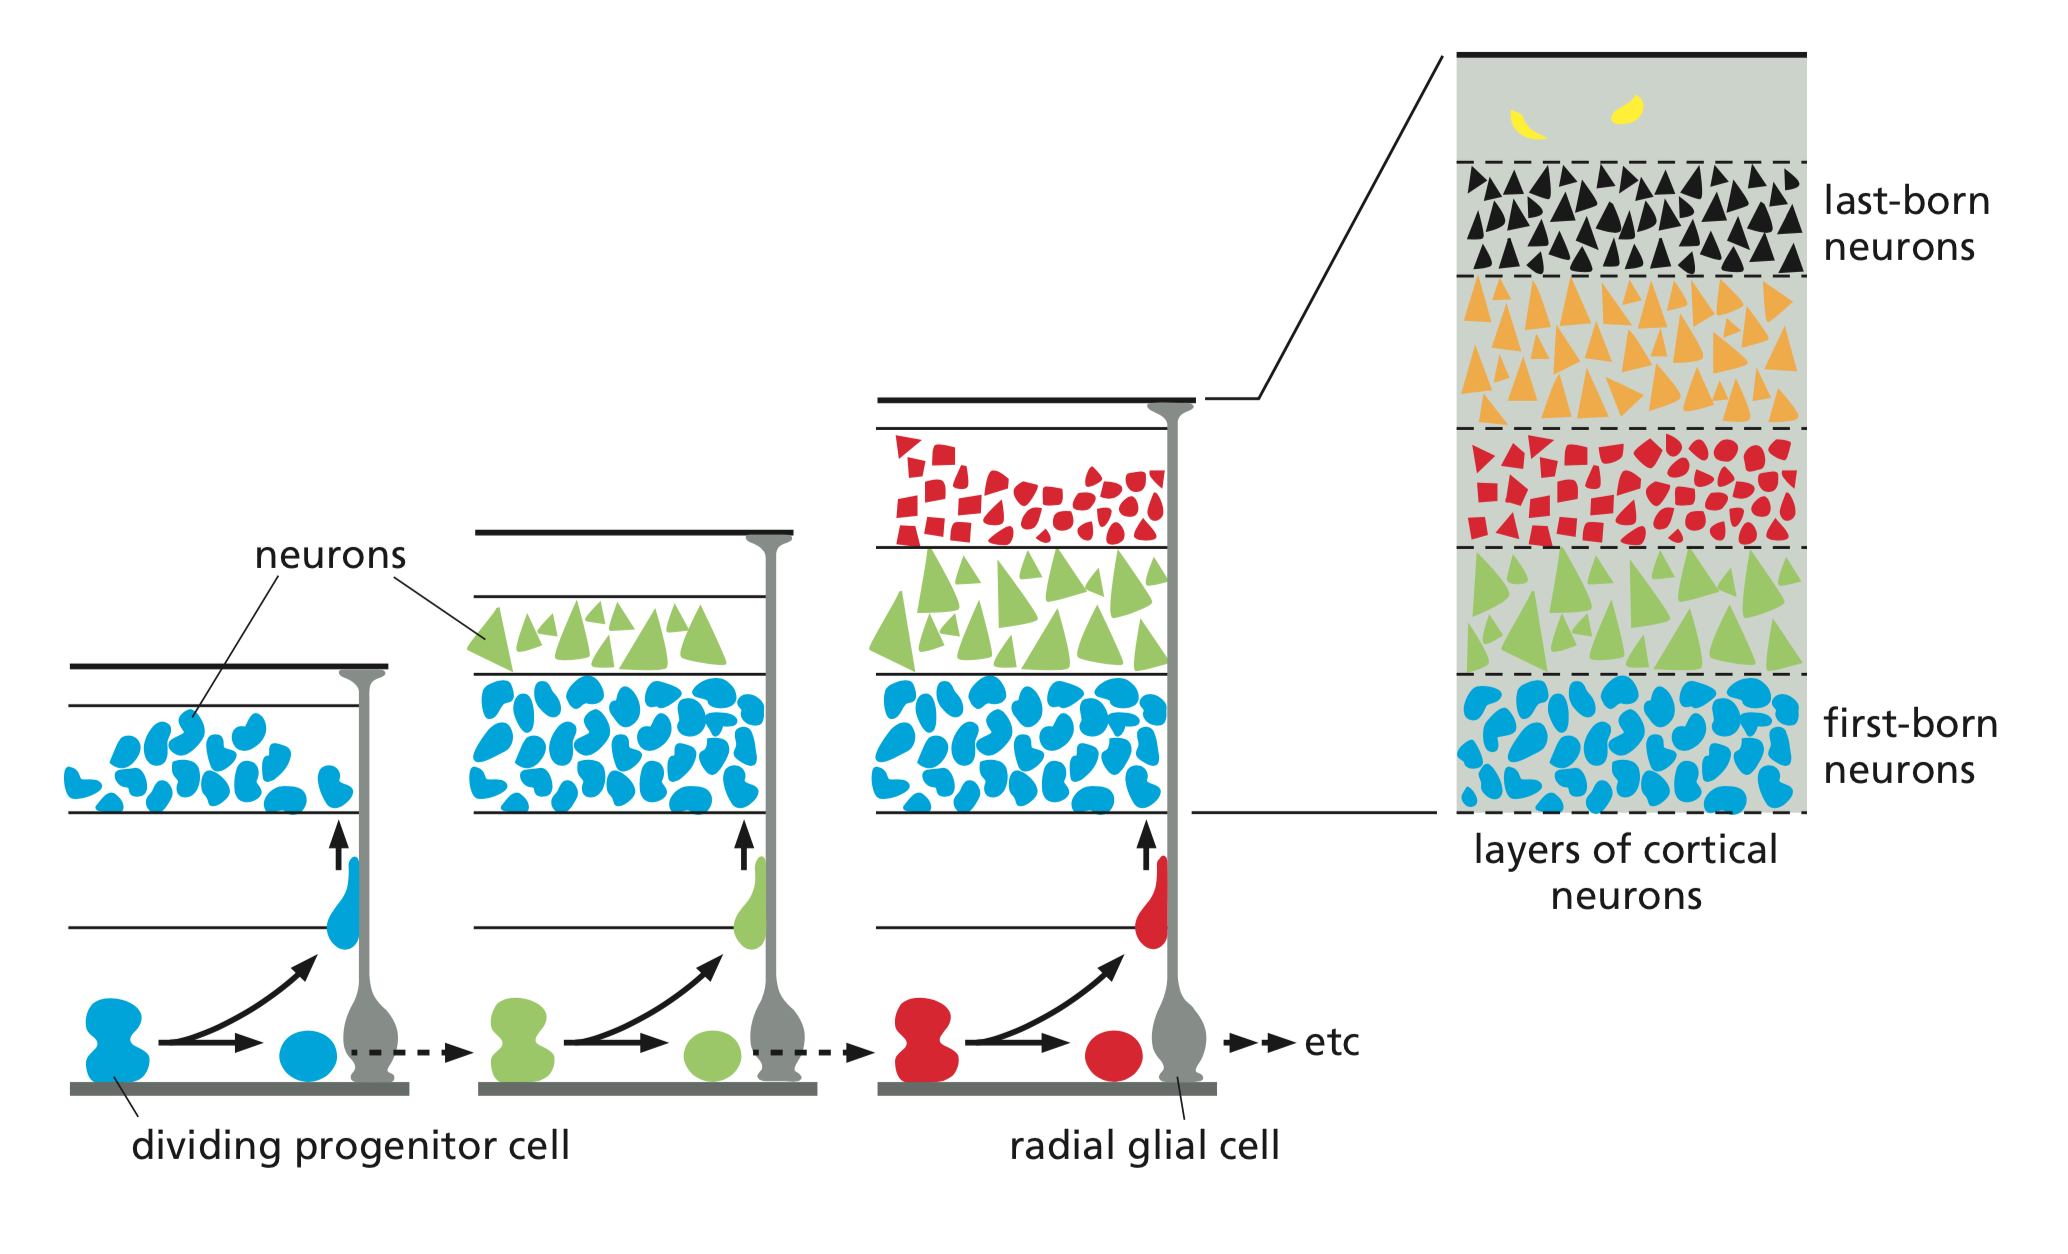
\includegraphics[width=0.85\textwidth]{vrstvy_rust.png}
    \centering
    \label{}
\end{figure}


\paragraph{Nervové spoje}
\begin{myItemize}[nosep]
    \item různé neurální populace se aktivují při různých úkolech
\begin{myItemize}[nosep]
    \item např. při rozlišování hranatých a kulatých věcí
\end{myItemize}

    \item dynamická struktura, která se "drátuje" v průběhu života
    \item součástí správného rozvoje CNS je i apoptóza
\begin{myItemize}[nosep]
    \item neurony, které nejsou za prvních pár týdnů prenatálního života použity, podléhají buněčné smrti
\end{myItemize}

    \item podobně jsou i v rámci postnatálního života posilovány spoje, které jsou často používány, naopak nepoužívané spoje slábnou a zanikají
\begin{myItemize}[nosep]
    \item je důležité dávat dítěti (alespoň do sedmi let života) co nejvíce různých vjemů
    \item příkladem může být absolutní hudební sluch, který silně souvisí s typem vjemů, kterým je dítě vystavováno
\begin{myItemize}[nosep]
    \item v Asii desetkrát vyšší incidence absolutního sluchu než u nás, snad kvůli tonálním jazykům
    \item je s ním spojený jen jeden gen, který však způsobuje i nízkou hodnotu IQ (čili tímto genem běžný absolutní sluch způsoben není)
\end{myItemize}

\end{myItemize}

    \item tato plasticita mozku během života zaniká
\begin{myItemize}[nosep]
    \item netvoří se nové spoje, pouze se posilují a zeslabují ty stávající
\end{myItemize}

\end{myItemize}



Místům v mozku, která byla původně určena jako nefunkční či prázdná, bývá pomocí FMR přiřazena funkce --- objevujeme stále nové souvislosti mezi jednotlivými částmi mozku.

\mybox{Poznámka}{\begin{description}
\item[mikrochimérismus]\hfill \\
Přítomnost dvou a více geneticky odlišných populací buněk, které jsou odvozeny z různých zdrojů, v jednom orgánu nebo jednotlivci.

Např. buňky myšátek během gravidity osidlují tělo matky, což se dá pozorovat na myšátkách GFP-tagovaného samce a netagované samice.

\end{description}
}


\subsection{Neurony} \label{Neurony}


\begin{myItemize}[nosep]
    \item schopné sčítat a odčítat signály z jiných neuronů, integrovat je, a pak vyslat signál
    \item jsou v podstatě zodpovědné za to, že myslíme
    \item neurony jdou připravit z kmenových buněk pomocí kyseliny retinové
\begin{myItemize}[nosep]
    \item na vytváření jednotlivých neurálních populací jsou potřeba ještědalší růstové faktory
\end{myItemize}

\end{myItemize}



\paragraph{Dendrity}
\begin{myItemize}[nosep]
    \item většina neuronů má mnoho dendritů
    \item větví se: co dendrit, to možnost napojit se na individuální nervovou buňku
\begin{myItemize}[nosep]
    \item např. Purkyněho buňky mohou integrovat až 200 000 signálů
\end{myItemize}

    \item při větvení se tenčí
    \item zesilují se, nebo zeslabují, podle toho, jak jsou používány
\begin{myItemize}[nosep]
    \item buňka umí do dendritu transportovat proteiny, snad tam umí i lokalizovat část translačního procesu
    \item tento proces nejspíše stojí za dlouhodobou pamětí
\end{myItemize}

\end{myItemize}



\paragraph{Axony}
\begin{myItemize}[nosep]
    \item většina neuronů má jeden axon, vzácně nula
    \item větví se, má ale konstantní šířku
    \item \si{1mm} -- \si{1m} na délku
    \item vyrůstají z místa zvaného \emph{axonální kónus}
\begin{myItemize}[nosep]
    \item tam se provádějí všechny výpočty
    \item jde o to, jestli je překročen akční potenciál
\end{myItemize}

    \item plazmatická membrána axolemma, obsahuje axoplazmu
    \item úsek mezi kónem a počátkem myelinové pochvy se nazývá \emph{iniciální segment}
\begin{myItemize}[nosep]
    \item jsou zde unikátní iontové kanály kontrolující generování nervového vzruchu
\end{myItemize}

    \item mohou být myelinizované i nemyelinizované
\end{myItemize}



\paragraph{Molecular fence}
\begin{myItemize}[nosep]
    \item zajišťuje diferenciaci na úrovni membrány
\begin{myItemize}[nosep]
    \item v axionálním výběžku jsou jiné iontové kanály než na dendritech
\end{myItemize}

    \item buňka je díky ní polarizovaná
    \item brání průchodu signalizace zpět do dendritu
    \item pro správnou funkci NS je nezbytná dostředivá a odstředivá signalizace právě na základě membránových domén
\end{myItemize}



\subsubsection{Nervová zakončení} \label{Nervová zakončení}


\begin{description}
\item[aktivační zakončení]\hfill \\
Extracelulárně snižují polaritu nebo koncentraci sodných iontů a zvyšují potenciální vybuzení neuronu k vypálení signálu. Způsobují malou depolarizaci na postsynaptické membráně, otevírají gated kationtové kanály.

Ve spojení především s neurotransmitery acetylcholinem a glutamátem.


\item[inhibiční zakončení]\hfill \\
Znesnadňují signalizaci buňkám, které se zrovna vylijí. Způsobují malou hyperpolarizaci, otevírají postsynaptické \(\ce{Cl-}\) a \(\ce{K+}\) kanály. Ovlivňují prostorovou a časovou sumaci signálů. Rozhodují o tom, jestli bude či nebude na neuronu postsynaptický potenciál.

Ve spojení především s neurotransmitery GABA a glycinem.

\end{description}


V reálu záleží na tom, jak se posčítají hyperpolarizace a depolarizace.

\paragraph{Funkce svalů}
\begin{myItemize}[nosep]
    \item motorický neuron musí dostat dostatečné množství aktivačních signálů
    \item sval samotný už nic neřeší a pokud dostane signál, prostě se stáhne
    \item akční potenciál je pořád stejně velký, jak rychle se má sval stáhnout pozná z frekvence, ve které dostává signály
\end{myItemize}



\subsubsection{Schopnost regenerace} \label{Schopnost regenerace}


\meta{Na toto byl v přednášce kladen velký důraz.}

Naproti všeobecné představě jsou nervové buňky schopny určité regenerace.

\mybox{Poznámka}{Nisslova substance (Nissl body) je granulární hmota v somě neuronu složená z endoplazmatického retikula obklopeného volnými ribozomy.}


\paragraph{Průběh poškození axonu}
\begin{myEnumerate}[nosep]
    \item Ve zdravém neuronu spojeném se svalem je jádro uprostřed a je v něm mnoho Nisslových substancí.
    \item Když je axon přerušen, jádro se posune na periferii a počet Nisslových substancí se sníží. Část nervového vlákna, která je nyní spojená jen se svalem, degeneruje a je odklizena makrofágy.
    \item Denervovaná svalová buňka atrofuje. Schwannovy buňky proliferují, tvoří silný kabel roustoucí ze svalové buňky.
    \item Axon dorůstá a snaží se spojit a prorůst Schwannovými buňkami.
\begin{myItemize}[nosep]
    \item Když se mu to povede, sval je opět inervovaný, obnoví se jeho síla i funkce a neuron se vrátí do původního stavu.
    \item Když se mu to nepovede, růst axonu je neorganizovaný, sval dál atrofuje. Po překročení určité doby je sval už nenávratně poškozen.
\end{myItemize}

\end{myEnumerate}



Axony málokdy najdou přesně tu správnou myelinovou pochvu a přesně to správné místo, kam původně vedly---jednotlivé svaly mají po regeneraci po zranění nejprve špatnou koordinaci a mozek se musí přeučovat, což trvá měsíce až roky.

U myši jsou schopna se zahojit i poranění páteře; při poraněních páteře u člověka je problém s tím, že je informační zmatek přerušených axonů obrovský, navíc axony by musely prorůst mnohem dál než u myši.

\paragraph{Léčba přerušených nervových spojů}
\begin{myItemize}[nosep]
    \item k léčení se snažíme využít i kmenové buňky
    \item stárnutí je spojeno s neurodegenerací, vymírají konkrétní populace nervových buněk
\begin{myItemize}[nosep]
    \item např. u Parkinsonovy choroby to jsou dopaminergní neurony v \emph{substantia nigra}
\end{myItemize}

    \item existují snahy diferencovat určité populace nervových buněk in vitro
    \item regenerace je ale omezenejší než u běžných epitelů
\begin{myItemize}[nosep]
    \item nejsilnější je regenerace v bulbus olfactorius (čichovém bulbu) a v hippokampu, který je plastický i v dospělosti
\end{myItemize}

\end{myItemize}



\paragraph{Příklady regenerace}
\begin{myItemize}[nosep]
    \item lze ji pozorovat u pacientů trpícími vážnými, život ohrožujícími epileptickými záchvaty
\begin{myItemize}[nosep]
    \item odstraní se velká část mozku s epileptickým ložiskem
    \item původní práci této části zastane druhá hemisféra
\end{myItemize}

    \item Phineas Gage
\begin{myItemize}[nosep]
    \item hlavou mu proletěla tyč
    \item obnovila se mu skvěle řeč i hybnost
\end{myItemize}

    \item víme, kde v myším mozku sídlí kmenové buňky
\end{myItemize}



\subsection{Pomocné nervové buňky} \label{Pomocné nervové buňky}


Mají základ z neurální trubice, v PNS z neurální lišty. Někdy jsou označované jako \textbf{gliové buňky}.

\begin{description}
\item[oligodendrocyty]\hfill \\
Tvoří myelinové pochvy axonů v CNS. Mohou se podílet na myelinizaci více než jednoho axonu.

Podobnou úlohu zastávají v PNS Schwannovy buňky. Každá Schwannova buňka však může vytvářet pouze jeden segment myelinové pochvy na jenom axonu.


\item[astrocyty]\hfill \\
Dělají strukturní a funkční podporu neuronům, ustanovují extracelulární homeostázi \(\ce{K+}\) a \(\ce{H+}\).

\paragraph{Funkce}
\begin{myItemize}[nosep]
    \item odstiňují synapse
    \item pomáhají vzruch vést, ale i ho zastavit
    \item dlouhé výběžky astrocytů slouží nervovým buňkám při jejich migraci do cílové struktury jako vodící struktury
    \item snižují hladinu draslíku a zvyšují hladinu sodíku v synapsi
    \item čistí extracelulární prostředí v mozku po proběhlých nervových vzruších
\end{myItemize}



Za jejich přítomnosti také dochází k vychytávání neurotransmiterů a k jejich transformaci; např. glutamát -> glutamin, který není neurotransmiterem. Glutamin poté předají presynaptickému neuronu. To se děje proto, aby k nervovým vzruchům mohlo docházet častěji.

\paragraph{Stavba}
\begin{myItemize}[nosep]
    \item diferenciace podléhá růstovým faktorům
\begin{myItemize}[nosep]
    \item NGF (nerve growth factor), BDGF (brain derived GF), GDNF (glial cell-derived neurotrophic factor)
\end{myItemize}

    \item navzájem propojeny gap junctions
    \item různé výběžky plní různé úkoly
\begin{myItemize}[nosep]
    \item nějaké výběžky obalují kapiláry a tvoří část hematoencefalytické bariéry
\end{myItemize}

\end{myItemize}




\item[mikroglie]\hfill \\
Imunokompetentní, mají podobnou funkci jako markofágy.


\item[ependymové buňky]\hfill \\
Pokrývají vnitřní dutiny CNS (trubice v míše a mozkové komory). Mají epiteloidní uspořádání a řasinky (povrch je velmi podobný epitelu dýchací trubic).

Jsou všude tam, kde je v CNS tekutina, kterou uvádějí v cirkulaci svými řasinkami.

\end{description}


\begin{figure}
    \caption{Schematický obrázek oligodendrocytu}
    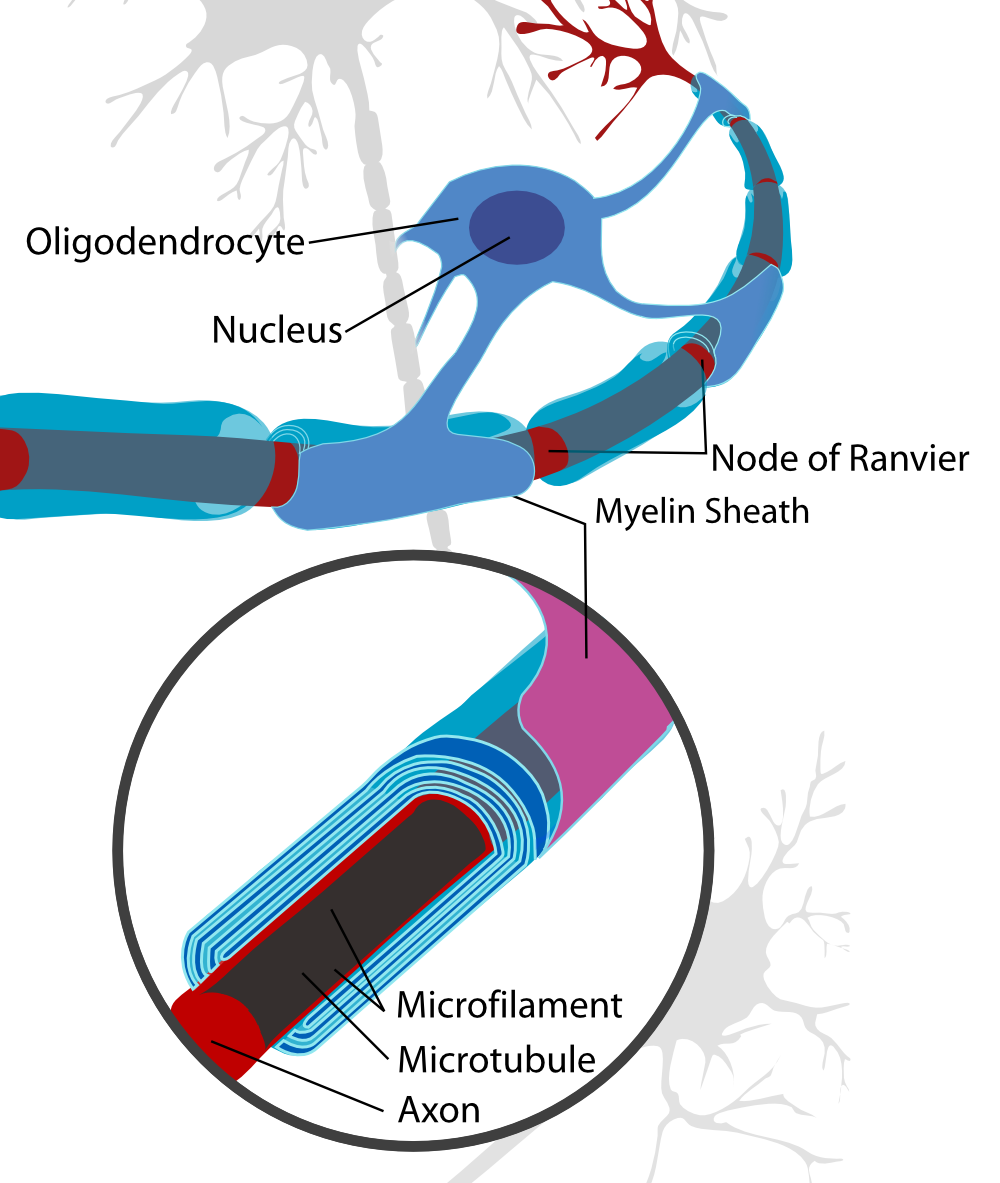
\includegraphics[width=0.85\textwidth]{oligodendrocyt.png}
    \centering
    \label{}
\end{figure}

\emph{By Neuron-with-oligodendrocyte-and-myelin-sheath.svg: *Complete-neuron-cell-diagram-en.svg: LadyofHatsderivative work: Andrew c (talk) - Neuron-with-oligodendrocyte-and-myelin-sheath.svg, Public Domain, \href{https://commons.wikimedia.org/w/index.php?curid=10888009}{link}}


Pro gliové buňky je základním zdrojem energie glukóza, kterou anaerobně štěpí na laktát. Kyslík je šetřen pro neurony, kde je potřeba pro přenos nervových vzruchů.

\paragraph{Myelinizace}
\begin{myItemize}[nosep]
    \item panožka Schwannovy buňky nebo oligodendrocytu se několikrát obtočí kolem výběžku
    \item výsledná vtsva má výborné elektrické vlastnosti
    \item nabohaceny komplexní glykolipidy, sfingolipidy, gangliosidy
    \item mnoho axonů není myelinizovaných, musí ale být odstíněné
\begin{myItemize}[nosep]
    \item invaginace na periferii, vchlípení do těla oligodendrocytu; vzniká \emph{mezaxon}
    \item v jednom kanálku může být i více axonů
\end{myItemize}

\end{myItemize}



\subsection{Hematoencefalická bariéra} \label{Hematoencefalická bariéra}


\begin{myItemize}[nosep]
    \item odděluje mozek od zbytku těla a je běžně pro buňky neprůchodná
    \item propouští kmenové buňky, pokud je v mozku indukováno poškození; minimálně u myší, na kterých byl tento experiment proveden
\begin{myItemize}[nosep]
    \item pronikají přes ni kmenové buňky neznámého původu
\begin{myItemize}[nosep]
    \item diferenciace v nervové buňky i různé typy gliových buněk
    \item zajištění regenerace poměrně velké části nervové tkáně
\end{myItemize}

\end{myItemize}

\end{myItemize}



Na obrázku lze pozorovat výběžky astrocytů, které k sobě těsně doléhají. Samotná kapilára je pak z endoteliálních buněk, které jsou spojeny přes tight junctions.

\begin{figure}
    \caption{Schematický obrázek hematoencefalické bariéry}
    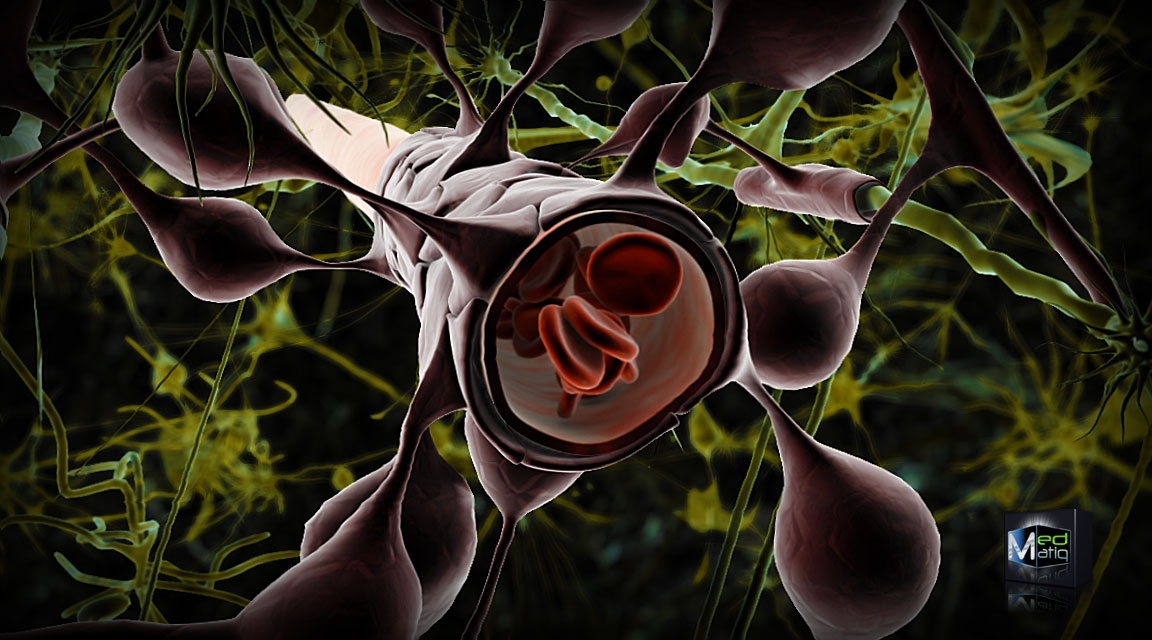
\includegraphics[width=0.85\textwidth]{bbb.jpg}
    \centering
    \label{}
\end{figure}

\emph{By Ben Brahim Mohammed - Own work, CC BY 3.0, \href{https://commons.wikimedia.org/w/index.php?curid=12263975}{link}}

\paragraph{Stavba}
\begin{myItemize}[nosep]
    \item endoteliání kapilární buňka je obklopena výběžky astrocytů
    \item všechny mezery mezi endoteliáními buňkami uzavřeny přes tight junctions
    \item kromě imunitních buněk by nemělo nic projít
    \item téměř vše, co se dostane k neuronům, prochází přes astrocyty
\end{myItemize}



\section{Senzorické epitely} \label{Senzorické epitely} \FloatBarrier


\begin{myItemize}[nosep]
    \item buňky na pomezí epitelu a nervové buňky
\begin{myItemize}[nosep]
    \item historicky je od ektodermu odvozena celá nervová soustava i senzorické tkáně čichové, zrakové i sluchové
\end{myItemize}

    \item mají apikální (detekční) a bazální (synaptický) konec
\end{myItemize}



\subsection{Čichový epitel} \label{Čichový epitel}


\begin{figure}
    \caption{Schéma čichového epitelu}
    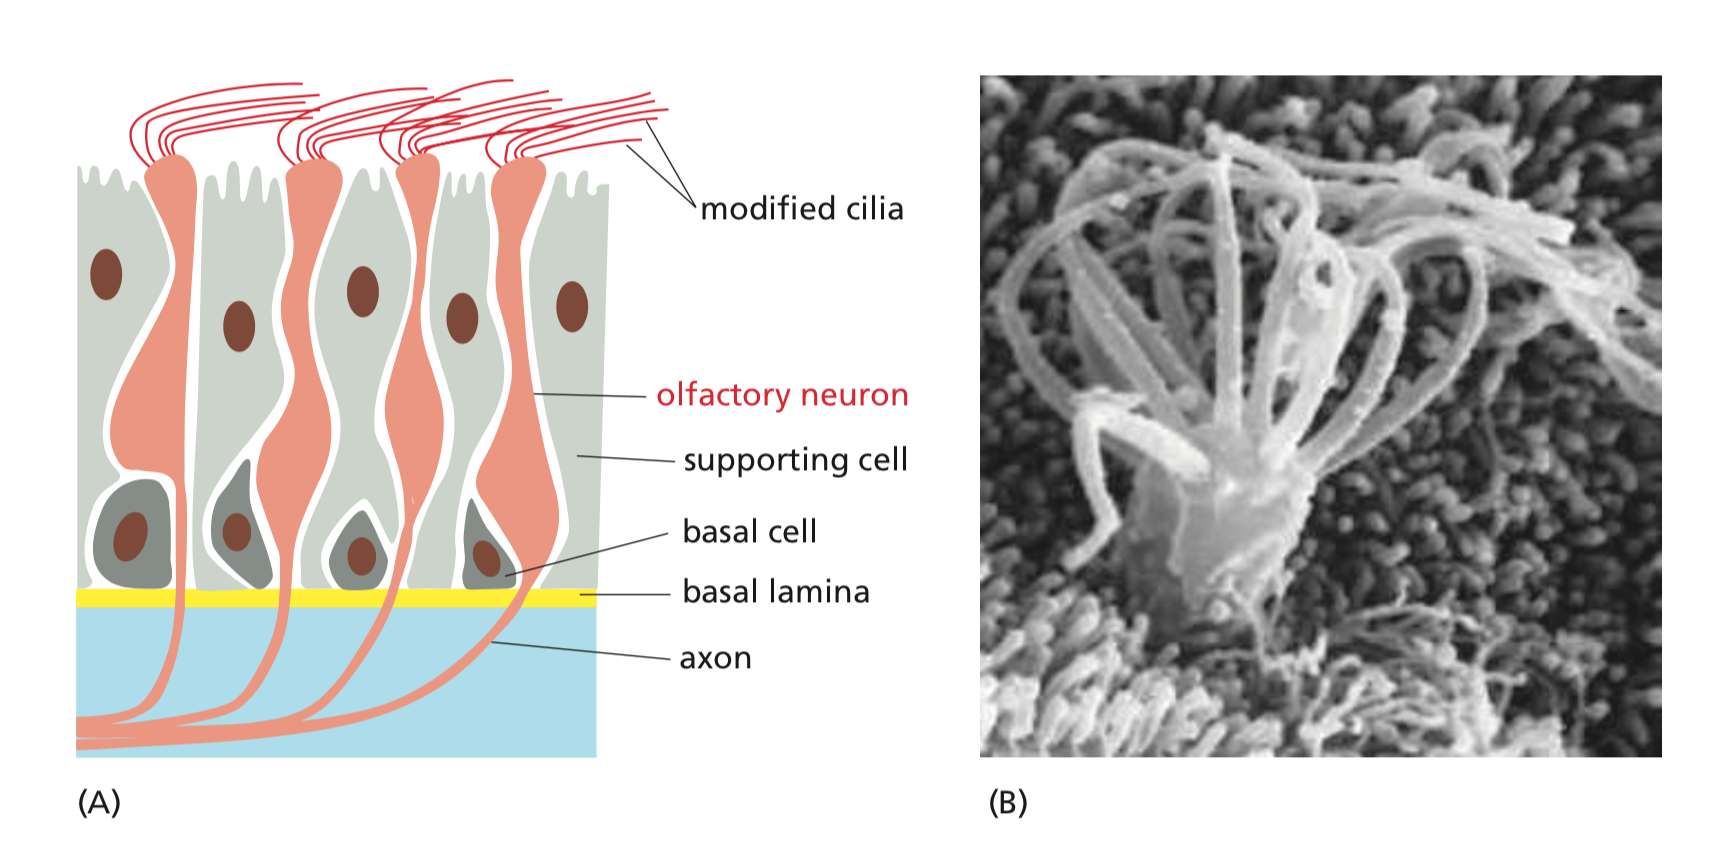
\includegraphics[width=0.85\textwidth]{nos.png}
    \centering
    \label{}
\end{figure}


\begin{myItemize}[nosep]
    \item jako jedna z mála neurosenzorických struktur se během života mění
\begin{myItemize}[nosep]
    \item senzorické neurony přežívají 1--2 měsíce
    \item poté jsou nahrazeny diferenciací bazálních buněk
\end{myItemize}

    \item skupina buněk se diferencuje v čichové (viz obrázek výše)
\begin{myItemize}[nosep]
    \item cilie jsou nepohyblivé, obsahují čichové receptory
    \item na bazální straně jeden axon směřující do mozku
    \item obklopeny podpůrnými buňkami s podobným významem jako gliové buňky
\end{myItemize}

    \item každý senzorický neuron exprimuje jen jeden z několika set čichových receptorů
\begin{myItemize}[nosep]
    \item když jsou buňky obnovovány, nově vznikající buňka si náhodně vybere jeden receptor
\end{myItemize}

\end{myItemize}



\paragraph{Glomeru­ly}
\begin{myItemize}[nosep]
    \item axony senzorických neuronů se stejným receptorem jsou rozptýleny v čichové sliznici (=> nejsou nashromážděny na jednom místě)
    \item axony neuronů se stejným receptorem směřují do stejného glomerulu
\begin{myItemize}[nosep]
    \item u myší je v bulbus olfactorius na každé straně 1800 různých glomerulů
    \item čím více glomerulů, tím více vůní umíme rozeznat, ale tím více druhů senzorických neuronů musíme mít
\end{myItemize}

    \item jak axony nově vznikajících buněk najdou správnou cestu ke glomerulu
\begin{myItemize}[nosep]
    \item zdá se, že v tom hrají roli receptory pro čich spřažené s G-proteiny
    \item tyto receptory jsou schopny homeotické adheze, tj. dva stejné receptory se "zazipují", ale dva různé ne
    \item axon putuje po glomerulech, zkouší se navázat a zůstane tam, kde se váže nejsilněji
\end{myItemize}

    \item existuje mnoho poruch této axonové navigace, lidé ztrácí schopnost kontinuity pachů
\end{myItemize}



Studium navigace axonů se opět provádělo na zelených myškách; zeleně se obarvily jen neurony reagující na jednu konkrétní vůni. Po histologii mozku se ukázalo, že všechny zelené axony míří pouze do dvou míst na bul­bus ol­fac­to­rius (dvou glomerulů, jednom v každé hemisféře).

\subsection{Sluchový epitel} \label{Sluchový epitel}


\begin{myItemize}[nosep]
    \item morfologicky nejpropracovanější tkáň v těle
    \item hlemýžďová rezonanční struktura vzniká prenatálně
    \item záleží na tom, v kterém místě hlemýždě dochází k rezonanci s membránami, které obalují prostory vyplněné tekutinou
\begin{myItemize}[nosep]
    \item u ústí hlemýždě jsou rozpoznávány vysoké frekvence, uprostřed spirály naopak nízké
    \item voda je nestlačitelná => přenáší vibrace
\end{myItemize}

    \item senzorickými buňkami jsou sluchové vláskové buňky
\end{myItemize}



\paragraph{Vláskové buňky}
\begin{myItemize}[nosep]
    \item leží ve struktuře \textbf{Cortiho orgánu} v hlemýždi, mezi podpůrnými buňkami, překryty extracelulární matrix
    \item převádějí mechanickou deformaci v elektrický signál
    \item všechny mají stejnou morfologii varhanovitých výběžků, \emph{stereocilií}
\begin{myItemize}[nosep]
    \item stabilizovány aktinovým cytoskeletem
    \item podobně jako výběžky na buňkách ve střevě
    \item rozměry každé stereocilie pevně dány vzhledem k poloze ve středním uchu, odpovídají frekvencii zvukového podnětu, na který mají reagovat
\end{myItemize}

    \item neregenerují se
    \item jsou propojené přes gap junctions \emph{konexinem 26}
\end{myItemize}



\begin{figure}
    \caption{Schematický obrázek popisující části vnitřního ucha}
    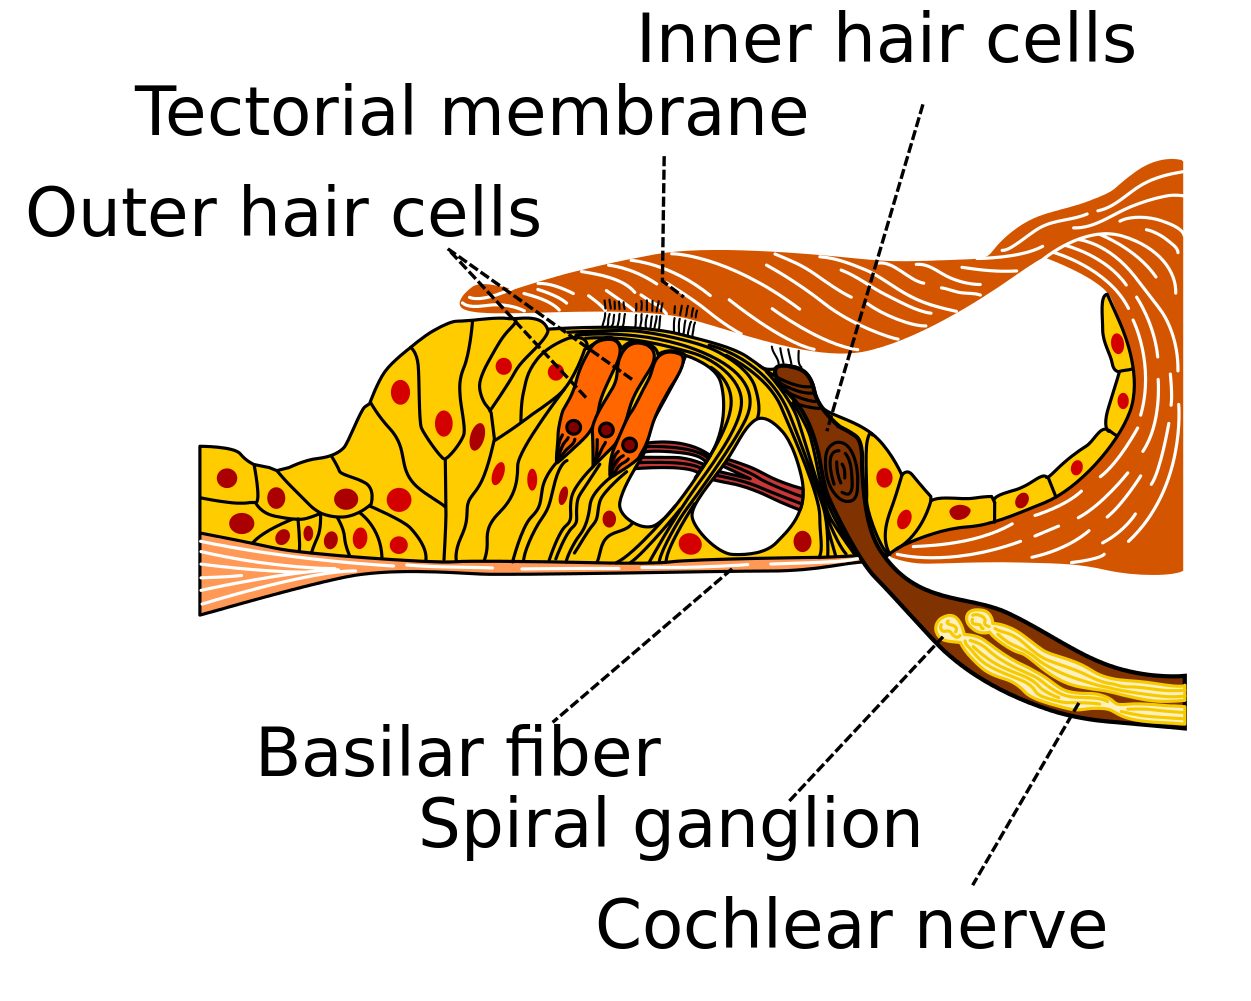
\includegraphics[width=0.85\textwidth]{ucho.png}
    \centering
    \label{}
\end{figure}

\emph{By Madhero88 - Own work, CC BY-SA 3.0, \href{https://commons.wikimedia.org/w/index.php?curid=6888273}{link}}

\paragraph{Princip funkce}
\begin{myEnumerate}[nosep]
    \item zvukové vibrace deformují stereocilia na vláskových buňkách
    \item otevírají se iontové kanály s mechanickými "vrátky" (mechanically gated ion channels)
\begin{myItemize}[nosep]
    \item reálně dochází ke změně konformace iontového kanálu
\end{myItemize}

    \item vzniká membránový vzruch, který se šíří vláskovou buňkou
    \item na bazálním konci dojde v synapsi s neuronem k vylití neurotransmiteru
\end{myEnumerate}



\paragraph{Choroby}
\begin{myItemize}[nosep]
    \item sluch se mění, hlavně ve stáří a hlavně mužům (špatný sluch zvláště ve vyšších frekvencích)
    \item celá řada poruch je genetického původu
\begin{myItemize}[nosep]
    \item mutace v konexinu 26 způsobují hluchotu (jedna z nejčastějších genetických chorob v Evropě)
\end{myItemize}

\end{myItemize}



\subsection{Zrakový epitel} \label{Zrakový epitel}


\begin{myItemize}[nosep]
    \item fotoreceptory se dělí na tyčinky a čípky
    \item senzorickou složkou jsou proteiny opsiny (\emph{ópsis} = zrak) s prostetickou skupinou \textbf{retinalem}
\begin{myItemize}[nosep]
    \item retinal je schopný cis-trans izomerizace, když pohltí foton
    \item změna konformace retinalu změní tvar opsinu
\end{myItemize}

    \item není schopný regenerace
\end{myItemize}



\begin{figure}
    \caption{Schéma vstevtanosti oka}
    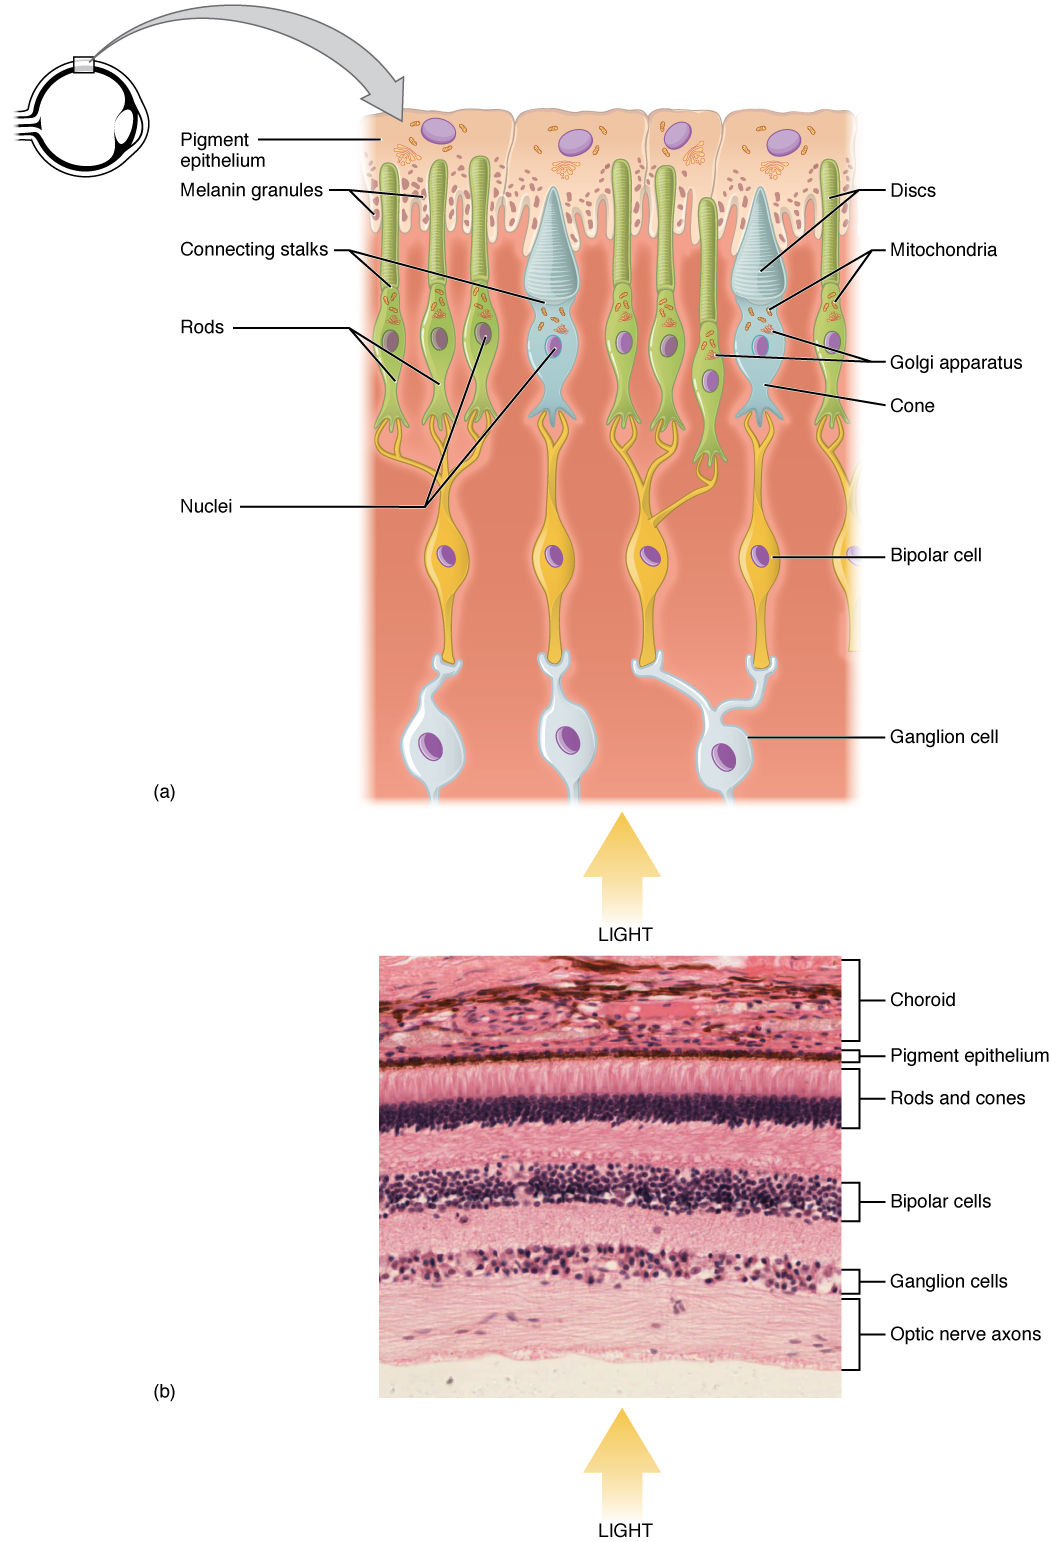
\includegraphics[width=0.85\textwidth]{oko.jpg}
    \centering
    \label{}
\end{figure}

\emph{[By OpenStax College - Anatomy Physiology, Connexions Web site. \href{http://cnx.org/content/col11496/1.6/}{author link}, Jun 19, 2013., CC BY 3.0, \href{https://commons.wikimedia.org/w/index.php?curid=30148002}{wiki link}]}

Nejblíže u pigmentovaných epiteliálních buněk je senzorický epitel, poté jsou různé interneurony a gangliové neurony, které vysílají signál do mozku. Apikální vrstvu senzorické složy tvoří brva (či přetvořený bičík).

\paragraph{Princip funkce v rámci buňky}
\begin{myEnumerate}[nosep]
    \item retinal změní konformaci
    \item opsin změní tvar
    \item aktivují se cGMP fosfodiesterázy, které štěpí cGMP
\begin{myItemize}[nosep]
    \item v očních buňkách je jinak vysoká koncentrace cGMP
\end{myItemize}

    \item otevřou se \(\ce{Ca^{2+}}\) kanály, dojde k hyperpolarizaci membrány
    \item uzavřou se \(\ce{Na+}\) kanály
    \item do synapse se přestane vylučovat neurotransmitter
    \item zastaví se bazální signalizace
\end{myEnumerate}



To, jakým způsobem vidíme, je vlastně negativ: při zachycení fotonu se sníží/zastaví bazální signalizace. To umožňuje rozlišovat jemnější nuance v signálech.

\paragraph{Tyčinky}
\begin{myItemize}[nosep]
    \item obsahují pigment rodopsin, který je součástí rodiny opsinů
    \item zajišťují vnímání kontrastu černé a bílé
\end{myItemize}


\paragraph{Čípky}
\begin{myItemize}[nosep]
    \item obsahují pigment jodopsin (fotopsin)
    \item zajišťují vnímání barev
    \item každý obsahuje jeden ze tří druhů jodopsinu (citlivý na červenou, zelenou, nebo modrou barvu)
\begin{myItemize}[nosep]
    \item vlastní barva vzniká superpozicí tří čípků
    \item mutace v jednom jodopsinu zapříčiní to, že člověk od sebe nebude schopen rozeznat určité barvy
\begin{myItemize}[nosep]
    \item např. daltonismus; jeden z jodopsinů je vázaný na chromozom X, takže se daltonismus vyskytuje častěji u mužů
\end{myItemize}

\end{myItemize}

\end{myItemize}




\paragraph{Pigmentované epiteliální buňky}
\begin{myItemize}[nosep]
    \item odrážejí a pohlcují světlo, brání odleskům
    \item fungují jako makrofágy
\begin{myItemize}[nosep]
    \item senzorické buňky se nemohou během života měnit, proto jen vyměňují svůj obsah
    \item odštěpují váčky s denaturovanými proteiny a kovalentně modifikovanými lipidy
    \item tyto váčky uklízejí právě epiteliální buňky
\end{myItemize}

\end{myItemize}



\paragraph{Choroby}
\begin{myItemize}[nosep]
    \item výše zmíněná barvoslepost
    \item mutace mitochondriální DNA => ztráta zraku, atrofie očního nervu
\begin{myItemize}[nosep]
    \item např. syndrom LHON
\begin{myItemize}[nosep]
    \item degenerace gangliových buněk
\end{myItemize}

    \item zrakový nerv a funkce senzorického zrakového epitelu je zřejmě jedna z Achillových pat energetického metabolismu
\end{myItemize}

\end{myItemize}



\section{Patologie nervové soustavy} \label{Patologie nervové soustavy} \FloatBarrier


\paragraph{Roztroušená skleróza}
\begin{myItemize}[nosep]
    \item autoimunitní onemocnění proti MBP (myelin basic protein)
    \item destrukce myelinových obalů T-lymfocyty
    \item nemoc můžeme experimentálně vyvolat u myši
\begin{myItemize}[nosep]
    \item např. tím, že přeneseme aktivované T-lymfocyty do těla
\end{myItemize}

    \item léčba je nákladná
\end{myItemize}



\paragraph{Epilepsie}
\begin{myItemize}[nosep]
    \item nervová soustava dočasně upadá do stavu pozitivních zpětných vazeb
    \item způsobená různými úrazy, infekcemi, někdy je dědičná
    \item jednou z příčin je odumření neuronů a nahrazení gliovými buňkami (tzv. \emph{gliová jizva})
\end{myItemize}



\paragraph{Parkinsonova choroba}
\begin{myItemize}[nosep]
    \item dochází ke svalovým třesům
    \item příčinou je nedostatek dopaminu
    \item v mozku jsou oblasti, kde jsou lokalizovány dopaminergní neurony (substantia nigra), ty často odumírají
    \item po Alzheimerovi druhá nejčastější choroba
\end{myItemize}



\paragraph{Alzheimerova choroba}
\begin{myItemize}[nosep]
    \item některé proteiny mají narušené odbourávání
\begin{myItemize}[nosep]
    \item např. amyloidní protein, \(\tau\) protein
\end{myItemize}

    \item v mozku se hromadí plaky neodbouratelné substance, která tlačí, je cytotoxická a způsobuje neurologické patologie
\end{myItemize}



\paragraph{Creutzfeld-Jacobova choroba}
\begin{myItemize}[nosep]
    \item prionové onemocnění
    \item chyby paměti, změny chování, špatná koordinace, časem slepota, slabost
    \item dost vzácná
    \item často se objeví zdánlivě bez příčiny, někdy je ale dědičná, dá se chytit i v rámci kontaktu s nakaženým nervovým systémem (např. při operacích)
    \item mozek po nakažení začne vypadat jako houba (s děrami)
\end{myItemize}



\paragraph{Nádory CNS}
\begin{myItemize}[nosep]
    \item primární nádory mozku tvoří přibližně 1--2\% všech zhoubných nádorů
    \item nejčastěji děti do pěti let, nebo dospělí od 60 let
    \item malé množství nádorů je dědičně podmíněno
    \item více než 50\% nádorů jsou nádory z buněk podpůrné tkáně, \emph{gliomy}
\begin{myItemize}[nosep]
    \item dělí se na low-grade a high-grade gliomy, podle toho, jak vysoký mají stupeň malignity
\end{myItemize}

    \item neuroblastom, ganglioneurom, feochromocytom, chemodektom, retinoblastom, oligodendrogliom (druh gliových buněk), astrocytom (druh gliových buněk), meduloblastom, ependymom, meningiom, angioretikulom
\end{myItemize}



\paragraph{Nádory PNS}
\begin{myItemize}[nosep]
    \item neurinom, neurilemom, neu­rofi­brom, Schwannom (nádor ze Schwannových buněk)
    \item neurogenní sarkom --- vzácná varianta neurinomu, maligní
\end{myItemize}


\end{document}